%----------------------------------------------------------
% EcoMesh -- Mini Project Report (SPIT, Computer Engineering, AY 2026-27)
%
% Page set-up follows the department's Mini Project / ESE report template
% (synopsis.tex): 12 pt, A4, single-sided, margins 20 mm left, right and top
% and 50 mm bottom, plain page style, 25-40 pages of report.  Preliminary
% pages follow Section 2 of the "Mini Project Report Preparation Guidelines"
% and the chapters follow its Section 3 (Chapters 1-11).
%
% Preliminary pages are numbered in roman numerals and the chapters from 1,
% so the 25-40 page count applies to the report itself.
%
% Build:  pdflatex main.tex  (run twice for the contents and lists)
%         or: tectonic -X compile main.tex --outdir build
% Overleaf: upload this whole folder, set main.tex as the main document.
%----------------------------------------------------------
\documentclass[12pt,a4paper,oneside]{article}
\usepackage[utf8]{inputenc}
\usepackage[T1]{fontenc}
\usepackage{lmodern}
\usepackage{epsfig}
\usepackage{graphicx}
\usepackage{cite}
\usepackage{geometry}
\usepackage{booktabs}
\usepackage{longtable}
\usepackage{array}
\usepackage{tabularx}
\usepackage{float}
\usepackage{placeins}
\usepackage{flafter}
\usepackage{needspace}
\usepackage{caption}
\usepackage{listings}
\usepackage{xcolor}
\usepackage{enumitem}
\usepackage{amsmath}
\usepackage{titlesec}
\usepackage{tocloft}
\usepackage{hyperref}

% ---- page set-up exactly as in the department template ----
\geometry{left=20mm,right=20mm,top=20mm,bottom=50mm}
\pagestyle{plain}

% ---- headings: each chapter starts on a new page with a "Chapter n" line ----
\setcounter{secnumdepth}{3}
\setcounter{tocdepth}{1}
\titleformat{\section}[display]
  {\normalfont\bfseries\centering}
  {\large CHAPTER \thesection}{6pt}{\LARGE}
  [\vspace{4pt}\titlerule]
\titleformat{name=\section,numberless}[block]
  {\normalfont\LARGE\bfseries\centering}{}{0pt}{}
\titlespacing*{\section}{0pt}{0pt}{12pt}
\titleformat{\subsection}{\normalfont\large\bfseries}{\thesubsection}{0.8em}{}
\titlespacing*{\subsection}{0pt}{10pt plus 2pt minus 2pt}{4pt plus 1pt}
\titleformat{\subsubsection}{\normalfont\normalsize\bfseries}{\thesubsubsection}{0.8em}{}
\titlespacing*{\subsubsection}{0pt}{8pt plus 2pt minus 2pt}{3pt}
\newcommand{\chapterpage}{\clearpage}
\let\oldsection\section
\renewcommand{\section}{\chapterpage\oldsection}
% a figure or table never appears before the text that introduces it (flafter)

% ---- contents, list of figures, list of tables ----
\renewcommand{\cfttoctitlefont}{\hfill\LARGE\bfseries}
\renewcommand{\cftaftertoctitle}{\hfill\mbox{}}
\renewcommand{\cftloftitlefont}{\hfill\LARGE\bfseries}
\renewcommand{\cftafterloftitle}{\hfill}
\renewcommand{\cftlottitlefont}{\hfill\LARGE\bfseries}
\renewcommand{\cftafterlottitle}{\hfill}
\renewcommand{\contentsname}{Table of Contents}
\setlength{\cftbeforetoctitleskip}{0pt}
\setlength{\cftbeforeloftitleskip}{0pt}
\setlength{\cftbeforelottitleskip}{14pt}
\setlength{\cftaftertoctitleskip}{16pt}
\setlength{\cftafterloftitleskip}{16pt}
\setlength{\cftafterlottitleskip}{16pt}
\renewcommand{\cftsecfont}{\bfseries}
\renewcommand{\cftsecpagefont}{\bfseries}
\renewcommand{\cftsecleader}{\bfseries\cftdotfill{\cftdotsep}}
\setlength{\cftbeforesecskip}{7pt}
\renewcommand{\cftsubsecfont}{\small}
\renewcommand{\cftsubsecpagefont}{\small}
\setlength{\cftsubsecindent}{1.6em}
\setlength{\cftsubsecnumwidth}{2.8em}
\renewcommand{\cftfigfont}{\footnotesize}
\renewcommand{\cftfigpagefont}{\footnotesize}
\renewcommand{\cfttabfont}{\footnotesize}
\renewcommand{\cfttabpagefont}{\footnotesize}
\renewcommand{\cftfigpresnum}{Figure }
\renewcommand{\cfttabpresnum}{Table }
\setlength{\cftfignumwidth}{5.2em}
\setlength{\cfttabnumwidth}{5.2em}
\setlength{\cftfigindent}{0pt}
\setlength{\cfttabindent}{0pt}
\setlength{\cftbeforefigskip}{0pt}
\setlength{\cftbeforetabskip}{0pt}

% ---- figures and tables: table titles above, figure titles below (template) ----
\captionsetup{font=small,labelfont=bf,labelsep=colon,justification=centering}
\captionsetup[table]{position=top,skip=4pt}
\captionsetup[figure]{position=bottom,skip=6pt}
\renewcommand{\topfraction}{0.9}
\renewcommand{\bottomfraction}{0.8}
\renewcommand{\textfraction}{0.07}
\renewcommand{\floatpagefraction}{0.75}
\setcounter{topnumber}{3}
\setcounter{bottomnumber}{2}
\setcounter{totalnumber}{5}
\setlength{\textfloatsep}{8pt plus 2pt minus 3pt}
\setlength{\floatsep}{8pt plus 2pt minus 2pt}
\setlength{\intextsep}{8pt plus 2pt minus 2pt}
% pages holding only figures/tables start at the top instead of being centred
\makeatletter\setlength{\@fptop}{0pt}\setlength{\@fpbot}{0pt plus 1fil}\makeatother
\renewcommand{\arraystretch}{1.05}
\newcolumntype{L}[1]{>{\raggedright\arraybackslash}p{#1}}

% ---- body text ----
\setlist{itemsep=2pt,topsep=4pt,parsep=0pt}
\setlength{\parskip}{0pt plus 1pt}
\emergencystretch=2em
\lstset{basicstyle=\ttfamily\footnotesize,breaklines=true,frame=single,columns=fullflexible,
        keepspaces=true,xleftmargin=2pt,xrightmargin=2pt,showstringspaces=false,aboveskip=6pt,belowskip=4pt}

\hypersetup{colorlinks=true,linkcolor=black,citecolor=black,urlcolor=black,
            pdftitle={EcoMesh: A Distributed Peer-to-Peer Disaster Relief Communication Mesh},
            pdfauthor={Miti Shah, Twissha Shah, Tanvi Sheth},
            pdfsubject={T.E. Computer Engineering Mini Project Report, SPIT, AY 2026-27},
            bookmarksnumbered=true}

\begin{document}
% Single place for names, UIDs and guide details used on the cover,
% certificates and declaration. UID pairing confirmed by the team.
\newcommand{\ProjectTitle}{EcoMesh: A Distributed Peer-to-Peer Disaster Relief Communication Mesh}
\newcommand{\ProjectTitleLineA}{EcoMesh: A Distributed Peer-to-Peer}
\newcommand{\ProjectTitleLineB}{Disaster Relief Communication Mesh}
\newcommand{\ProjectTitleShort}{EcoMesh}
\newcommand{\GroupNo}{Group 20}
\newcommand{\AcademicYear}{2026--27}
\newcommand{\Semester}{T.E. Semester V}
\newcommand{\CourseName}{Mini Project -- I}

\newcommand{\StudentA}{Miti Shah}
\newcommand{\UIDA}{2024300230}
\newcommand{\StudentB}{Twissha Shah}
\newcommand{\UIDB}{2024300231}
\newcommand{\StudentC}{Tanvi Sheth}
\newcommand{\UIDC}{2024300239}

\newcommand{\GuideName}{Prof. Anuj Tawari}
\newcommand{\HoDName}{Dr. Sudhir Dhage}
\newcommand{\PrincipalName}{Dr. B. N. Chaudhari}
\newcommand{\RepoURL}{https://github.com/tanvisheth1234-wq/miniproject}


% ================= preliminary pages (roman numerals) =================
\pagenumbering{roman}
\begin{titlepage}
\vspace*{0.025cm}
{\centering
{\Large\textbf {\ProjectTitle}}\\
\vspace{0.55cm}
Mini Project Report\\
submitted in partial fulfillment of the requirement\\
for the award of the Degree of\\\vspace{0.65cm}
{\large\textbf {Bachelor of Technology}}\\
in \\
{\large\textbf {Computer Engineering}}\\
\vspace{0.50cm}
by\\
\vspace{0.55cm}
{\large \textbf {\StudentA\ (UID \UIDA)}}\\
{\large \textbf {\StudentB\ (UID \UIDB)}}\\
{\large \textbf {\StudentC\ (UID \UIDC)}}\\
\vspace{0.3cm}
\GroupNo\ \textbullet\ \Semester\ \textbullet\ \CourseName\\
\vspace{0.55cm}
under the guidance of\\
\vspace{0.55cm}
\hspace{.05cm} {\large \textbf {\GuideName}}\\
\begin{figure}[h]
\centering

\includegraphics[scale=0.7]{spitlogo.pdf}
\end{figure}
\hspace{.05cm}
\hspace{.05cm}
\textbf{Department of Computer Engineering}\\
Bharatiya  Vidya Bhavan's\\
Sardar Patel Institute of Technology\\
(Autonomous Institute Affiliated to University of Mumbai)\\
Munshi Nagar, Andheri-West, Mumbai-400058\\
\vspace{0.4cm}
Academic Year \AcademicYear}
\end{titlepage}

\setcounter{page}{2}% the cover counts as page i
% Approval certificate: wording of the department Mini Project template
% (be_certificate2.tex); the signature blocks are a table so both columns align.
\clearpage
\thispagestyle{empty}
\vspace*{10mm}
\begin{center}
{\LARGE\bfseries Approval Certificate\par}
\end{center}
\vspace{12mm}
\noindent This is to certify that the Mini Project entitled \textbf{``\ProjectTitle''} by
\textbf{\StudentA}, \textbf{\StudentB} and \textbf{\StudentC} is approved for the partial fulfillment
of \CourseName\ for the Third Year Mini Project towards obtaining the Degree of Bachelor of Technology
in Computer Engineering.
\vspace{24mm}

\newcommand{\signblock}[1]{%
  \begin{minipage}[t]{70mm}
  \textbf{#1}\\[16mm]
  \rule{60mm}{0.4pt}\\
  (Signature)\\[6mm]
  Name: \rule{48mm}{0.4pt}\\[6mm]
  Date: \rule{49mm}{0.4pt}
  \end{minipage}}
\noindent\signblock{Project Guide}\hfill\signblock{External Examiner}

\vspace{24mm}
\noindent
\begin{tabular*}{\textwidth}{@{}l@{\extracolsep{\fill}}r@{}}
\rule{60mm}{0.4pt} & \rule{60mm}{0.4pt}\\
\textbf{Head of Department} & \textbf{Principal}\\
\end{tabular*}
\vfill
\begin{center}
\textbf{Seal of the Institute}
\end{center}
\vspace*{20mm}

% Declaration: wording of the department template (synopsis.tex), in the plural
% for a group, with names, UIDs and signatures in one aligned table.
\clearpage
\section*{Declaration}
\vspace{10mm}
\noindent We wish to state that the work embodied in this report titled ``\ProjectTitle'' forms our own
contribution to the work carried out under the guidance of \GuideName\ at the Sardar Patel Institute of
Technology. We declare that this written submission represents our ideas in our own words and where
others' ideas or words have been included, we have adequately cited and referenced the original sources.
We also declare that we have adhered to all principles of academic honesty and integrity and have not
misrepresented or fabricated or falsified any idea/data/fact/source in our submission. The report
distinguishes the features that are implemented and tested from those that are proposed, and every
reported result is supported by stored evidence.

\vspace{28mm}
\noindent
\begin{tabular*}{\textwidth}{@{}c@{\extracolsep{\fill}}c@{\extracolsep{\fill}}c@{}}
\rule{45mm}{0.4pt} & \rule{45mm}{0.4pt} & \rule{45mm}{0.4pt}\\
\textbf{\StudentA} & \textbf{\StudentB} & \textbf{\StudentC}\\
UID \UIDA & UID \UIDB & UID \UIDC\\
\end{tabular*}

\vspace{22mm}
\noindent
\begin{tabular}{@{}l@{\hspace{3mm}}l@{}}
\textbf{Date:} & \rule{50mm}{0.4pt}\\[8mm]
\textbf{Place:} & Mumbai\\
\end{tabular}


\clearpage
\section*{\centering{Acknowledgement}}
\vspace{1cm}
We would like to express our sincere gratitude to our project guide, \GuideName, for the direction, the regular reviews and the candid feedback that shaped this project from a problem statement into a working, measured system. His insistence that every claim be backed by evidence is reflected throughout this report.

We thank the Head of the Department of Computer Engineering and the Principal of the Sardar Patel Institute of Technology for providing the environment, the laboratory facilities and the opportunity to carry out this mini project. We are grateful to the faculty who coordinated the evaluation phases and the report guidelines, and to the examiners whose comments at the earlier phases improved the design.

Finally, we thank our classmates, who tested the demonstration and gave honest feedback on the interface, and our families for their support throughout the semester.

\vspace{1.5cm}
\begin{flushright}
\StudentA\\ \StudentB\\ \StudentC
\end{flushright}


\clearpage
\providecommand{\NTests}{334}\providecommand{\NRuns}{3}\providecommand{\NClean}{3}

\providecommand{\NFR}{68}\providecommand{\NAuto}{52}\providecommand{\NAutoUI}{10}\providecommand{\NPartial}{2}\providecommand{\NInspect}{2}\providecommand{\NManual}{2}

\providecommand{\CollN}{50}\providecommand{\CollDel}{92.6}\providecommand{\CollDelMin}{76}\providecommand{\CollDelMax}{100}\providecommand{\CollRecMean}{8.1}\providecommand{\CollRecMax}{10.25}\providecommand{\CollRecN}{50}\providecommand{\CollRecOK}{23}\providecommand{\CollConvMean}{9.6}\providecommand{\CollConvMax}{15.2}

\providecommand{\HopW}{99.2}\providecommand{\HopH}{57.4}\providecommand{\HopWins}{20}\providecommand{\HopRuns}{20}

\providecommand{\SosAdv}{4.4}

\providecommand{\NDevChecks}{21}\providecommand{\NDevPass}{21}\providecommand{\NWebChecks}{16}\providecommand{\NWebPass}{16}

\section*{Abstract}
\addcontentsline{toc}{section}{Abstract}

\textbf{Problem.} An earthquake, fire or collapse can take down the towers and internet links that every popular messaging application needs, although the phones of the people trapped inside can often still reach one another. Whatever connectivity survives helps only the person who holds it.

\textbf{Motivation and objectives.} Rescue is time-critical, so the aim is to let one person's connectivity serve everyone nearby and to let an SOS overtake routine traffic at every hop: a self-organising mesh, routing weighted by measured link quality, reliable delivery with a hold-and-forward fallback, encrypted and signed messages, and measured performance.

\textbf{Proposed solution.} In EcoMesh every device both sends and relays. A message moves device by device until it reaches a gateway with an outside link or a rescue device, or is held until a path appears. No internet, tower or server is needed.

\textbf{Technologies and engineering concepts.} Python \texttt{asyncio} (one event-loop thread per node); a 52-byte binary header of our own design; link-state gossip; Dijkstra over the cost $1+5(1-q)+3f$; a priority queue at every hop; ACK with retry and re-routing; AES-256-GCM and Ed25519; a SQLite log per node; FastAPI and WebSocket; React; and a transport interface that runs one engine on a simulator, on loopback and across laptops.

\textbf{Key implementation features.} Discovery with measured link quality; link-state flooding controlled by sequence numbers; duplicate suppression; a bounded hold queue that never drops an SOS for routine traffic; signatures that survive relaying; and one device app that becomes a survivor screen (hold-to-send SOS with nine request types, location, voice input, ``I am safe'', the rescue reply), a gateway view or a rescue console (requests with their route, replies, filters, history, CSV export, live map and activity panel).

\textbf{Testing methodology.} \NTests\ automated tests (unit, integration, boundary, fuzz, replay, concurrency, a three-node mesh over TCP), a test mapping for all 68 requirements, seven seeded simulator scenarios, loss and scale sweeps to 65 nodes, five live processes over real sockets, and scripted browser checks of the device screens (\NDevPass\ of \NDevChecks\ pass).

\textbf{Results.} A 40-node mesh at 20\,\% loss with injected failures delivered \CollDel\,\% of messages (50 runs). On identical seeds weighted routing delivered \HopW\,\% against \HopH\,\% for hop count. Under load an SOS had a \SosAdv$\times$ lower median latency than routine traffic. On five live processes an SOS arrived in a median 32\,ms, a sender re-routed around a failed relay in a median 4.1\,s, and every message held during a gateway outage was delivered. Convergence and recovery met their targets on average but not in every run; at 20\,\% loss delivery stayed above 90\,\% to 50 nodes and fell to 83.1\,\% at 65.

\textbf{Practical applicability and limitations.} EcoMesh can serve today as an institutional safety network on laptops. The radio is emulated by a LAN restricted to configured neighbours, so it is not yet phone to phone; a Bluetooth or Wi-Fi Direct transport, adaptive timers, a usability study and per-pair keys are the main future work.


\clearpage
\phantomsection\addcontentsline{toc}{section}{Table of Contents}
\tableofcontents
\clearpage
\phantomsection\addcontentsline{toc}{section}{List of Figures}
\listoffigures
\renewcommand{\chapterpage}{\vspace{2em}}
\phantomsection\addcontentsline{toc}{section}{List of Tables}
\listoftables
\renewcommand{\chapterpage}{\clearpage}
\clearpage
\section*{List of Abbreviations and Symbols}
\addcontentsline{toc}{section}{List of Abbreviations and Symbols}
\footnotesize
\renewcommand{\arraystretch}{1.0}
\begin{longtable}{L{3.2cm}L{12.4cm}}
\toprule
\textbf{Term} & \textbf{Meaning}\\ \midrule \endhead
ACK & Acknowledgement packet returned by the destination along the reverse path\\
AES-256-GCM & Advanced Encryption Standard, 256-bit key, Galois/Counter Mode (authenticated encryption)\\
AODV & Ad hoc On-Demand Distance Vector routing (RFC 3561)\\
API & Application Programming Interface\\
ASGI & Asynchronous Server Gateway Interface (used by FastAPI/uvicorn)\\
BLE & Bluetooth Low Energy\\
DAA & Design and Analysis of Algorithms\\
DBMS & Database Management System\\
DFD & Data Flow Diagram\\
DTN & Delay-Tolerant Networking (RFC 4838)\\
Ed25519 & Edwards-curve Digital Signature Algorithm over Curve25519\\
ER & Entity--Relationship (diagram)\\
ESE & End Semester Evaluation\\
FR / NFR & Functional / Non-Functional Requirement\\
GATEWAY & Node role: has a link to the outside world; valid terminal for \texttt{RESCUE\_\_}\\
HELLO & Periodic one-hop beacon used for neighbour discovery\\
KPI & Key Performance Indicator\\
LAN & Local Area Network\\
MANET & Mobile Ad hoc Network\\
OLSR & Optimized Link State Routing (RFC 3626)\\
OS & Operating System\\
PWA & Progressive Web App\\
RESCUE & Node role: rescue-team device; valid terminal for \texttt{RESCUE\_\_}\\
\texttt{RESCUE\_\_} & Symbolic destination meaning ``the nearest GATEWAY or RESCUE node''\\
SF / S\&F & Store-and-Forward\\
SOS & Highest message priority (value 0)\\
SRS & Software Requirements Specification\\
TCP / UDP & Transmission Control Protocol / User Datagram Protocol\\
TTL & Time To Live (remaining hop allowance of a packet)\\
UML & Unified Modeling Language\\
WAL & Write-Ahead Logging (SQLite journal mode)\\
$V$, $E$ & Number of vertices (nodes) and edges (links) of the mesh graph\\
$q$ & Link quality in $[0,1]$: fraction of the last 20 expected HELLOs received\\
$f$ & Recent failures: ACK timeouts attributed to a link in the last 60\,s\\
$C_{max}$, $T_{hold}$ & Store-and-forward bounds: maximum count (500) and maximum age (1800\,s)\\
\bottomrule
\end{longtable}


% ================= report (arabic numerals from Chapter 1) =================
\clearpage
\pagenumbering{arabic}
\setcounter{table}{0}
\setcounter{figure}{0}
\section{Introduction and Problem Definition}
\label{ch:intro}

\subsection{Project Background}
After an earthquake, fire or collapse the mobile network and internet link are usually the first to fail or saturate, yet connectivity survives in pockets (a person near a window with one bar of signal, an access point on a UPS, a rescue team's kit) that help only their owner. \textbf{EcoMesh} turns every participating device into both a sender and a relay, so a message can travel from device to device until it reaches its addressee, a \emph{gateway} that still has an outside link, or a \emph{rescue} device, without the internet and without a server.

\subsection{Problem Statement}
WhatsApp, Signal, Telegram and SMS all need a distant server or tower; when a Wi-Fi router loses its uplink they all stop, although the phones on it can still exchange packets. Trapped people then cannot report their condition, share the one weak signal, coordinate or be located quickly. Existing offline systems either flood messages or route by hop count, give no priority to emergencies, publish few measurements, and in one widely deployed case were shown to lack effective confidentiality and authenticity~\cite{albrecht2021bridgefy} (Chapter~\ref{ch:lit}).

\subsection{Motivation}
Survival depends on how soon rescuers learn who is inside, where, and in what condition. Sharing one person's connectivity with everyone nearby and pushing an SOS ahead of routine traffic at every hop shortens that delay for trapped occupants, rescue teams, and the hospitals, campuses, hostels, factories and stadiums that could install it in advance.

\subsection{Objectives}
O1 \emph{Self-organising mesh}: neighbours are found automatically and every node learns the whole graph within 15\,s. O2 \emph{Weighted routing} that outperforms hop count on identical scenarios. O3 \emph{Priority}: an SOS overtakes routine traffic at every hop, with a median latency at least 3$\times$ lower under load. O4 \emph{Reliability}: at least 90\,\% delivery on 40 nodes at 20\,\% loss, and a new route within 10\,s of a relay failure. O5 \emph{Store-and-forward}: a message without a route is kept, never dropped, and is delivered when a route returns. O6 \emph{Security}: payloads stay confidential and tamper-evident, and a forged SOS is rejected. O7 \emph{Evidence}: every metric is computed from the nodes' own logs. O8 \emph{Integration}: a web front end, a REST and WebSocket back end and the engine running together on several devices.

\subsection{Scope of the Project}
\textbf{Included:} discovery, a binary wire protocol, link-state gossip, Dijkstra routing over a link-quality cost, per-hop priority, TTL, duplicate suppression, acknowledgement with retry, heartbeats, node roles, bounded store-and-forward, AES-256-GCM and Ed25519, a SQLite log per node, \texttt{asyncio} concurrency, a simulator with metrics, and survivor and rescue screens. \textbf{Excluded:} a real Bluetooth LE or Wi-Fi Direct transport, NAT traversal, voice calls, video and file transfer, machine learning and a native mobile app. \textbf{Users:} the trapped person, the relay user, the gateway operator and the rescue coordinator. \textbf{Environment and scale:} laptops running Python~3.10 on a shared network, five live devices and up to 65 simulated nodes. One design decision is stated plainly: the mesh runs over LAN sockets that stand in for Bluetooth LE or Wi-Fi Direct, and each node may talk only to the neighbours listed for it, which imitates limited radio range. Discovery, routing, reliability and encryption sit above the transport, so a radio transport can replace the sockets without changing them.

\subsection{Proposed Solution}
Each device runs one node, a Python process whose \texttt{asyncio} loop handles discovery, gossip, receiving, sending, store-and-forward and a small web server. A message leaves by one of three exits: a \textbf{gateway} with an outside link (reaching any gateway counts as delivery); a \textbf{rescue} device that comes into range and receives every pending SOS; or \textbf{store-and-forward}, where a node with no route keeps the message, so a person walking out carries others' messages out. Paths are chosen by Dijkstra's algorithm on a graph whose edge weights penalise weak and failing links (Chapter~\ref{ch:alg}).

\subsection{Novelty and Originality}
EcoMesh combines \textbf{priority-aware, link-quality-weighted routing with a delay-tolerant fallback, and evaluates it by measurement}. SOS priority is applied again at every hop. The link cost is derived from measured HELLO reception and from acknowledgement failures, and a failure raises the cost immediately. A single transport interface lets the same engine run on a simulator, on loopback and on separate laptops. Every reported number is a query over the nodes' logs, and weighted and hop-count routing are compared on the same seeds.

\subsection{Feasibility Analysis}
\textbf{Technical:} all components are mature open-source software, and the largest risk, debugging routing over live sockets, was removed by building the simulator first. \textbf{Economic:} the system uses existing laptops and free software and needs no server, so there is no running cost. \textbf{Operational:} one command starts a node, and the survivor screen has one prominent control. \textbf{Time and resources:} three members over one semester, about 336 person-hours, delivered in four tagged phases.

\subsection{Social Relevance and Practical Applications}
The realistic path is \emph{installation before an incident}: an institution puts EcoMesh on staff and resident devices as part of its safety plan and rescue teams carry it as standard kit, so the rescue exit exists even if no civilian has it. Survivors are found faster at no infrastructure cost.

\subsection{Success Criteria and Key Performance Indicators}
\label{sec:kpi}
Table~\ref{tab:kpi} lists the quantified requirements of the SRS, fixed before testing began; Section~\ref{sec:kpival} checks each against measured data.
\begin{table}[!htbp]
\caption{Key performance indicators}
\label{tab:kpi}
\footnotesize
\begin{tabularx}{\textwidth}{@{}>{\raggedright\arraybackslash}p{3.6cm}>{\raggedright\arraybackslash}X>{\raggedright\arraybackslash}p{1.9cm}>{\raggedright\arraybackslash}p{3.5cm}@{}}
\toprule
\textbf{KPI} & \textbf{Definition} & \textbf{Target} & \textbf{Measured by}\\ \midrule
K1 Delivery & Delivered $\div$ sent, 40 nodes, 20\,\% loss & $\ge$ 90\,\% & seeded simulator runs\\
K2 Convergence & Every node's graph holds every node & $\le$ 15\,s & simulator, live\\
K3 Recovery & Relay death until a route avoiding it & $\le$ 10\,s & 50 trials, live\\
K4 SOS advantage & Median routine $\div$ median SOS latency under load & $\ge$ 3$\times$ & burst scenario\\
K5 Store-and-forward & Retained messages flushed on return & 100\,\% & simulator, live\\
K6 Weighted vs hop count & Delivery on identical seeds & weighted better & paired runs\\
K7 Scale & Nodes within the targets & $\ge$ 50 & sweep 10--65 nodes\\
K8 UI freshness & Event to screen & $\le$ 2\,s & API time, poll interval\\
K9 Correctness & Tests passed & 100\,\% & repeated runs\\
K10 Security & No relay decryption; forged SOS and tampering rejected & all hold & automated tests\\
\bottomrule
\end{tabularx}
\end{table}

\section{Literature Review and Study of Existing Systems}
\label{ch:lit}

\subsection{Study of Existing Systems}
\textbf{Offline messengers.} \emph{Bridgefy}, a Bluetooth messenger used at large protests, is Study~11 of Table~\ref{tab:studies}; \emph{FireChat} offered phone-to-phone chat and was withdrawn; \emph{Briar} needs no server and exchanges encrypted messages over Bluetooth or Wi-Fi when devices meet~\cite{briar}. \textbf{Dedicated radios.} \emph{goTenna Mesh} pairs phones with radio units; \emph{Meshtastic} uses LoRa with a controlled flood in which a node stays silent if a neighbour already repeats the packet~\cite{meshtastic}. \textbf{Research and humanitarian work.} The \emph{Serval Project} builds disaster phone meshes with its \emph{Rhizome} store-and-forward layer~\cite{serval}; the \emph{delay-tolerant networking (DTN)} architecture keeps data and carries it across intermittent links~\cite{fall2003dtn,rfc4838}. ``n/d'' marks a property the sources do not document.
\subsection{Review of Research Papers and Technical Resources}
\label{sec:papers}
Table~\ref{tab:studies} summarises the twelve sources we studied, what each contributes and what it means for EcoMesh.
\begingroup\footnotesize
\setlength{\tabcolsep}{3pt}
\begin{longtable}{@{}p{0.5cm}>{\raggedright\arraybackslash}p{3.5cm}p{6.3cm}p{6.0cm}@{}}
\caption{Twelve studies: technique, contribution and relevance to EcoMesh}\label{tab:studies}\\
\toprule \textbf{\#} & \textbf{Source} & \textbf{Technique and contribution} & \textbf{Relevance and limitation}\\ \midrule \endfirsthead
\toprule \textbf{\#} & \textbf{Source} & \textbf{Technique and contribution} & \textbf{Relevance and limitation}\\ \midrule \endhead
1 & DSDV, Perkins and Bhagwat 1994~\cite{perkins1994dsdv} & Each node keeps a table of distances in advance; numbered updates stop routing loops & Routes exist before the first SOS; counts hops only, and update traffic rises as nodes move\\
2 & DSR, RFC 4728~\cite{rfc4728dsr} & Routes are found on demand and the whole path is written into each packet & A carried path allows loop checks and the ``relayed via $n$'' display; nothing is held\\
3 & AODV, RFC 3561~\cite{rfc3561aodv} & A flooded request finds a destination and the reply sets up the route backwards & Counts hops; no holding of messages and no priority\\
4 & OLSR, RFC 3626~\cite{rfc3626olsr} & Link state maintained in advance; selected relays reduce repeated broadcasts & Nearest relative of EcoMesh; still uses hop count by default\\
5 & OSPF v2, RFC 2328~\cite{rfc2328ospf} & Numbered link-state flooding with Dijkstra run on each router & EcoMesh keeps this structure but uses a measured cost; designed for wired links\\
6 & Babel, RFC 8966~\cite{rfc8966babel} & Loop-free distance vector for wireless meshes with any metric plugged in & Shows the wireless metric must be replaceable; covers routing only\\
7 & ETX, De Couto et al. 2003~\cite{decouto2003etx} & Path cost from measured delivery ratios; shows that fewest-hop paths choose lossy links & Main basis for our cost; we add a penalty for acknowledgement failures\\
8 & Epidemic routing, Vahdat and Becker 2000~\cite{vahdat2000epidemic} & Copy every message to every node encountered & Delivers well but fills buffers; we use one bounded queue instead\\
9 & DTN architecture, Fall 2003; RFC 4838~\cite{fall2003dtn,rfc4838} & Nodes keep, carry and later pass on data, with custody handed over & Basis of our third exit; ignores priority and link quality\\
10 & Disaster-response networks, Reina et al. 2015~\cite{reina2015disaster} & Survey of ad hoc, vehicular, delay-tolerant and sensor networks in disasters & Supports our framing and the call for systems that are evaluated\\
11 & Breaking Bridgefy, Albrecht et al. 2021~\cite{albrecht2021bridgefy} & Attacks on a real mesh messenger: users tracked, messages unauthenticated, network shut down & Defines our threat model; motivates encryption and signatures\\
12 & AES-GCM, Ed25519, Dijkstra~\cite{nist80038d,bernstein2012ed25519,dijkstra1959} & Authenticated encryption, fast secure signatures and shortest paths & The primitives and routing algorithm we use\\
\bottomrule
\end{longtable}
\endgroup

\subsection{Comparative Analysis}
\label{sec:compare}
Table~\ref{tab:compare1} sets the systems of Section~2.1 and the protocols of Table~\ref{tab:studies} against EcoMesh: the infrastructure each needs, how it routes, whether it prioritises, whether it keeps a message that has no route, and how it protects content.
\begin{table}[!htbp]
\caption[Existing systems and routing protocols compared with EcoMesh]{Existing offline-communication systems and routing protocols compared with EcoMesh (n/d = not documented in the sources consulted)}
\label{tab:compare1}
\footnotesize
\begin{tabularx}{\textwidth}{@{}>{\raggedright\arraybackslash}p{2.1cm}>{\raggedright\arraybackslash}X>{\raggedright\arraybackslash}X>{\raggedright\arraybackslash}p{1.7cm}>{\raggedright\arraybackslash}p{1.9cm}>{\raggedright\arraybackslash}X@{}}
\toprule
\textbf{System} & \textbf{Infrastructure} & \textbf{Routing} & \textbf{Priority} & \textbf{Store-fwd} & \textbf{Encryption}\\ \midrule
Bridgefy & Bluetooth LE phones & n/d & n/d & n/d & none effective in analysed version~\cite{albrecht2021bridgefy}\\
Briar & none (Bluetooth/Wi-Fi, Tor) & direct device sync & n/d & on contact & end-to-end~\cite{briar}\\
Meshtastic & LoRa radios & managed flood~\cite{meshtastic} & n/d & n/d & channel-level\\
Serval & Wi-Fi ad hoc phones & B.A.T.M.A.N., later own & n/d & yes (Rhizome)~\cite{serval} & n/d\\
DTN & none & architecture only & bundle class of service & yes (custody) & separate specification\\
AODV, DSR, DSDV, OLSR, OSPF, Babel & none & hop count, configured or pluggable metric & none & none or short & not in protocol\\
\textbf{EcoMesh} & \textbf{none} & \textbf{link state, weighted Dijkstra} & \textbf{3 levels, every hop} & \textbf{yes, bounded} & \textbf{AES-GCM + Ed25519}\\
\bottomrule
\end{tabularx}
\end{table}

\subsection{Limitations of Existing Systems}
Hop count, the usual default metric, picks lossy links~\cite{decouto2003etx}; no system prioritises an emergency at each hop; ad hoc routing drops a message with no route, while delay-tolerant designs keep it but ignore link quality and priority; and deployed messengers publish little measurement, one with no effective confidentiality or authenticity~\cite{albrecht2021bridgefy}.
\subsection{Identified Research or Engineering Gap}
\label{sec:gap}
\textbf{None of the surveyed systems joins priority-aware, link-quality-weighted routing with a delay-tolerant fallback, and none is evaluated quantitatively under controlled failures.}
\subsection{Proposed Improvements}
EcoMesh routes over the cost $1+5(1-q)+3f$ (Section~\ref{sec:cost}), re-applies SOS priority at each hop, holds unroutable messages in a bounded queue that never evicts an SOS for routine traffic, uses vetted cryptography, and measures all of it, including weighted against hop-count routing.

\section{Software Requirements Specification}
\label{ch:srs}

\subsection{Purpose and Scope of the SRS}
This chapter condenses the IEEE 830 Software Requirements Specification delivered in Phase~II (\texttt{docs/SRS\_EcoMesh\_Group20.pdf}). It states \emph{what} EcoMesh must do, not how. The scope is a single deployment of cooperating nodes with ten system features (peer discovery, message composition, multi-hop forwarding, adaptive routing, priority handling, reliability, store-and-forward, message security, logging, rescue dashboard); no server exists in any operating mode.

\subsection{Intended Users and Stakeholders}
The \emph{trapped user} originates an SOS or a message and needs one prominent control and no configuration. The \emph{relay user} passively carries other people's traffic and must not be able to read it. The \emph{gateway operator} holds the residual outside link. The \emph{rescue coordinator} monitors the SOS queue, the topology and delivery statistics. The \emph{administrator} assigns node identifiers and constrains who hears whom. The project guide and evaluators review scope, rigour and evidence.

\subsection{Overall Product Description}
Every node runs the same program. HELLO beacons build a neighbour table; link-state reports build a graph; Dijkstra selects next hops; a per-hop priority queue orders transmissions; ACK, retry, deduplication and store-and-forward give reliability; AES-256-GCM and Ed25519 give confidentiality and authenticity; and an embedded web server exposes the node to a browser. The operating environment is an IP network segment on which infrastructure services have failed; where multicast is blocked a configured peer list is used (DIS-7). Dependencies are the Python runtime and the \texttt{cryptography} library.

\subsection{Functional Requirements}
\label{sec:fr}
The 68 functional requirements are listed in Table~\ref{tab:fr}. Each has a unique identifier, its text, and an acceptance criterion: the tests that must pass (and, for screens, a manual check). Each feature's input, processing and output are given in the feature's heading row.
\begingroup\footnotesize\renewcommand{\arraystretch}{1.0}
\setlength{\tabcolsep}{3pt}
\begin{longtable}{@{}p{1.25cm}p{6.3cm}p{1.65cm}p{6.95cm}@{}}
\caption[Functional requirements and their acceptance tests]{Functional requirements by feature (identifiers as in the SRS). Check: Auto = verified by automated tests, Auto+UI = automated tests plus a manual check of the screen, Partial = only partly implemented, Inspect = code inspection, Manual = manual check only; * marks a mapped test that failed once in repeated runs. The first mapped test is named and (+n) counts the others.}\\
\label{tab:fr}\\
\toprule \textbf{ID} & \textbf{Requirement (the system shall \ldots)} & \textbf{Check} & \textbf{Acceptance criterion: tests that must pass} \\ \midrule \endfirsthead
\toprule \textbf{ID} & \textbf{Requirement} & \textbf{Check} & \textbf{Acceptance criterion} \\ \midrule \endhead
\multicolumn{4}{@{}p{16.78cm}@{}}{\rule{0pt}{7pt}\textbf{3.4.1 Peer discovery.} \textit{Input:} HELLO beacons (role, public key) from neighbours; silence from a known neighbour. \textit{Processing:} Update the neighbour table; estimate link quality over a 20-HELLO window; prune after the timeout. \textit{Output:} Peer-up and peer-down events and link quality passed to routing.} \\ \midrule
DIS-1 & transmit a discovery beacon at a fixed, configurable interval. & Auto & \texttt{test\_\allowbreak{}hello\_\allowbreak{}is\_\allowbreak{}broadcast\_\allowbreak{}on\_\allowbreak{}start} \\
DIS-2 & keep a neighbour table with node id, address, role, public key, last-seen time and measured link quality. & Auto & \texttt{test\_\allowbreak{}update\_\allowbreak{}reports\_\allowbreak{}new\_\allowbreak{}neighbour\_\allowbreak{}once} (+3) \\
DIS-3 & add a previously unknown node to the table on receipt of a valid beacon. & Auto & \texttt{test\_\allowbreak{}neighbour\_\allowbreak{}added\_\allowbreak{}on\_\allowbreak{}hello\_\allowbreak{}received} (+1) \\
DIS-4 & declare a neighbour unreachable after a configurable period of silence. & Auto & \texttt{test\_\allowbreak{}neighbour\_\allowbreak{}marked\_\allowbreak{}dead\_\allowbreak{}after\_\allowbreak{}timeout} (+1) \\
DIS-5 & compute link quality as the proportion of expected beacons received over a sliding window. & Auto & \texttt{test\_\allowbreak{}perfect\_\allowbreak{}reception\_\allowbreak{}scores\_\allowbreak{}one} (+2) \\
DIS-6 & operate without manual configuration of peer addresses. & Auto & \texttt{test\_\allowbreak{}message\_\allowbreak{}to\_\allowbreak{}discovered\_\allowbreak{}neighbour\_\allowbreak{}delivers\_\allowbreak{}without\_\allowbreak{}manual\_\allowbreak{}next\_\allowbreak{}hop} (+1) \\
DIS-7 & support an optional configured seed list of peers where multicast is unavailable. & Auto & \texttt{test\_\allowbreak{}visible\_\allowbreak{}neighbours\_\allowbreak{}filters\_\allowbreak{}unlisted\_\allowbreak{}senders} (+1) \\
\multicolumn{4}{@{}p{16.78cm}@{}}{\rule{0pt}{7pt}\textbf{3.4.2 Message composition and transmission.} \textit{Input:} Text and destination, or the SOS control (sustained press). \textit{Processing:} Build a packet with a unique id and timestamp; encrypt and sign; queue. \textit{Output:} DATA packet sent; delivery state shown to the user.} \\ \midrule
MSG-1 & let a user compose and send a text message to a named node. & Auto+UI & \texttt{test\_\allowbreak{}send\_\allowbreak{}with\_\allowbreak{}ack\_\allowbreak{}delivers\_\allowbreak{}and\_\allowbreak{}gets\_\allowbreak{}acknowledged} (+3) \\
MSG-2 & let a user address a message to the rescue service rather than a specific node. & Auto & \texttt{test\_\allowbreak{}rescue\_\allowbreak{}dst\_\allowbreak{}routes\_\allowbreak{}to\_\allowbreak{}gateway\_\allowbreak{}across\_\allowbreak{}multiple\_\allowbreak{}hops} (+1) \\
MSG-3 & provide a distinct SOS control that requires a sustained press. & Auto+UI & \texttt{test\_\allowbreak{}sos\_\allowbreak{}reaches\_\allowbreak{}the\_\allowbreak{}rescue\_\allowbreak{}queue\_\allowbreak{}and\_\allowbreak{}the\_\allowbreak{}sender\_\allowbreak{}sees\_\allowbreak{}it\_\allowbreak{}delivered} \\
MSG-4 & assign a globally unique identifier to every message it originates. & Auto & \texttt{test\_\allowbreak{}msg\_\allowbreak{}id\_\allowbreak{}defaults\_\allowbreak{}to\_\allowbreak{}uuid4\_\allowbreak{}and\_\allowbreak{}round\_\allowbreak{}trips} (+1) \\
MSG-5 & record the creation time of every message it originates. & Auto & \texttt{test\_\allowbreak{}timestamp\_\allowbreak{}is\_\allowbreak{}uint64\_\allowbreak{}milliseconds} (+1) \\
MSG-6 & display the current delivery state of each originated message. & Auto+UI & \texttt{test\_\allowbreak{}store\_\allowbreak{}logs\_\allowbreak{}sent\_\allowbreak{}message\_\allowbreak{}and\_\allowbreak{}delivery\_\allowbreak{}lifecycle} (+1) \\
MSG-7 & display the number of intermediate nodes traversed by a delivered message. & Auto+UI & \texttt{test\_\allowbreak{}update\_\allowbreak{}message\_\allowbreak{}route\_\allowbreak{}records\_\allowbreak{}hops\_\allowbreak{}and\_\allowbreak{}path} (+1) \\
\multicolumn{4}{@{}p{16.78cm}@{}}{\rule{0pt}{7pt}\textbf{3.4.3 Multi-hop forwarding.} \textit{Input:} DATA or ACK packet from a neighbour. \textit{Processing:} Validate; drop duplicates; check hop allowance and loop; append own id; queue by priority. \textit{Output:} Packet forwarded, or dropped with a logged reason.} \\ \midrule
FWD-1 & forward packets not addressed to it towards the destination. & Auto & \texttt{test\_\allowbreak{}two\_\allowbreak{}hop\_\allowbreak{}relay\_\allowbreak{}a\_\allowbreak{}to\_\allowbreak{}b\_\allowbreak{}to\_\allowbreak{}c} (+1) \\
FWD-2 & decrement the remaining hop allowance of every packet it forwards. & Auto & \texttt{test\_\allowbreak{}on\_\allowbreak{}forward\_\allowbreak{}hook\_\allowbreak{}called\_\allowbreak{}with\_\allowbreak{}next\_\allowbreak{}hop} \\
FWD-3 & discard any packet whose hop allowance has reached zero. & Auto & \texttt{test\_\allowbreak{}drops\_\allowbreak{}when\_\allowbreak{}ttl\_\allowbreak{}expired} \\
FWD-4 & append its own identifier to the traversal path of every forwarded packet. & Auto & \texttt{test\_\allowbreak{}on\_\allowbreak{}forward\_\allowbreak{}hook\_\allowbreak{}called\_\allowbreak{}with\_\allowbreak{}next\_\allowbreak{}hop} (+1) \\
FWD-5 & discard any packet whose traversal path already contains its own identifier. & Auto & \texttt{test\_\allowbreak{}drops\_\allowbreak{}on\_\allowbreak{}loop\_\allowbreak{}detected} \\
FWD-6 & validate the structure of a packet before any forwarding decision. & Auto & \texttt{test\_\allowbreak{}bad\_\allowbreak{}magic\_\allowbreak{}rejected} (+3) \\
FWD-7 & be unable to read the payload of a packet it merely forwards. & Auto & \texttt{test\_\allowbreak{}relay\_\allowbreak{}never\_\allowbreak{}sees\_\allowbreak{}plaintext\_\allowbreak{}payload} \\
\multicolumn{4}{@{}p{16.78cm}@{}}{\rule{0pt}{7pt}\textbf{3.4.4 Adaptive routing.} \textit{Input:} Link-state reports; a destination. \textit{Processing:} Merge into the graph; Dijkstra over the weighted cost; resolve RESCUE\_\_ to the nearest gateway or rescue node. \textit{Output:} Least-cost next hop; routes recomputed on topology change.} \\ \midrule
RTE-1 & periodically transmit its own neighbour list to adjacent nodes. & Auto & \texttt{test\_\allowbreak{}send\_\allowbreak{}report\_\allowbreak{}reaches\_\allowbreak{}each\_\allowbreak{}neighbour} (+1) \\
RTE-2 & construct a graph of the network from received link-state reports. & Auto & \texttt{test\_\allowbreak{}receiving\_\allowbreak{}report\_\allowbreak{}merges\_\allowbreak{}reported\_\allowbreak{}edges\_\allowbreak{}into\_\allowbreak{}graph} (+1) \\
RTE-3 & compute least-cost paths using Dijkstra's algorithm over the weighted graph. & Auto & \texttt{test\_\allowbreak{}shortest\_\allowbreak{}path\_\allowbreak{}multi\_\allowbreak{}hop\_\allowbreak{}chain} (+1) \\
RTE-4 & derive link cost from a base hop penalty, measured link quality and recent delivery failures. & Auto & \texttt{test\_\allowbreak{}edge\_\allowbreak{}cost\_\allowbreak{}matches\_\allowbreak{}section\_\allowbreak{}8\_\allowbreak{}2\_\allowbreak{}formula} (+1) \\
RTE-5 & recompute routes whenever the topology changes. & Auto & \texttt{test\_\allowbreak{}record\_\allowbreak{}failure\_\allowbreak{}invalidates\_\allowbreak{}cached\_\allowbreak{}routes} (+2) \\
RTE-6 & treat any node advertising the gateway or rescue role as a valid terminal for rescue-service messages. & Auto & \texttt{test\_\allowbreak{}rescue\_\allowbreak{}dst\_\allowbreak{}resolves\_\allowbreak{}to\_\allowbreak{}nearest\_\allowbreak{}gateway} (+2) \\
RTE-7 & select the least-cost terminal when several are reachable. & Auto & \texttt{test\_\allowbreak{}rescue\_\allowbreak{}dst\_\allowbreak{}picks\_\allowbreak{}cheapest\_\allowbreak{}of\_\allowbreak{}multiple\_\allowbreak{}gateways} \\
RTE-8 & converge on a consistent topology view within a bounded interval after a change. & Auto & \texttt{test\_\allowbreak{}report\_\allowbreak{}reflooded\_\allowbreak{}reaches\_\allowbreak{}a\_\allowbreak{}node\_\allowbreak{}two\_\allowbreak{}hops\_\allowbreak{}away} (+1) \\
\multicolumn{4}{@{}p{16.78cm}@{}}{\rule{0pt}{7pt}\textbf{3.4.5 Priority handling.} \textit{Input:} Packets of different priority queued together. \textit{Processing:} Priority queue ordered by priority, then age, applied at every hop. \textit{Output:} SOS transmitted before routine traffic.} \\ \midrule
PRI-1 & support three priority levels: SOS, NORMAL, STATUS. & Auto & \texttt{test\_\allowbreak{}all\_\allowbreak{}three\_\allowbreak{}priorities\_\allowbreak{}ordered\_\allowbreak{}correctly} (+1) \\
PRI-2 & keep outgoing messages in a priority queue rather than a FIFO queue. & Auto & \texttt{test\_\allowbreak{}sos\_\allowbreak{}pops\_\allowbreak{}before\_\allowbreak{}normal\_\allowbreak{}regardless\_\allowbreak{}of\_\allowbreak{}insertion\_\allowbreak{}order} \\
PRI-3 & apply priority ordering at every hop, not only at the originator. & Auto & \texttt{test\_\allowbreak{}sos\_\allowbreak{}forwarded\_\allowbreak{}before\_\allowbreak{}already\_\allowbreak{}queued\_\allowbreak{}normal} (+1) \\
PRI-4 & order messages of equal priority by creation time, oldest first. & Auto & \texttt{test\_\allowbreak{}ties\_\allowbreak{}broken\_\allowbreak{}by\_\allowbreak{}oldest\_\allowbreak{}timestamp\_\allowbreak{}first} \\
PRI-5 & assign SOS priority to every message generated by the SOS control. & Auto+UI & \texttt{test\_\allowbreak{}sos\_\allowbreak{}reaches\_\allowbreak{}the\_\allowbreak{}rescue\_\allowbreak{}queue\_\allowbreak{}and\_\allowbreak{}the\_\allowbreak{}sender\_\allowbreak{}sees\_\allowbreak{}it\_\allowbreak{}delivered} \\
PRI-6 & display the priority level of each message in the interface. & Manual & \textit{Priority badges are shown on the screens (manual check); no automated UI test.} \\
\multicolumn{4}{@{}p{16.78cm}@{}}{\rule{0pt}{7pt}\textbf{3.4.6 Reliability.} \textit{Input:} Delivered or unacknowledged packets; duplicates; missing beacons. \textit{Processing:} ACK; timer; retry with a recomputed route; dedup set; failure detection. \textit{Output:} ACK returned; bounded retries; duplicates dropped; failed neighbours removed.} \\ \midrule
REL-1 & carry a hop allowance in every packet and decrement it at each hop. & Auto & \texttt{test\_\allowbreak{}drops\_\allowbreak{}when\_\allowbreak{}ttl\_\allowbreak{}expired} (+2) \\
REL-2 & remember recently observed message identifiers for a configurable period. & Auto & \texttt{test\_\allowbreak{}entry\_\allowbreak{}expires\_\allowbreak{}after\_\allowbreak{}window} (+1) \\
REL-3 & discard any packet whose identifier is already remembered. & Auto & \texttt{test\_\allowbreak{}duplicate\_\allowbreak{}delivery\_\allowbreak{}is\_\allowbreak{}dropped} (+2) \\
REL-4 & transmit an acknowledgement on successful delivery. & Auto & \texttt{test\_\allowbreak{}send\_\allowbreak{}with\_\allowbreak{}ack\_\allowbreak{}delivers\_\allowbreak{}and\_\allowbreak{}gets\_\allowbreak{}acknowledged} (+1) \\
REL-5 & retransmit an unacknowledged message after a configurable timeout. & Auto & \texttt{test\_\allowbreak{}timeout\_\allowbreak{}triggers\_\allowbreak{}retry\_\allowbreak{}and\_\allowbreak{}resets\_\allowbreak{}timer} (+1) \\
REL-6 & recompute the route before each retransmission. & Auto & \texttt{test\_\allowbreak{}record\_\allowbreak{}failure\_\allowbreak{}updates\_\allowbreak{}graph\_\allowbreak{}immediately\_\allowbreak{}not\_\allowbreak{}just\_\allowbreak{}on\_\allowbreak{}next\_\allowbreak{}report} (+1) \\
REL-7 & abandon delivery after a configurable number of failed attempts and mark the message accordingly. & Auto & \texttt{test\_\allowbreak{}exhausting\_\allowbreak{}max\_\allowbreak{}retries\_\allowbreak{}reports\_\allowbreak{}failed\_\allowbreak{}and\_\allowbreak{}stops\_\allowbreak{}tracking} (+1) \\
REL-8 & detect node failure through absence of discovery beacons and update the graph. & Auto & \texttt{test\_\allowbreak{}route\_\allowbreak{}forgotten\_\allowbreak{}when\_\allowbreak{}neighbour\_\allowbreak{}dies} (+2) \\
\multicolumn{4}{@{}p{16.78cm}@{}}{\rule{0pt}{7pt}\textbf{3.4.7 Store-and-forward.} \textit{Input:} A message with no route; a new route or neighbour. \textit{Processing:} Bounded retention by count and age; periodic flush; lowest priority evicted first. \textit{Output:} Message delivered when a path appears, or expired and logged.} \\ \midrule
SNF-1 & retain a message when route computation yields no path. & Auto & \texttt{test\_\allowbreak{}send\_\allowbreak{}without\_\allowbreak{}route\_\allowbreak{}queues\_\allowbreak{}to\_\allowbreak{}store\_\allowbreak{}forward} \\
SNF-2 & periodically re-attempt delivery of retained messages. & Auto & \texttt{test\_\allowbreak{}store\_\allowbreak{}forward\_\allowbreak{}flushes\_\allowbreak{}once\_\allowbreak{}a\_\allowbreak{}route\_\allowbreak{}appears} \\
SNF-3 & attempt delivery of retained messages immediately on detecting a new neighbour. & Auto & \texttt{test\_\allowbreak{}held\_\allowbreak{}message\_\allowbreak{}is\_\allowbreak{}sent\_\allowbreak{}the\_\allowbreak{}moment\_\allowbreak{}its\_\allowbreak{}neighbour\_\allowbreak{}appears} (+1) \\
SNF-4 & bound the retention queue by both message count and retention period. & Auto & \texttt{test\_\allowbreak{}enqueue\_\allowbreak{}over\_\allowbreak{}the\_\allowbreak{}bound\_\allowbreak{}evicts\_\allowbreak{}lowest\_\allowbreak{}priority} (+2) \\
SNF-5 & discard the lowest-priority retained messages first when the bound is reached. & Auto & \texttt{test\_\allowbreak{}enqueue\_\allowbreak{}over\_\allowbreak{}the\_\allowbreak{}bound\_\allowbreak{}evicts\_\allowbreak{}lowest\_\allowbreak{}priority} (+2) \\
SNF-6 & report the number of retained messages in the interface. & Manual & \textit{The held-message count is shown on the screens (manual check); no automated UI test.} \\
\multicolumn{4}{@{}p{16.78cm}@{}}{\rule{0pt}{7pt}\textbf{3.4.8 Message security.} \textit{Input:} Payload and packet identity fields. \textit{Processing:} AES-256-GCM encryption; Ed25519 signature; verification and decryption on receipt. \textit{Output:} Tampered or forged packets rejected.} \\ \midrule
SEC-1 & encrypt message payloads using authenticated symmetric encryption. & Auto & \texttt{test\_\allowbreak{}encrypt\_\allowbreak{}decrypt\_\allowbreak{}round\_\allowbreak{}trip} (+2) \\
SEC-2 & ensure intermediate nodes cannot recover the plaintext of messages they forward. & Auto & \texttt{test\_\allowbreak{}relay\_\allowbreak{}never\_\allowbreak{}sees\_\allowbreak{}plaintext\_\allowbreak{}payload} \\
SEC-3 & sign the packet header and traversal path with a digital signature scheme. & Auto & \texttt{test\_\allowbreak{}signed\_\allowbreak{}message\_\allowbreak{}verifies\_\allowbreak{}and\_\allowbreak{}delivers\_\allowbreak{}one\_\allowbreak{}hop} (+2) \\
SEC-4 & verify the signature of every received packet before delivery. & Auto & \texttt{test\_\allowbreak{}forged\_\allowbreak{}signature\_\allowbreak{}is\_\allowbreak{}rejected\_\allowbreak{}not\_\allowbreak{}delivered} (+1) \\
SEC-5 & discard any packet failing signature verification or authentication. & Auto & \texttt{test\_\allowbreak{}forged\_\allowbreak{}signature\_\allowbreak{}is\_\allowbreak{}rejected\_\allowbreak{}not\_\allowbreak{}delivered} (+2) \\
SEC-6 & distribute node public keys through discovery beacons. & Auto & \texttt{test\_\allowbreak{}hello\_\allowbreak{}includes\_\allowbreak{}public\_\allowbreak{}key\_\allowbreak{}when\_\allowbreak{}configured} (+1) \\
SEC-7 & use established cryptographic libraries and not implement primitives directly. & Inspect & \textit{Code inspection: crypto.py only calls the cryptography library (AESGCM, Ed25519).} \\
\multicolumn{4}{@{}p{16.78cm}@{}}{\rule{0pt}{7pt}\textbf{3.4.9 Logging and history.} \textit{Input:} Every message and network event. \textit{Processing:} Write to the node's SQLite database. \textit{Output:} History and delivery statistics available by query.} \\ \midrule
LOG-1 & maintain a persistent local record of messages sent, received and forwarded. & Auto & \texttt{test\_\allowbreak{}store\_\allowbreak{}logs\_\allowbreak{}forward\_\allowbreak{}on\_\allowbreak{}middle\_\allowbreak{}node} (+1) \\
LOG-2 & record status, creation time, resolution time, hop count and path of each message. & Auto & \texttt{test\_\allowbreak{}record\_\allowbreak{}message\_\allowbreak{}stores\_\allowbreak{}path\_\allowbreak{}as\_\allowbreak{}comma\_\allowbreak{}separated} (+2) \\
LOG-3 & record network events: node arrival and failure, route change, duplicate suppression, hop-allowance expiry, retransmission, retention. & Auto & \texttt{test\_\allowbreak{}store\_\allowbreak{}logs\_\allowbreak{}peer\_\allowbreak{}up\_\allowbreak{}and\_\allowbreak{}down} (+2) \\
LOG-4 & store plaintext content only where the node is the originator or destination. & Inspect & \texttt{test\_\allowbreak{}store\_\allowbreak{}logs\_\allowbreak{}forward\_\allowbreak{}on\_\allowbreak{}middle\_\allowbreak{}node} \textit{Forwarded rows have body NULL (Table~\ref{tab:samples}); asserted for the relay's log, otherwise by inspection.} \\
LOG-5 & let the user view and filter the local message history. & Auto+UI & \texttt{test\_\allowbreak{}history\_\allowbreak{}filters\_\allowbreak{}by\_\allowbreak{}priority\_\allowbreak{}and\_\allowbreak{}direction} (+2) \\
LOG-6 & support extraction of delivery statistics from the stored records. & Auto & \texttt{test\_\allowbreak{}list\_\allowbreak{}and\_\allowbreak{}count\_\allowbreak{}messages\_\allowbreak{}filter\_\allowbreak{}by\_\allowbreak{}direction\_\allowbreak{}and\_\allowbreak{}status} (+1) \\
\multicolumn{4}{@{}p{16.78cm}@{}}{\rule{0pt}{7pt}\textbf{3.4.10 Rescue dashboard.} \textit{Input:} Node state and events. \textit{Processing:} Compute topology, SOS queue and statistics from the graph and the logs. \textit{Output:} Live graph; SOS queue by priority then age; statistics.} \\ \midrule
DSH-1 & render the mesh topology as a graph of nodes and active links. & Auto+UI & \texttt{test\_\allowbreak{}snapshot\_\allowbreak{}describes\_\allowbreak{}a\_\allowbreak{}converged\_\allowbreak{}mesh} \\
DSH-2 & update the topology view as nodes join and fail. & Auto+UI & \texttt{test\_\allowbreak{}killing\_\allowbreak{}a\_\allowbreak{}node\_\allowbreak{}reroutes\_\allowbreak{}and\_\allowbreak{}reviving\_\allowbreak{}restores\_\allowbreak{}it} \\
DSH-3 & display outstanding emergency messages ordered by priority, then age. & Auto+UI & \texttt{test\_\allowbreak{}sos\_\allowbreak{}reaches\_\allowbreak{}the\_\allowbreak{}rescue\_\allowbreak{}queue\_\allowbreak{}and\_\allowbreak{}the\_\allowbreak{}sender\_\allowbreak{}sees\_\allowbreak{}it\_\allowbreak{}delivered} \\
DSH-4 & display the originating node and traversal path of each received message. & Auto+UI & \texttt{test\_\allowbreak{}sos\_\allowbreak{}reaches\_\allowbreak{}the\_\allowbreak{}rescue\_\allowbreak{}queue\_\allowbreak{}and\_\allowbreak{}the\_\allowbreak{}sender\_\allowbreak{}sees\_\allowbreak{}it\_\allowbreak{}delivered} (+1) \\
DSH-5 & display aggregate statistics: delivery ratio, mean hop count, nodes online. & Auto+UI & \texttt{test\_\allowbreak{}snapshot\_\allowbreak{}describes\_\allowbreak{}a\_\allowbreak{}converged\_\allowbreak{}mesh} \\
DSH-6 & receive updates without the coordinator refreshing the view. & Auto+UI & \texttt{test\_\allowbreak{}websocket\_\allowbreak{}streams\_\allowbreak{}a\_\allowbreak{}hello\_\allowbreak{}snapshot\_\allowbreak{}then\_\allowbreak{}events} \\
\bottomrule
\end{longtable}
\endgroup


\subsection{Non-Functional Requirements}
\label{sec:nfr}
\begin{itemize}
\item \textbf{Performance:} at least 90\,\% delivery on a forty-node network with 20\,\% packet loss; convergence of the topology view within 15\,s; delivery resumed within 10\,s of a node failure; an SOS measurably faster than routine traffic under load.
\item \textbf{Scalability:} at least fifty nodes without degradation beyond these targets and without configuration changes to existing nodes.
\item \textbf{Availability and reliability:} no single point of failure; correct operation under packet loss, node failure and partition; no message discarded while retention capacity remains.
\item \textbf{Security and privacy:} payloads encrypted; relays cannot read them; tampering detected; a forged SOS rejected; every packet field validated; private keys never transmitted; plaintext stored only on the originator and destination.
\item \textbf{Usability and accessibility:} the emergency action is one prominent control requiring a sustained press; no end-user configuration; plain-language status text and a state change visible within 2\,s.
\item \textbf{Maintainability, portability and resources:} independent modules for each concern; the engine is independent of the link technology, so another transport replaces the current one unchanged; one process on one event-loop thread with an embedded database and bounded queues (measured in Chapter~\ref{ch:perf}).
\end{itemize}

\subsection{Hardware and Software Requirements}
\textbf{Hardware:} laptops (Windows~11 used for development and testing) on a Wi-Fi network or phone hotspot; no server. \textbf{Software:} Python~3.10 with \texttt{asyncio}; \texttt{cryptography}~42 (AES-256-GCM, Ed25519); SQLite in WAL mode; FastAPI, uvicorn, pydantic and \texttt{websockets} for the API; React~18, Vite~6, Tailwind~4 and d3-force for the web application (with a manifest and service worker so it installs as a PWA); pytest, pytest-asyncio and httpx for testing; Git and GitHub for version control.

\subsection{Constraints and Assumptions}
\textbf{Constraints:} one semester (phases from 17~August to 2~November 2026); three members; no radio hardware, so the radio link is emulated by a neighbour-restricted LAN; scale about 50 nodes; no machine learning and no native mobile application. \textbf{Assumptions:} the software is installed before an incident; every device is within range of another, directly or through intermediaries; batteries last the incident; at least one gateway or an arriving rescue node exists for messages to leave the mesh; node identifiers are unique and assigned in advance.

\subsection{Use Cases and User Stories}
\textbf{UC1:} as a trapped user I hold the SOS control so that rescuers learn I need help; the system sends the highest-priority message and shows its live status. \textbf{UC2:} as a trapped user with no route I want my message kept; it is retained, flushed when a path appears, and the screen says it is held. \textbf{UC3:} as a relay user I want to help without reading others' messages; the node forwards automatically and the payload is opaque to it. \textbf{UC4:} as a gateway operator I want to be an exit point; the node advertises the gateway role. \textbf{UC5:} as a rescue coordinator I want the SOS queue ordered by priority then age, with route and age, and the live topology. \textbf{UC6:} as an administrator I want to restrict who hears whom through a topology file. The use case diagram is Figure~\ref{fig:usecase}.

\section{System Architecture and Design}
\label{ch:design}

\subsection{Overall System Architecture}
Each node is a single operating-system process. Its \texttt{asyncio} event loop runs, on one thread, discovery (a HELLO every 3\,s, a 10\,s timeout), link-state gossip (every 5\,s), the receive path, the priority-ordered sender, the store-and-forward flush (every 10\,s) and the API server. All of them reach the network only through the \texttt{Transport} interface (Figure~\ref{fig:arch}). Because the shared state (neighbour table, mesh graph, map of packets awaiting an ACK) is touched by one thread only, no locks are needed and data races cannot occur.
\begin{figure}[!htbp]
\centering
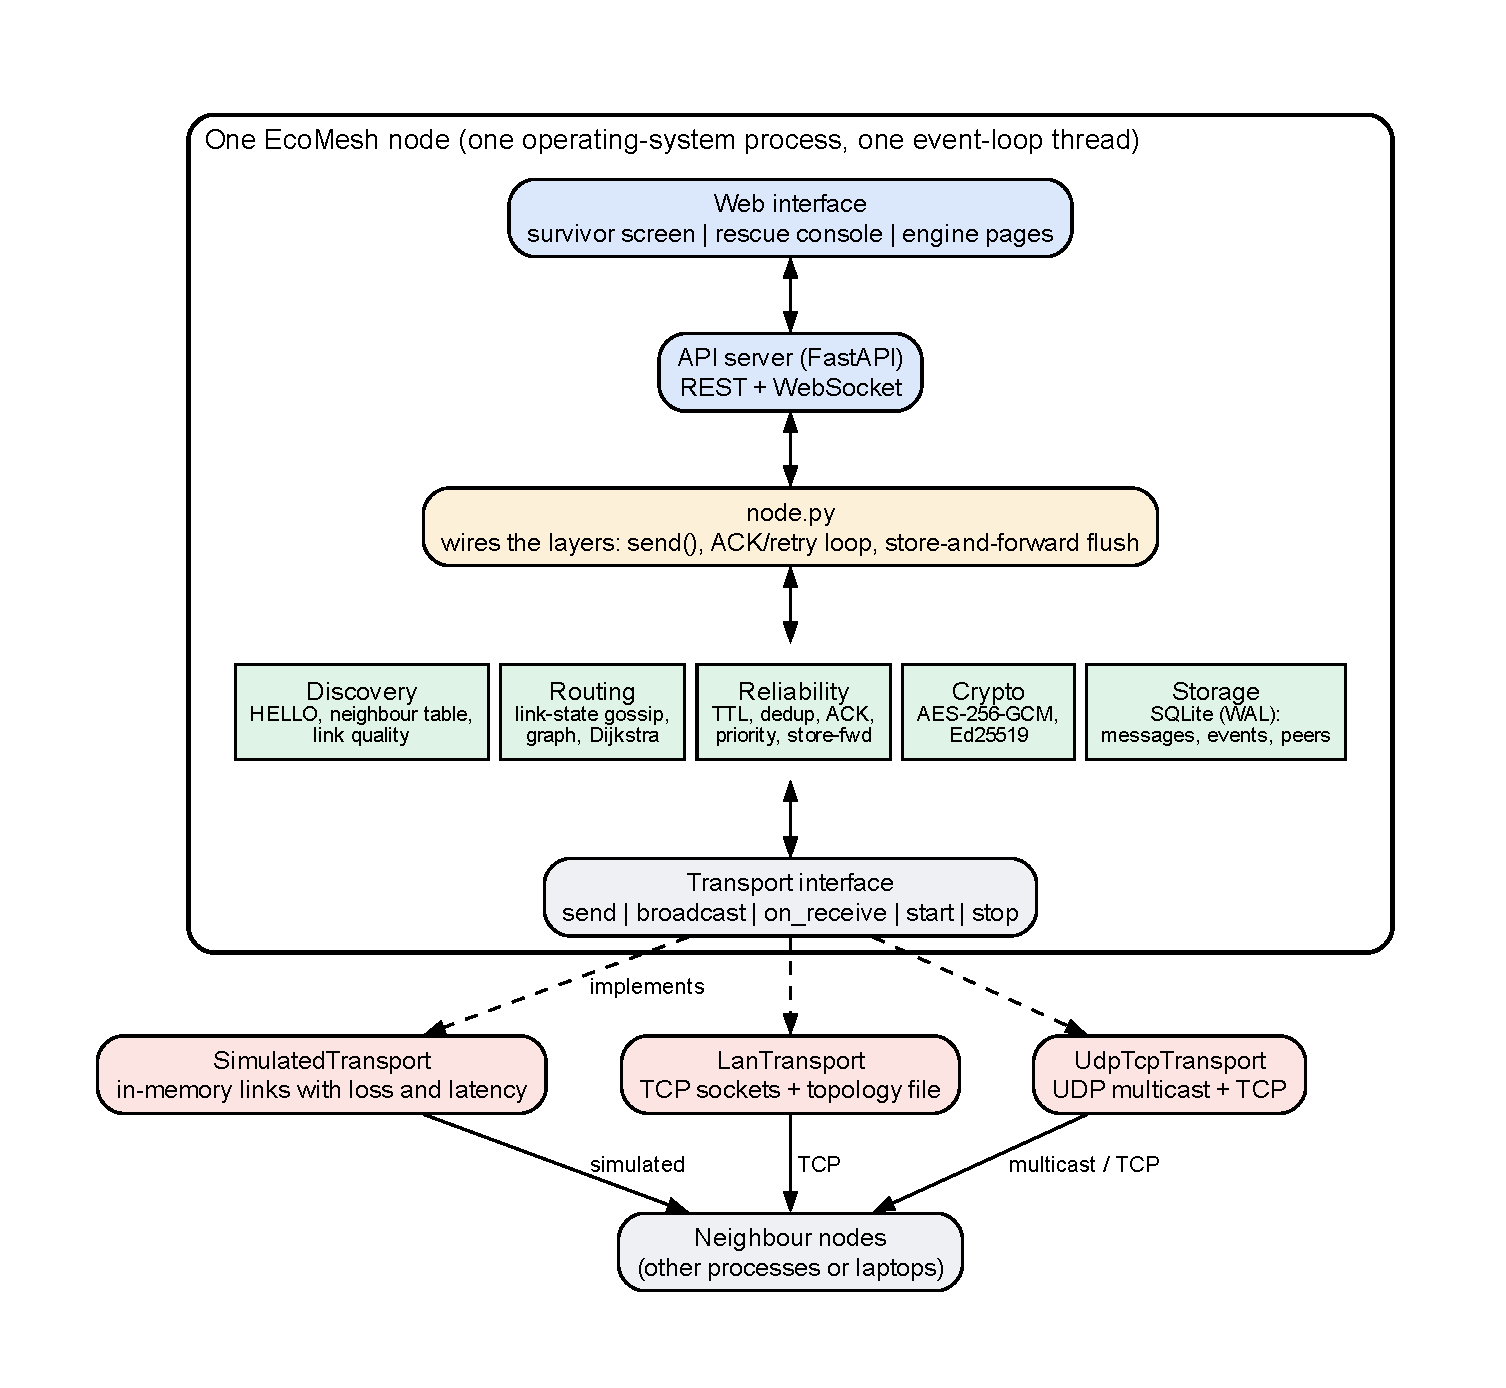
\includegraphics[width=0.72\textwidth]{figures/fig_architecture.pdf}
\caption{Block diagram: one EcoMesh node and its three interchangeable transports}
\label{fig:arch}
\end{figure}

\subsection{Component and Module Description}
The engine has one module per concern: \texttt{packet.py} (wire format), the transports, \texttt{discovery.py}, \texttt{routing.py}, \texttt{relay.py}, \texttt{reliability.py}, \texttt{crypto.py} and \texttt{store.py}, joined only in \texttt{node.py}. \texttt{sim/} and \texttt{api/} drive the engine for experiments, and \texttt{story/} serves the device screens. Table~\ref{tab:impl} in Section~\ref{sec:modules} gives each module's input and output, logic, dependencies and tests.

\textbf{Wire protocol.} A fixed big-endian header (Table~\ref{tab:header}) is followed by the path travelled so far, the payload and an optional 64-byte signature. The path is carried so that loops can be detected and the screens can show the route. HELLO is a one-hop broadcast, LINK\_STATE is sent to each neighbour, and DATA and ACK travel over TCP on each hop, so every hop is ordered and reliable even though the end-to-end path is not.
\begin{table}[!htbp]
\caption{The 52-byte packet header}
\label{tab:header}
\footnotesize
\setlength{\tabcolsep}{3.5pt}
\begin{tabular}{@{}rrll@{\hspace{8pt}}rrll@{}}
\toprule
\textbf{Off.} & \textbf{Size} & \textbf{Field} & \textbf{Meaning} & \textbf{Off.} & \textbf{Size} & \textbf{Field} & \textbf{Meaning}\\ \midrule
0 & 2 & magic & \texttt{0x4D45} ``ME'' & 24 & 8 & src & node id, ASCII\\
2 & 1 & version & 1 & 32 & 8 & dst & node id / \texttt{RESCUE\_\_}\\
3 & 1 & type & HELLO, LINK\_STATE, DATA, ACK & 40 & 8 & timestamp & Unix ms\\
4 & 1 & priority & 0 SOS, 1 NORMAL, 2 STATUS & 48 & 2 & payload\_len & bytes\\
5 & 1 & ttl & per-hop decrement (10) & 50 & 1 & path\_len & ids in path\\
6 & 1 & flags & enc., needs\_ack, s-f, signed & 51 & 1 & attempt & retry counter\\
7 & 1 & hop\_count & per-hop increment & 8 & 16 & msg\_id & UUIDv4\\
\bottomrule
\end{tabular}
\end{table}

\subsection{Architecture Selection and Justification}
\textbf{Layered and independent of the transport.} A single boundary separates moving bytes from everything else, which gives a deterministic simulator, unit tests without sockets and a direct answer to the missing radio: a Bluetooth transport would be one more implementation, not a rewrite. \textbf{One \texttt{asyncio} thread instead of several threads.} Four activities share three structures; on one loop they cannot race, so correctness does not depend on locking discipline. \textbf{Peer-to-peer instead of client--server.} A server would be a single point of failure and exactly the infrastructure that fails in a disaster. \textbf{Link state instead of flooding or on-demand discovery.} Flooding breaks down under load, and discovering a route on demand delays the first emergency packet. \textbf{SQLite per node in WAL mode.} It is a file with no server, and the API can read while the engine writes.

\subsection{Data Flow Diagram (DFD)}
Figure~\ref{fig:dfd0} is the context diagram (one node, no server); Figure~\ref{fig:dfd1} splits the node into six processes and five data stores.
\begin{figure}[!htbp]
\centering
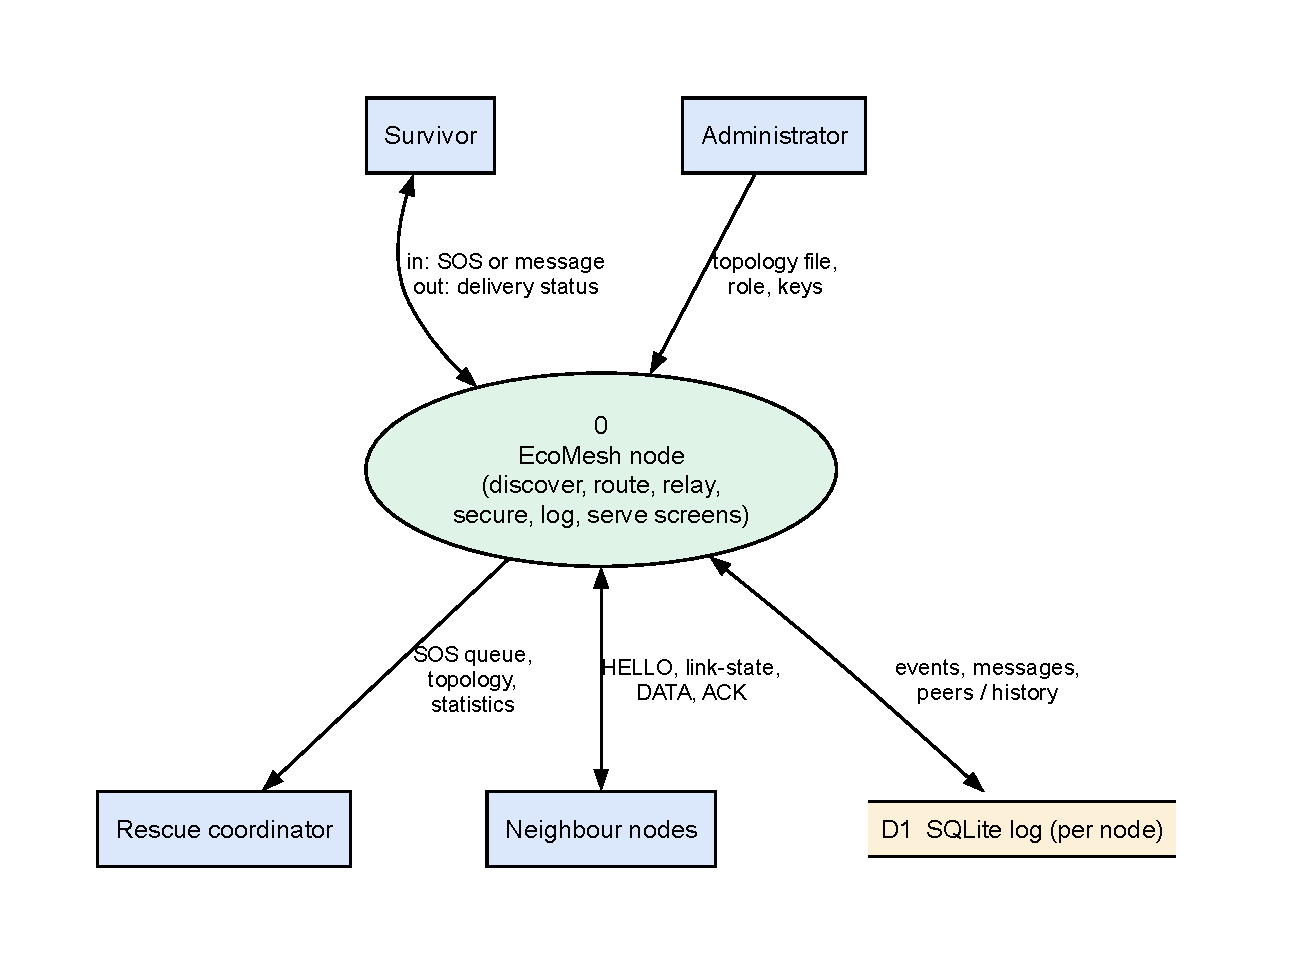
\includegraphics[width=0.5\textwidth]{figures/fig_dfd0.pdf}
\caption{Level-0 (context) data flow diagram}
\label{fig:dfd0}
\end{figure}
\begin{figure}[!htbp]
\centering
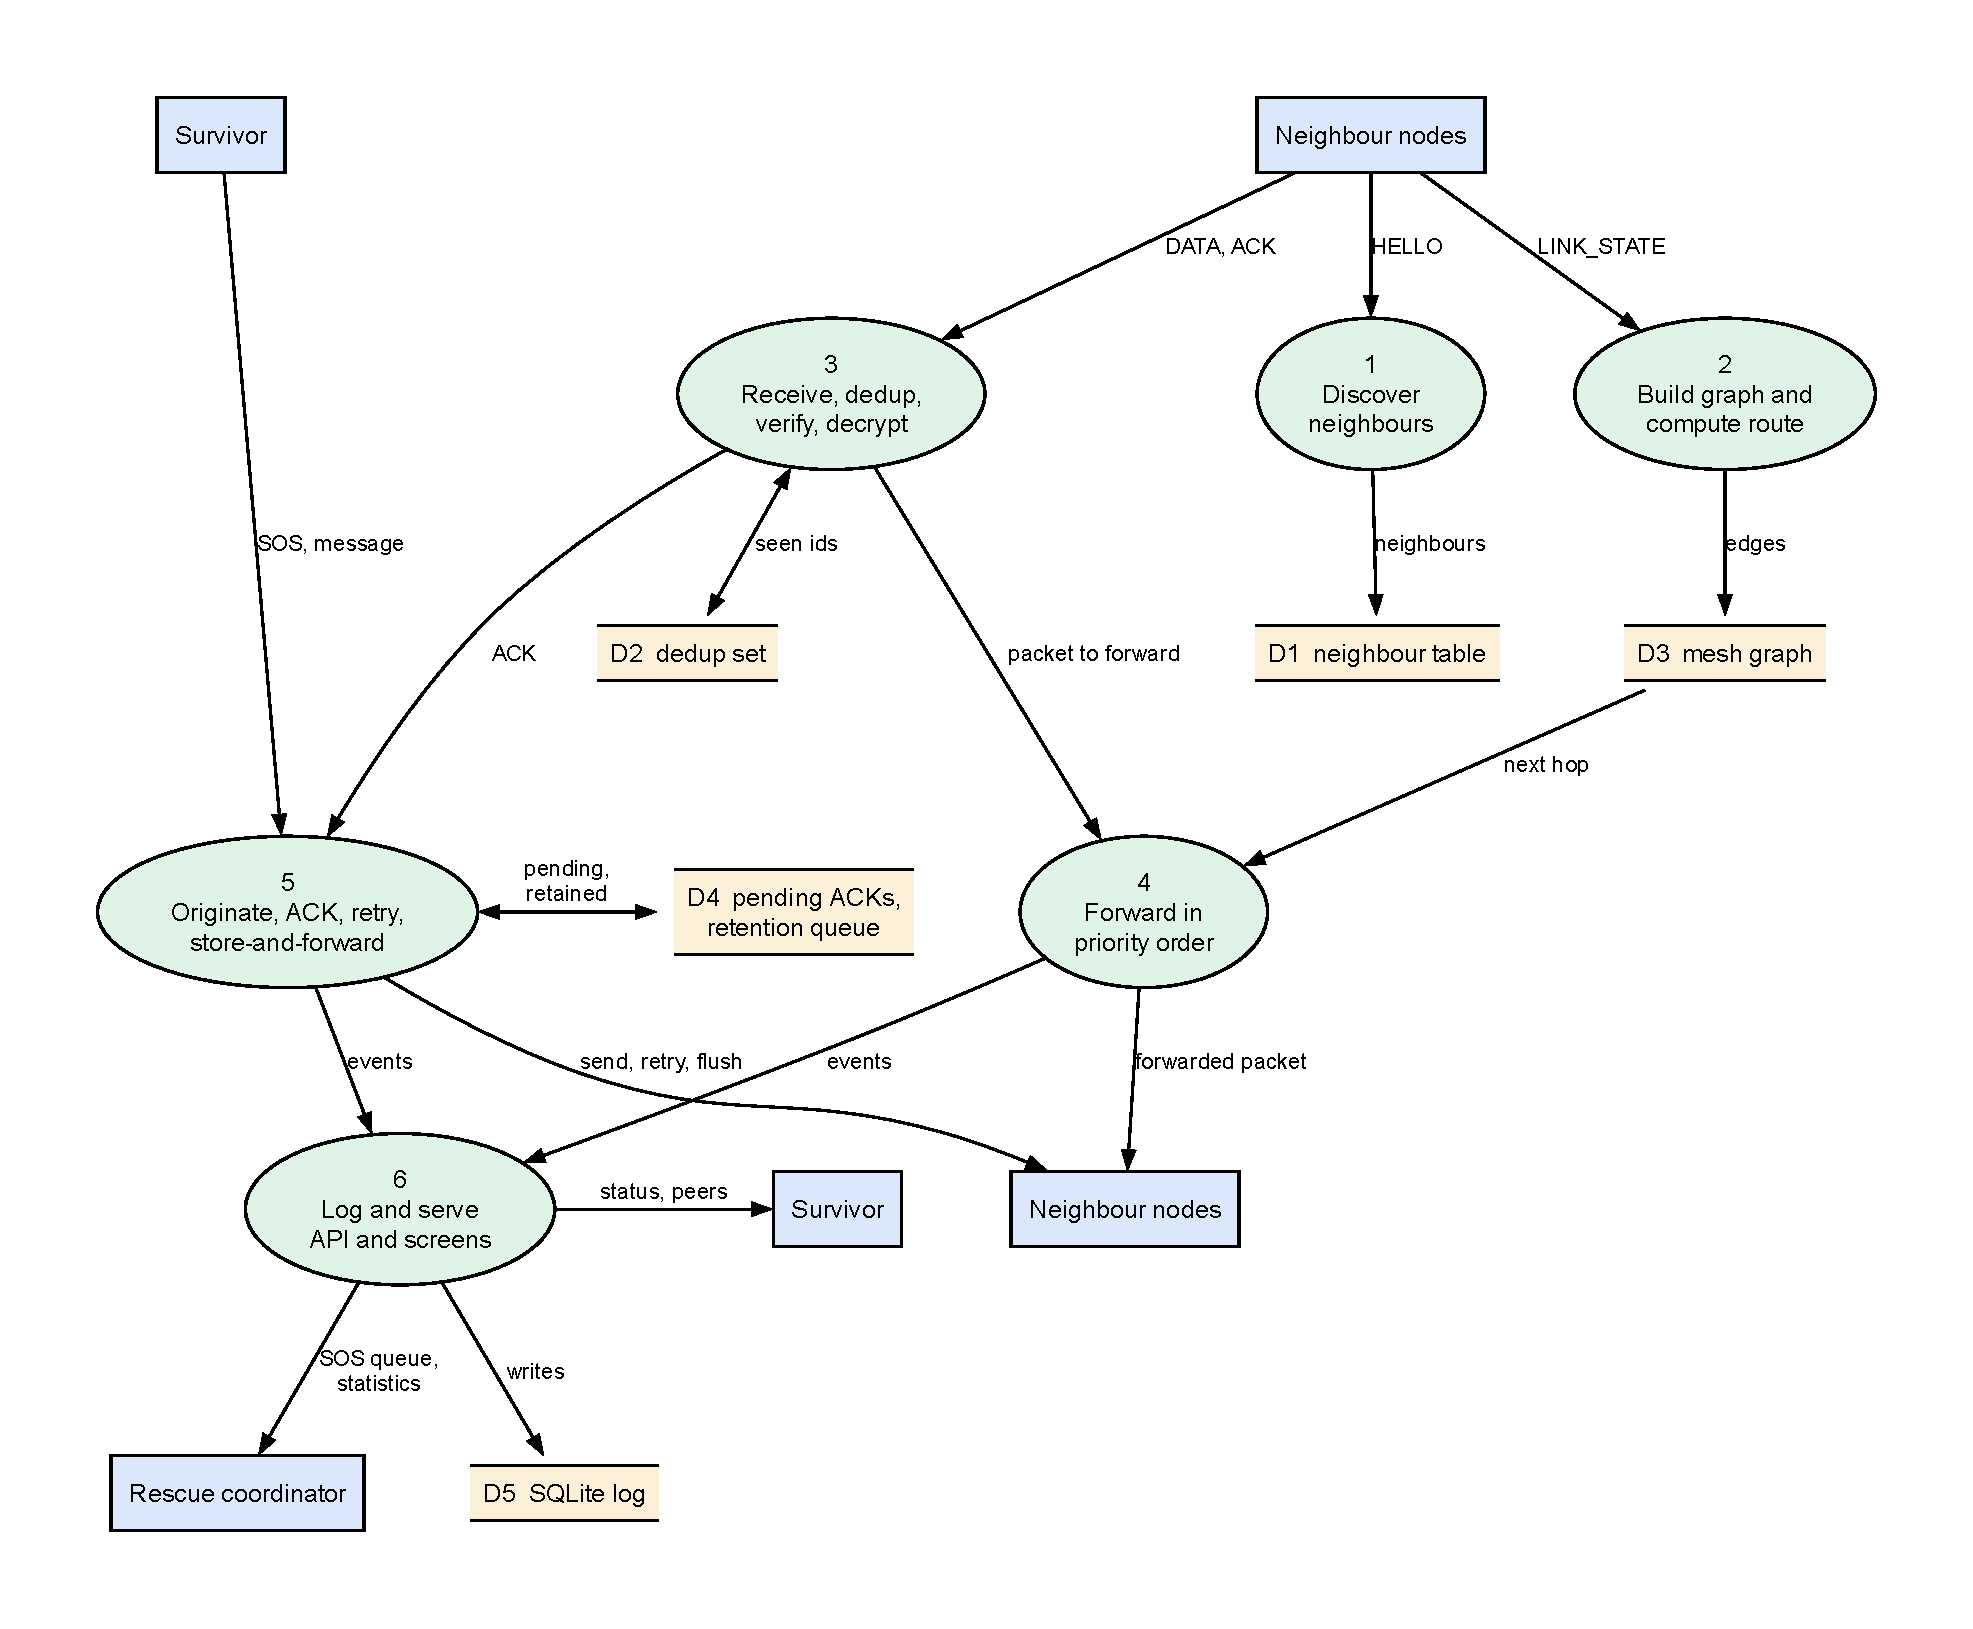
\includegraphics[width=\textwidth,height=0.52\textheight,keepaspectratio]{figures/fig_dfd1.pdf}
\caption{Level-1 data flow diagram of one node}
\label{fig:dfd1}
\end{figure}

\subsection{UML Diagrams}
The six UML diagrams of Phase~II match the implemented design. \textbf{Use case diagram} (Figure~\ref{fig:usecase}): five actors; raising an SOS includes sending a message, and holding and flushing extends sending when there is no route.
\begin{figure}[!htbp]
\centering
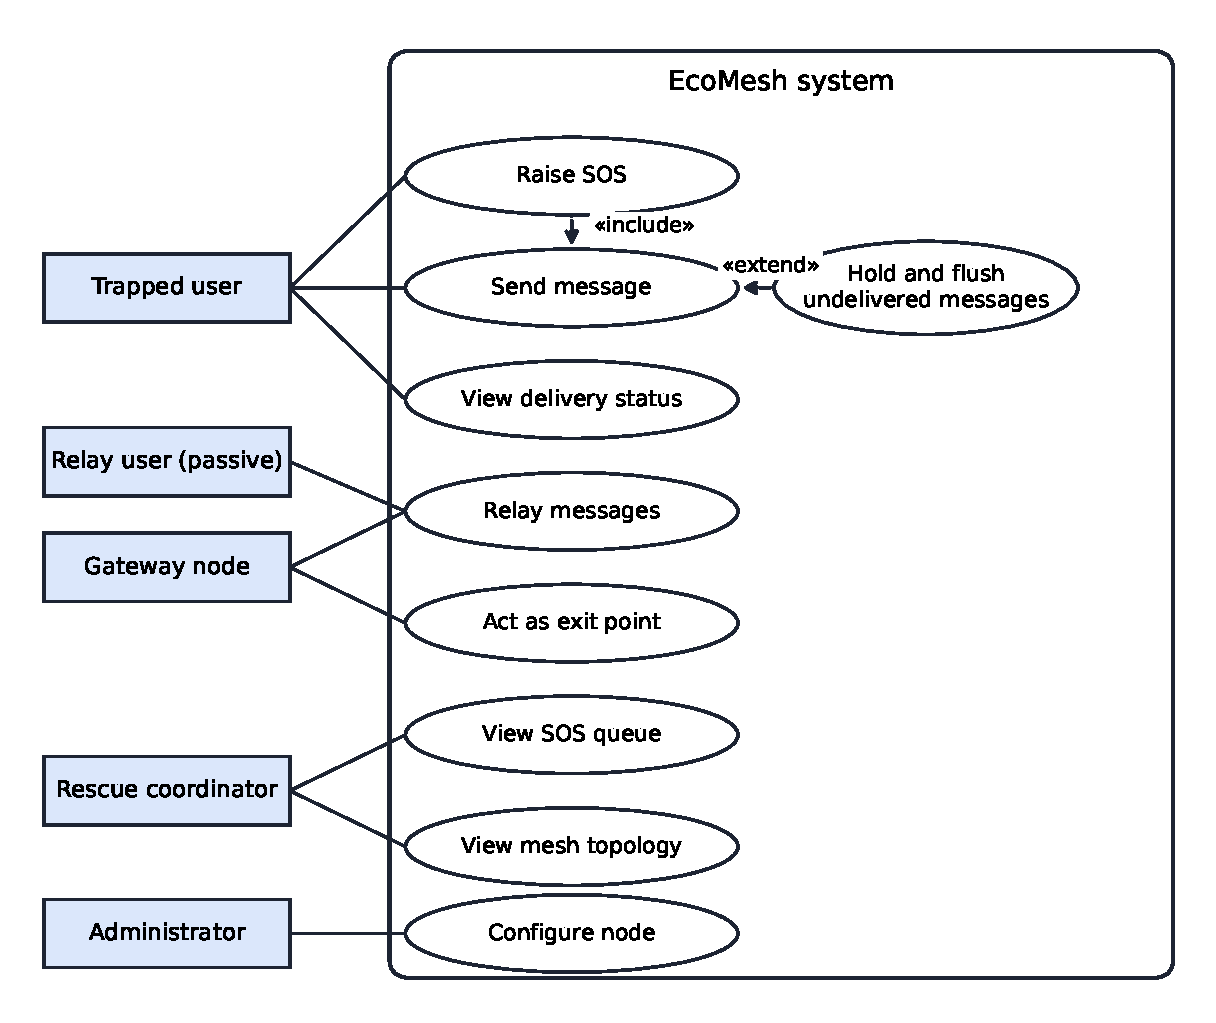
\includegraphics[width=0.62\textwidth]{figures/uml_usecase.pdf}
\caption{Use case diagram}
\label{fig:usecase}
\end{figure}
\textbf{Class diagram} (Figure~\ref{fig:class}). \texttt{Node} owns the discovery, gossip, routing, relay, ACK-tracking, retention and storage objects (filled diamonds); the router and the gossip share one \texttt{MeshGraph}; the relay owns its priority queue and uses a duplicate set; three classes implement \texttt{Transport}. \textbf{Activity diagram} (Figure~\ref{fig:activity}). An arriving packet is validated and checked for duplicates. If it is addressed to this node, its signature is verified and its payload decrypted, and it is logged, acknowledged and delivered; otherwise the TTL, loop and route checks decide whether it is dropped or queued again by priority.
\begin{figure}[!htbp]
\centering
\begin{minipage}[b]{0.49\textwidth}\centering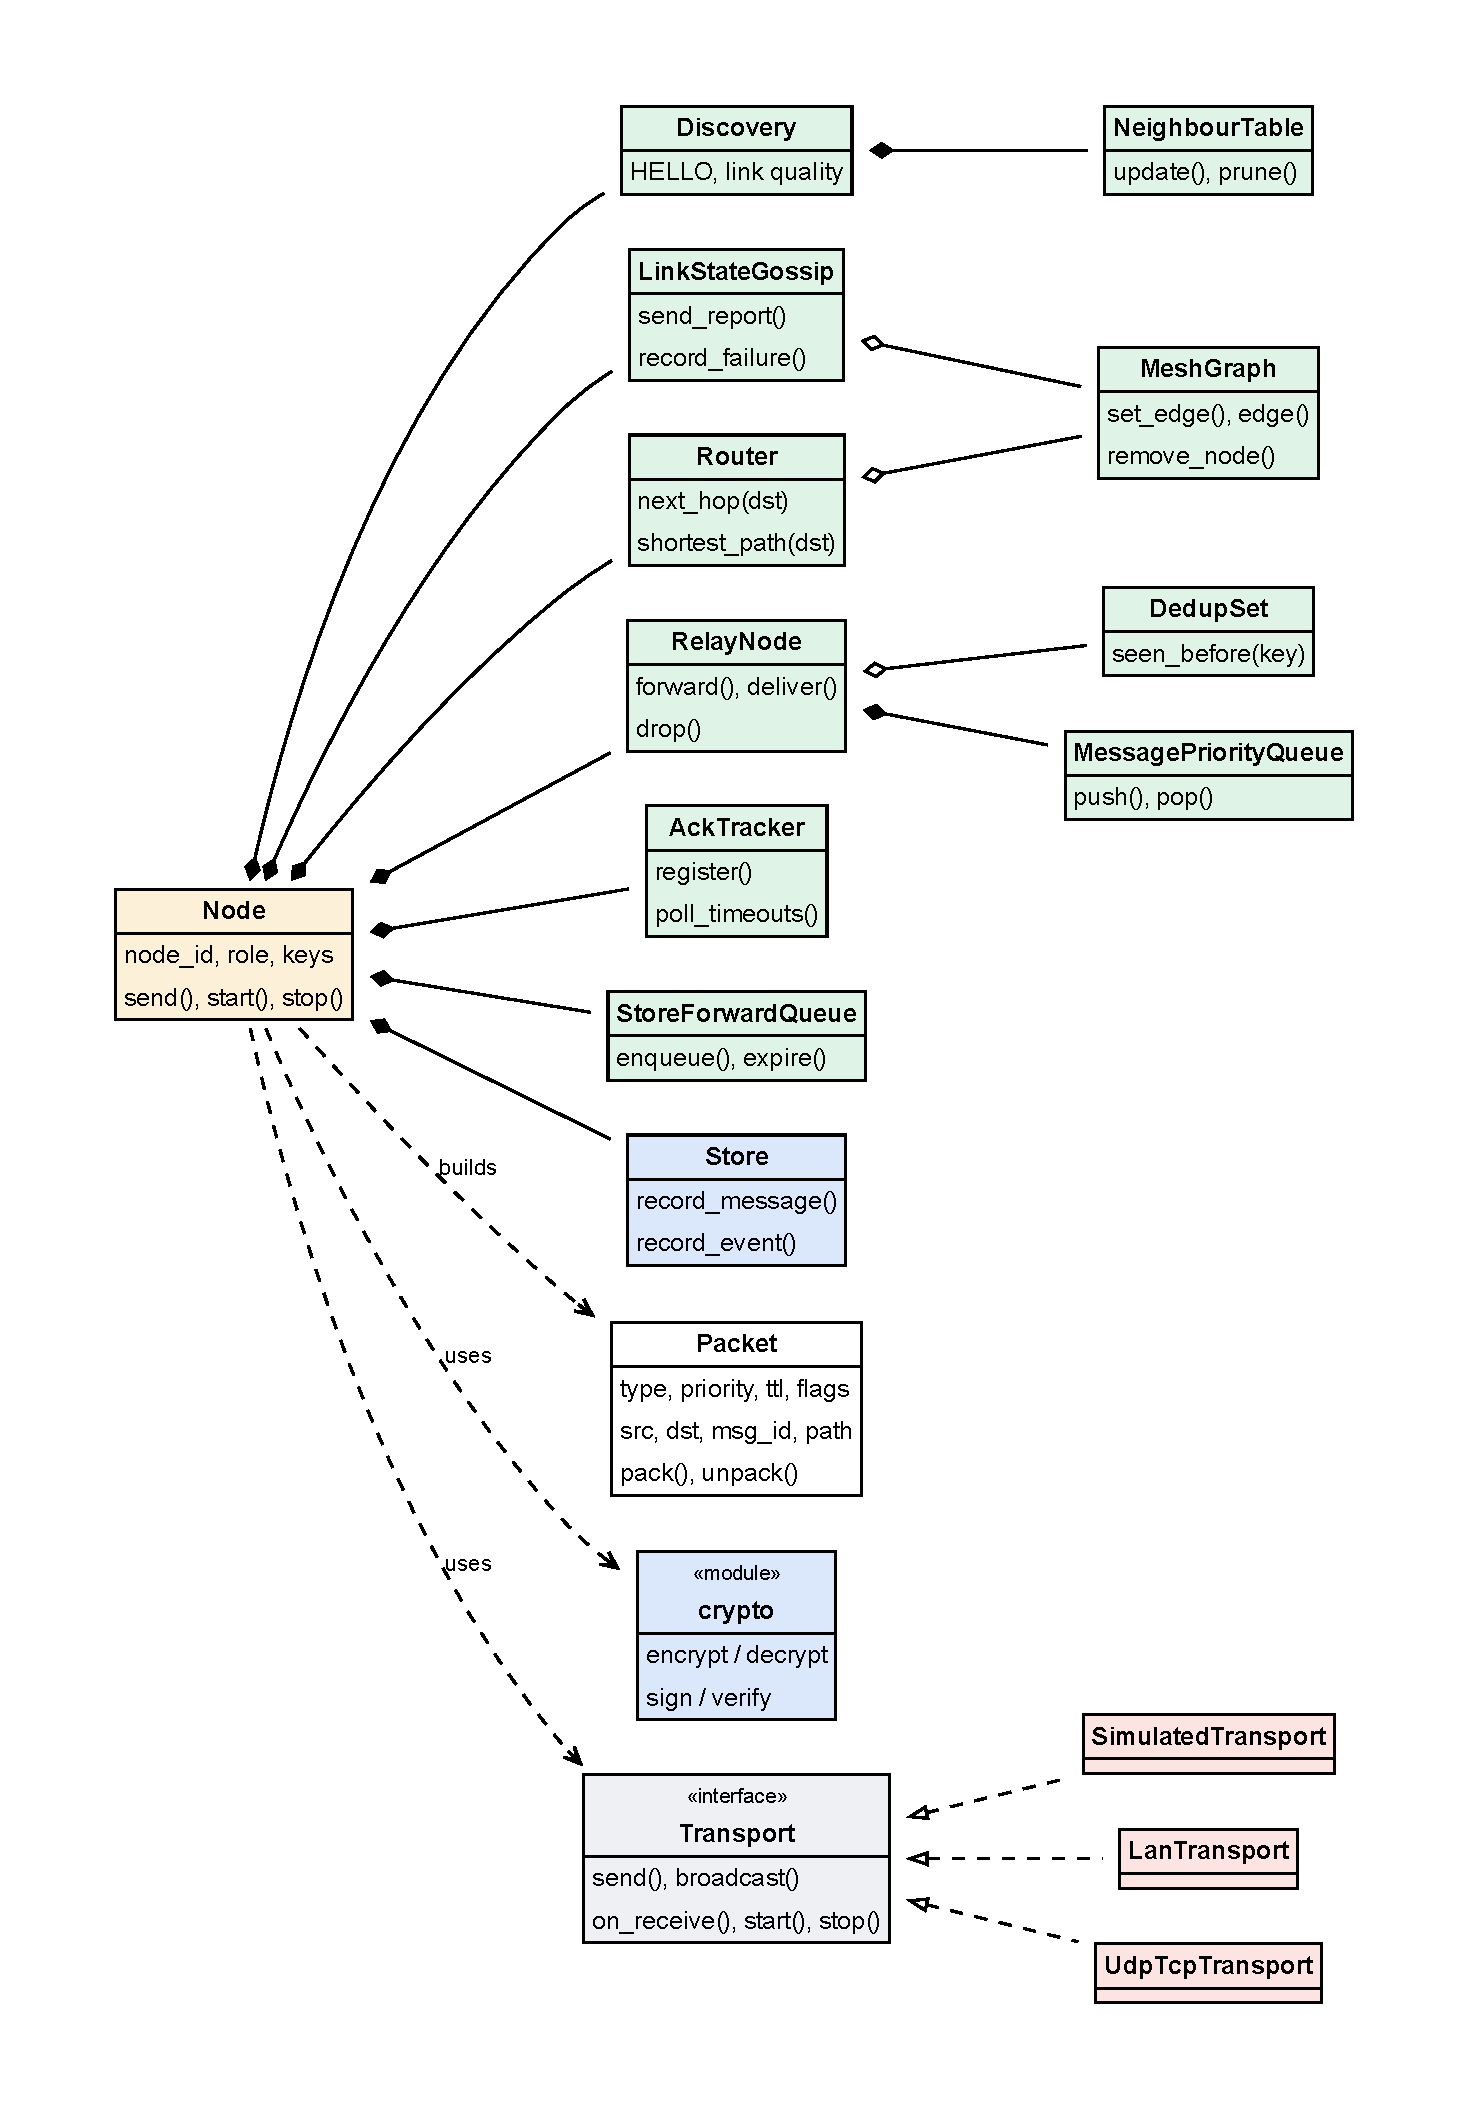
\includegraphics[width=\linewidth,height=0.49\textheight,keepaspectratio]{figures/uml_class.pdf}
\captionof{figure}{Class diagram: \texttt{Node} as the composition root}\label{fig:class}\end{minipage}\hfill
\begin{minipage}[b]{0.49\textwidth}\centering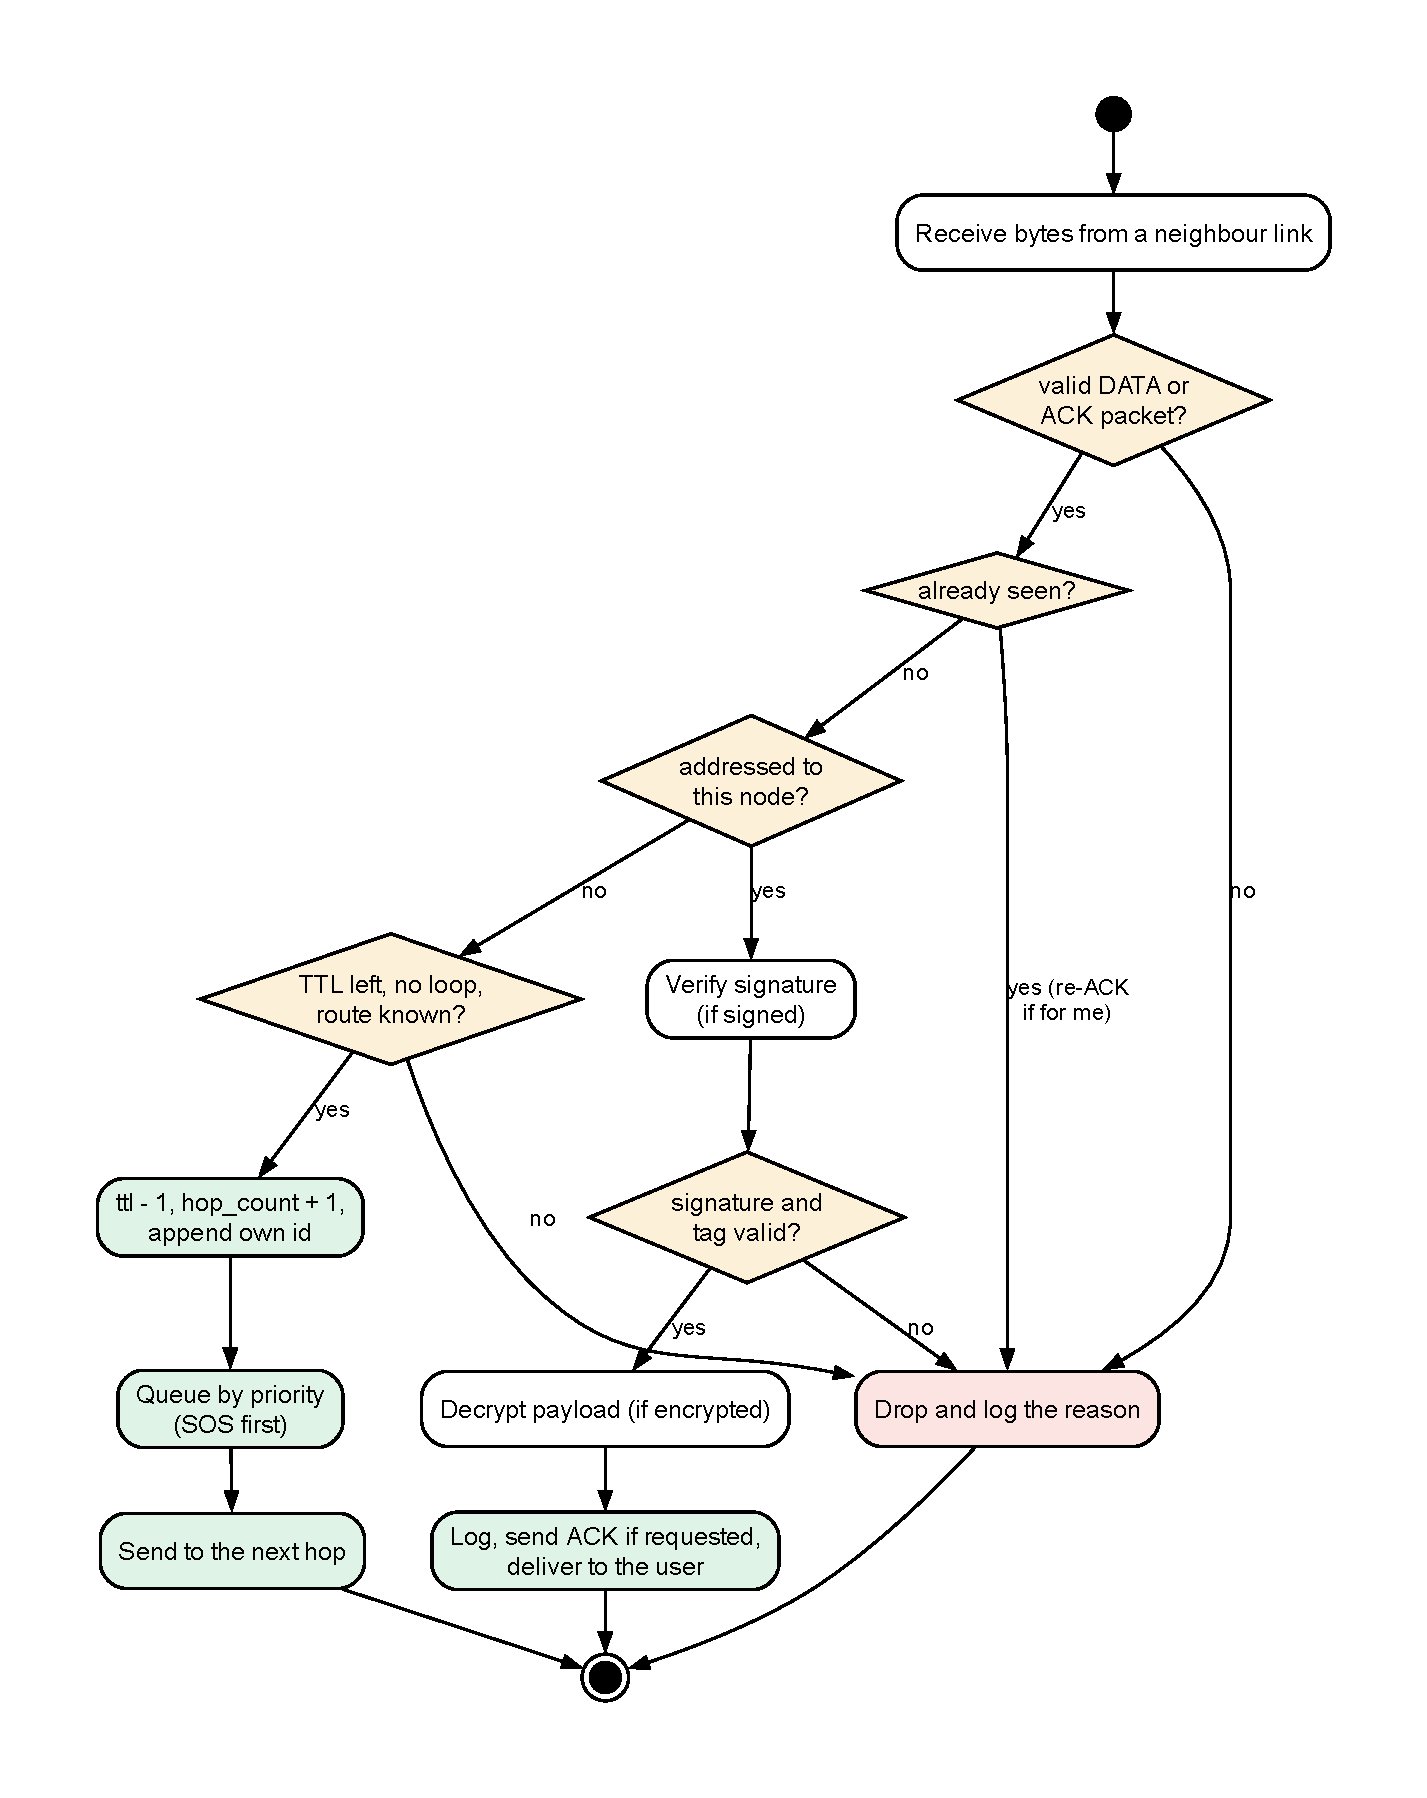
\includegraphics[width=\linewidth,height=0.49\textheight,keepaspectratio]{figures/uml_activity.pdf}
\captionof{figure}{Activity diagram: the packet receive path}\label{fig:activity}\end{minipage}
\end{figure}
\textbf{Sequence diagram} (Figure~\ref{fig:sequence}). L1 creates, encrypts and signs an SOS; each relay checks duplicates, lowers the TTL and adds its id; L5 delivers it and the ACK returns.
\begin{figure}[!htbp]
\centering
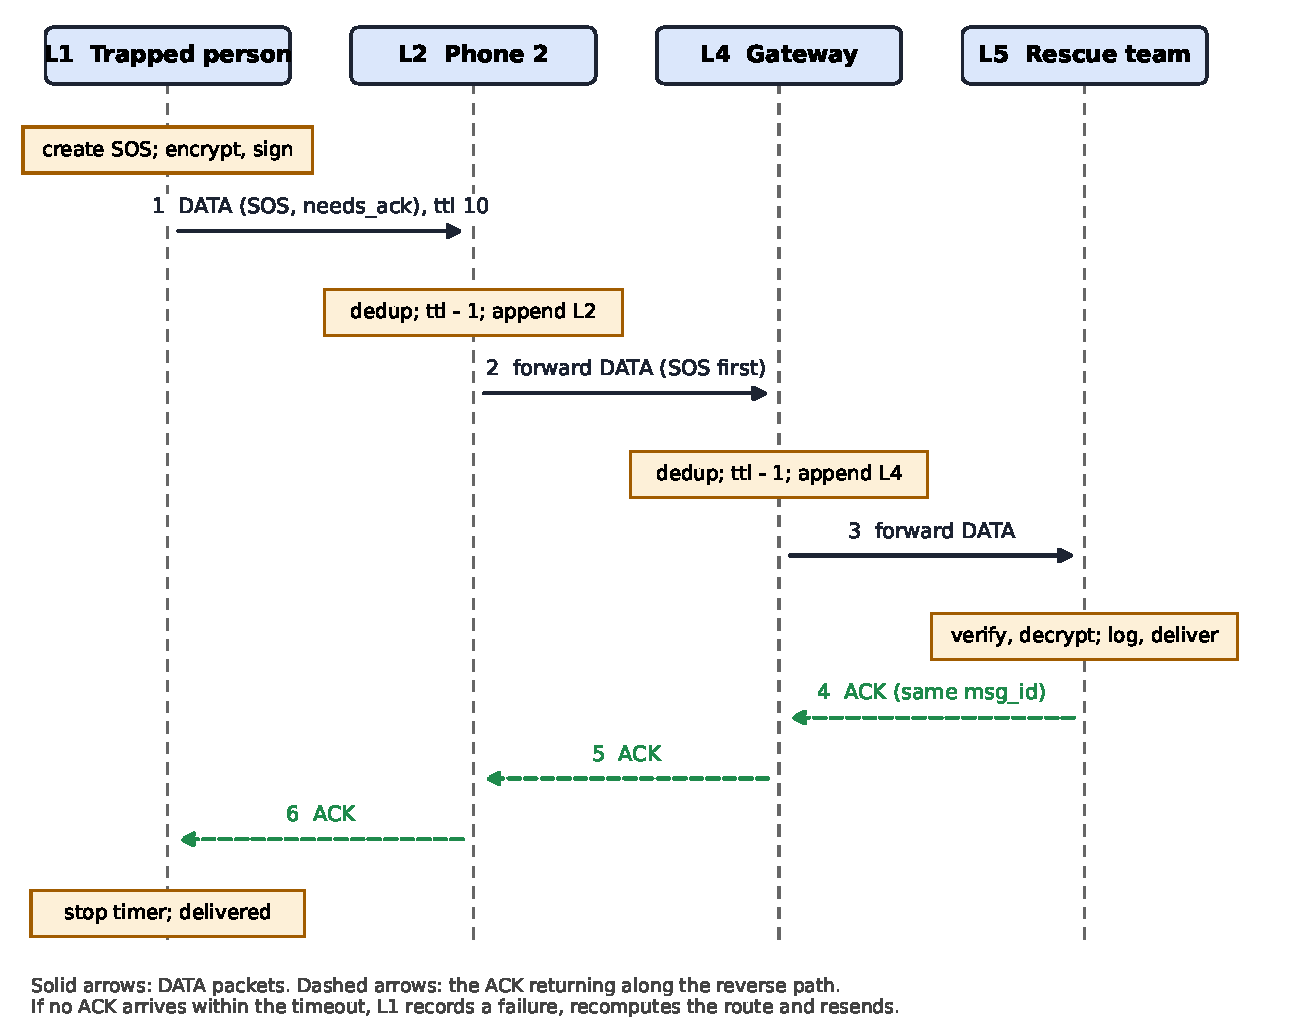
\includegraphics[width=0.82\textwidth]{figures/uml_sequence.pdf}
\caption[Sequence diagram: an SOS relayed hop by hop]{Sequence diagram: an SOS relayed hop by hop with the ACK returning along the reverse path}
\label{fig:sequence}
\end{figure}
\textbf{State machine} (Figure~\ref{fig:state}, left). A message is created, becomes pending (sent and awaiting an ACK) or held (no route), and ends delivered or failed; these states are the \texttt{status} values stored in the database. \textbf{Deployment diagram} (Figure~\ref{fig:deploy}, right). Five node processes, each with its own engine, web screen and SQLite file, connected only by the TCP links that the topology file lists; there is no server (Section~\ref{sec:lan}).
\begin{figure}[!htbp]
\centering
\begin{minipage}[b]{0.52\textwidth}\centering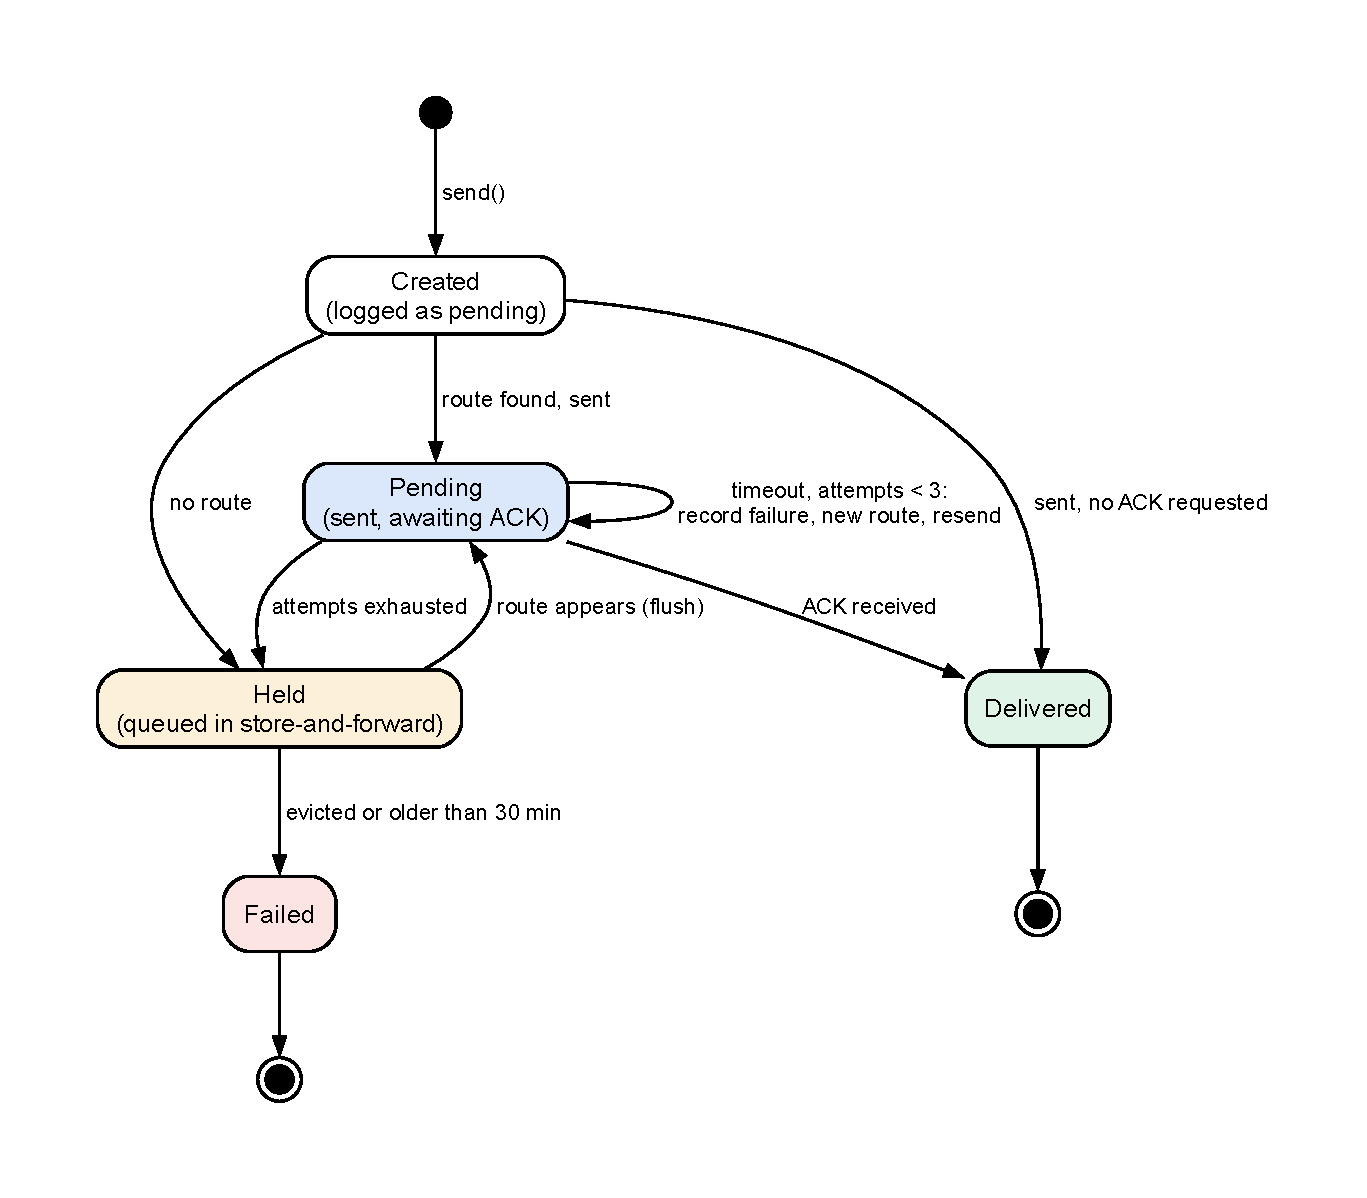
\includegraphics[width=\textwidth]{figures/uml_state.pdf}\end{minipage}\hfill
\begin{minipage}[b]{0.36\textwidth}\centering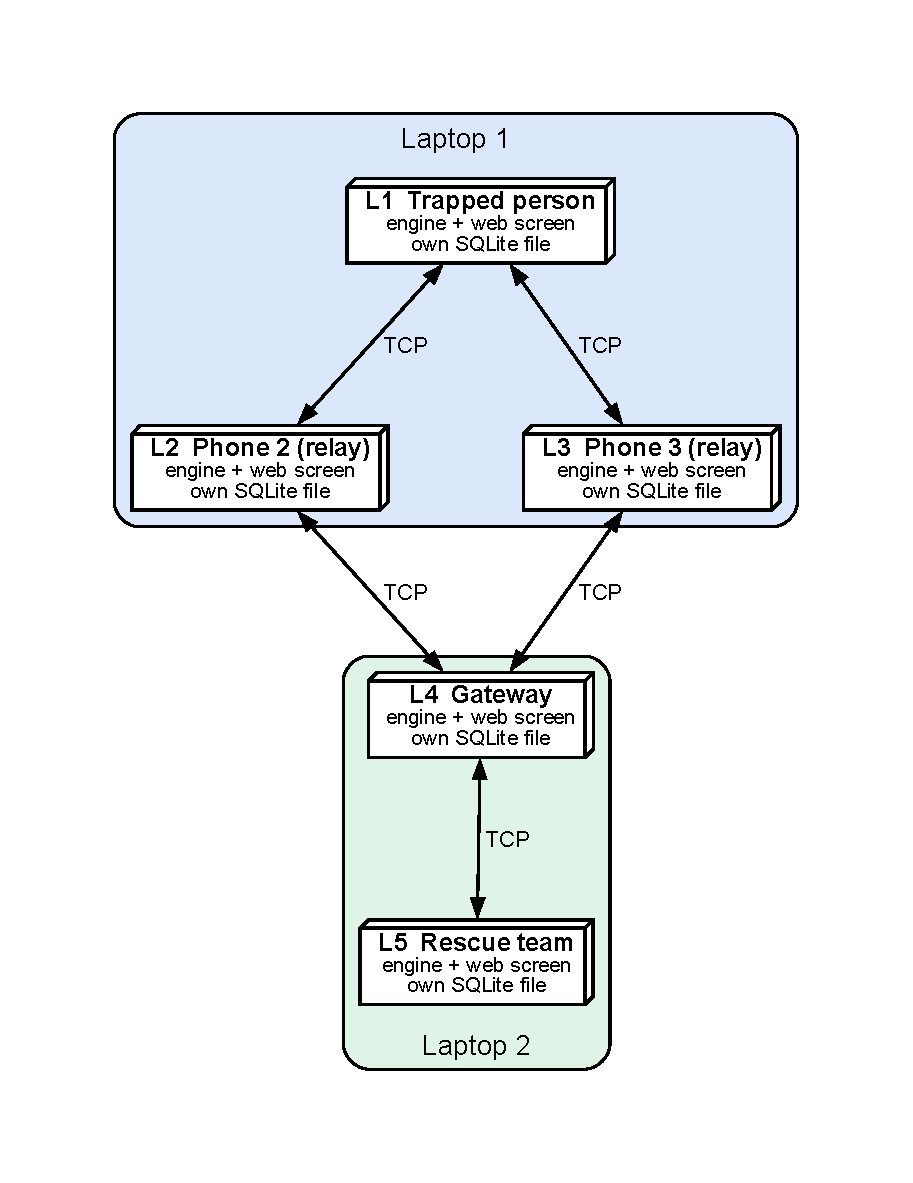
\includegraphics[width=\textwidth]{figures/uml_deploy.pdf}\end{minipage}
\caption[State machine of the message lifecycle and deployment diagram]{State machine of the message lifecycle (left) and deployment diagram of the live configuration (right)}
\label{fig:state}\label{fig:deploy}
\end{figure}

\subsection{Database Design}
\label{sec:db}
Every node keeps its own SQLite database in WAL mode, accessed with plain \texttt{sqlite3} and SQL; with only three tables an ORM would add indirection and nothing else. Every metric is a query over this database (SRS 6.1).
\begin{figure}[!htbp]
\centering
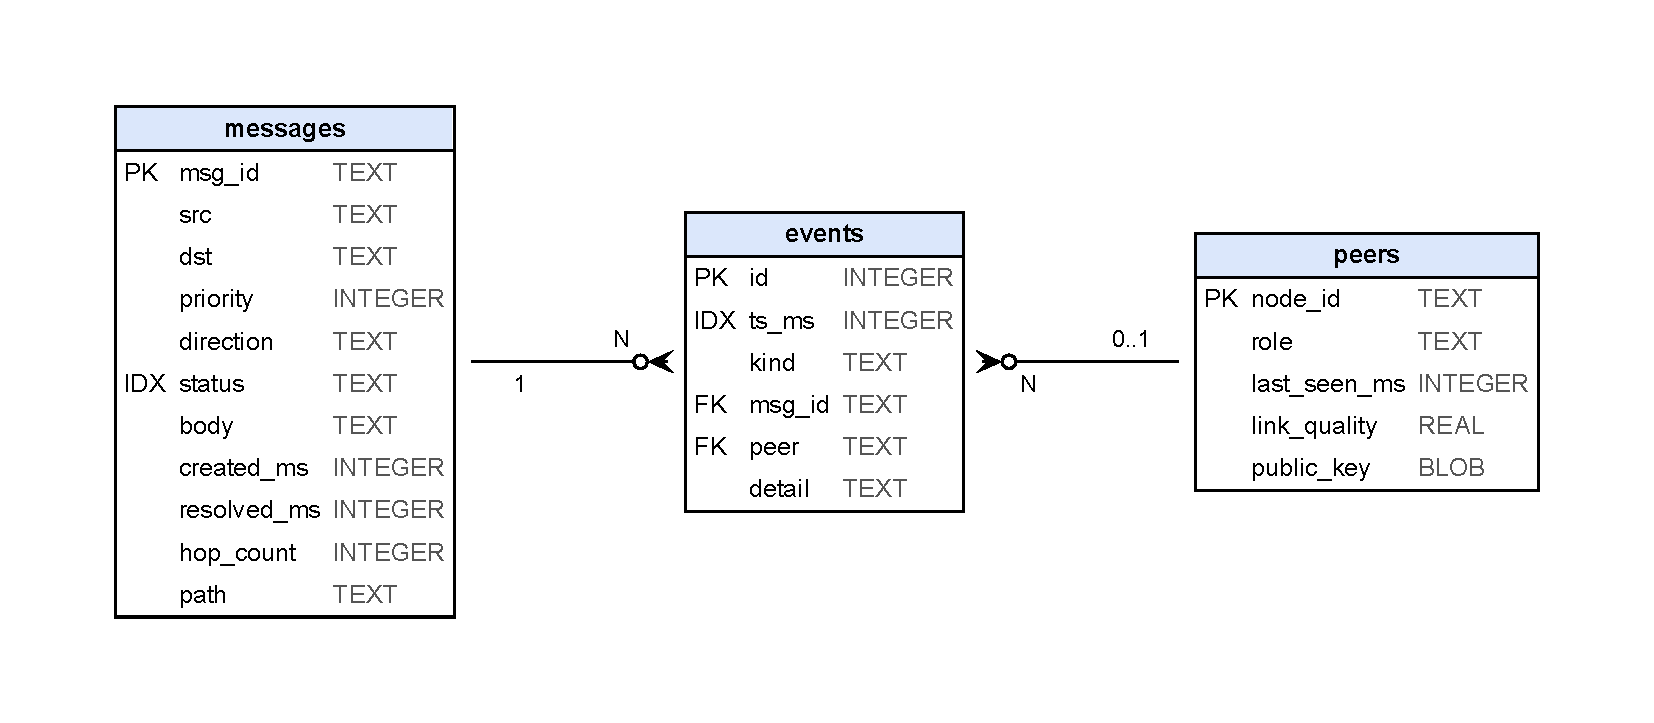
\includegraphics[width=0.92\textwidth]{figures/fig_er.pdf}
\caption[Entity--relationship diagram of the per-node database]{Entity--relationship diagram of the per-node database (PK primary key, IDX secondary index, FK logical foreign key)}
\label{fig:er}
\end{figure}
\textbf{Relational schema.} \texttt{messages}(\texttt{msg\_id} PK, \texttt{src}, \texttt{dst}, \texttt{priority}, \texttt{direction} in sent/received/forwarded, \texttt{status} in pending/delivered/failed/queued\_sf, \texttt{body}, \texttt{created\_ms}, \texttt{resolved\_ms}, \texttt{hop\_count}, \texttt{path}); \texttt{events}(\texttt{id} PK, \texttt{ts\_ms}, \texttt{kind}, \texttt{msg\_id}, \texttt{peer}, \texttt{detail}); \texttt{peers}(\texttt{node\_id} PK, \texttt{role}, \texttt{last\_seen\_ms}, \texttt{link\_quality}, \texttt{public\_key}). \textbf{Keys and integrity.} The UUID \texttt{msg\_id} joins messages to events; \texttt{body} holds plaintext only at source and destination; upserts move a message from pending to queued\_sf to delivered in one row; \texttt{events.msg\_id} and \texttt{events.peer} are logical foreign keys, since a relay logs events for messages it never stores. \textbf{Normalisation.} Third normal form, except the comma-separated \texttt{path}, always read whole. \textbf{Indexing.} \texttt{idx\_events\_ts} serves the live panel and \texttt{idx\_msg\_status} the held-message count. \textbf{Sample records} are in Table~\ref{tab:samples}; the relay's row has no body.
\begin{table}[htbp]
\caption{Sample rows of \texttt{messages} for one SOS from A to C in a real run: each node holds its own view of the same message id}
\label{tab:samples}
\footnotesize
\setlength{\tabcolsep}{3pt}
\begin{tabular}{@{}llllllllll@{}}
\toprule
\textbf{DB} & \textbf{msg\_id} & \textbf{src} & \textbf{dst} & \textbf{prio} & \textbf{direction} & \textbf{status} & \textbf{body} & \textbf{hops} & \textbf{path} \\ \midrule
A & 8e859198... & A & C & 0 & sent & delivered & trapped on floor 3 & 1 & B \\
B & 8e859198... & A & C & 0 & forwarded & delivered & NULL & 1 & B \\
C & 8e859198... & A & C & 0 & received & delivered & trapped on floor 3 & 1 & B \\
\bottomrule
\end{tabular}
\end{table}


\subsection{Security and Error Handling Design}
\label{sec:secdesign}
Table~\ref{tab:threat} links each threat to its countermeasure and requirement.
\begin{table}[!htbp]
\caption{Threat model and countermeasures}
\label{tab:threat}
\footnotesize
\begin{tabularx}{\textwidth}{@{}>{\raggedright\arraybackslash}p{4.0cm}>{\raggedright\arraybackslash}X>{\raggedright\arraybackslash}p{2.6cm}@{}}
\toprule
\textbf{Threat} & \textbf{Mechanism} & \textbf{Requirement}\\ \midrule
Relay reads a message & AES-256-GCM payload; relays see only routing fields & SEC-1, 2, FWD-7\\
Relay modifies a message & GCM tag fails at the destination; dropped, logged & SEC-5\\
Relay forges an SOS & Ed25519 signature over the identity fields & SEC-3, 4, 6\\
Replay of a captured packet & dedup set keyed on message id (300\,s) & REL-3\\
Malformed or hostile bytes & strict validation; \texttt{PacketError}; drop & FWD-6\\
Endless circulation & TTL per hop; own id in the path is a loop & FWD-3, 5\\
Hand-rolled cryptography & only \texttt{cryptography}-library primitives & SEC-7\\
\bottomrule
\end{tabularx}
\end{table}
\textbf{Authentication.} A node's identity is its Ed25519 key pair, announced in HELLO and gossip. \textbf{Authorisation.} Only GATEWAY and RESCUE nodes accept \texttt{RESCUE\_\_} traffic; any node may relay but never decrypts or stores what it does not own. One pre-shared key covers the mesh, so a node holding it could read what it forwards; per-pair keys would prevent this (Section~\ref{sec:limits}). \textbf{Input validation and exceptions.} Every field is range-checked; a violation raises \texttt{PacketError} and the packet is dropped and logged, never raised into the event loop; \texttt{verify} returns \texttt{False} instead of raising. \textbf{Logging.} Each drop has its own event (\texttt{drop\_ttl}, \texttt{drop\_loop}, \ldots). \textbf{Sensitive data.} Fresh 12-byte nonces; plaintext only at the two ends; private keys never sent; the signature skips fields that change in transit (TTL, hops, path).

\section{Algorithm Design and Data Structures}
\label{ch:alg}

\subsection{Identification of Critical Operations}
Ten operations decide correctness and performance: (1) neighbour discovery and link-quality estimation; (2) link-state dissemination; (3) least-cost route computation; (4) the per-packet forwarding decision; (5) priority scheduling; (6) duplicate suppression; (7) send, acknowledge and retry; (8) bounded store-and-forward; (9) encryption and signing; (10) resolution of the symbolic destination \texttt{RESCUE\_\_}. They correspond to Algorithms 1--10 of the Phase~II \emph{Design of Algorithms}; the pseudocode below reflects the implemented code, including the Phase~4 corrections.

\subsection{Algorithm Design}
\label{sec:algdesign}
\textbf{A1 Discovery and link quality.}
\begin{lstlisting}
every 3 s: broadcast HELLO(role, public_key)                      // ttl = 1
on HELLO from p:  new <- table.update(p);  if new: on_peer_up(p)
    q <- hellos_received / hellos_expected   in a 20-slot window    // in [0,1]
    if |q - last_reported| >= 0.1: report q                         // avoids recomputing on noise
every 1 s: for p silent > 10 s: remove p; on_peer_down(p)
\end{lstlisting}
A new neighbour is scored over the HELLOs \emph{due} so far, otherwise every fresh link would look lossy. (The Phase~II write-up planned a 10-slot window; the code uses 20.)

\textbf{A2 Link-state with re-flooding.}
\begin{lstlisting}
every 5 s: seq++; send report(origin=me, seq, [(p, q, failures, role, key) for p in neighbours]) to each neighbour
on report(origin, s, entries) from sender:
    if origin = me or s <= seq_seen[origin]: return                  // stale or own: stop
    seq_seen[origin] <- s;  replace origin's outgoing edges with entries;  learn roles and keys
    if changed: invalidate route cache
    forward report unchanged to every neighbour except origin and sender   // controlled re-flooding
\end{lstlisting}
Without re-flooding a node knows only its neighbours' neighbours; sequence numbers admit each report once per link, so flooding terminates.

\textbf{A3 Dijkstra and the cost function.}\label{sec:cost}
\begin{lstlisting}
cost(u->v) = 1 + 5 * (1 - q) + 3 * f        // f = ACK timeouts on the link in the last 60 s
dist[src] <- 0; heap <- {(0, src)}
while heap: (d,u) <- pop_min; if u visited: continue; mark u
    for (v, e) in graph.neighbours(u): if d + cost(e) < dist[v]: dist[v] <- d + cost(e); prev[v] <- u; push
next_hop(dst) = path[1] of the cached shortest path, or none (=> store-and-forward)
\end{lstlisting}
\textbf{Derivation of the coefficients.} The base 1 is the per-hop penalty; it keeps every weight positive (Dijkstra's condition) and prefers fewer hops between equal links. The term $5(1-q)$ makes loss expensive: a link delivering 40\,\% of its HELLOs costs $1+5(0.6)=4.0$, more than two clean hops (2.0) or three (3.0), which is exactly where minimum-hop routing errs (Figure~\ref{fig:cost}). The term $3f$ is steeper than the estimated-loss term because an ACK timeout is \emph{observed} failure: one adds the cost of three extra clean hops, and it applies at once so the retry avoids the failing link.
\begin{figure}[!htbp]
\centering
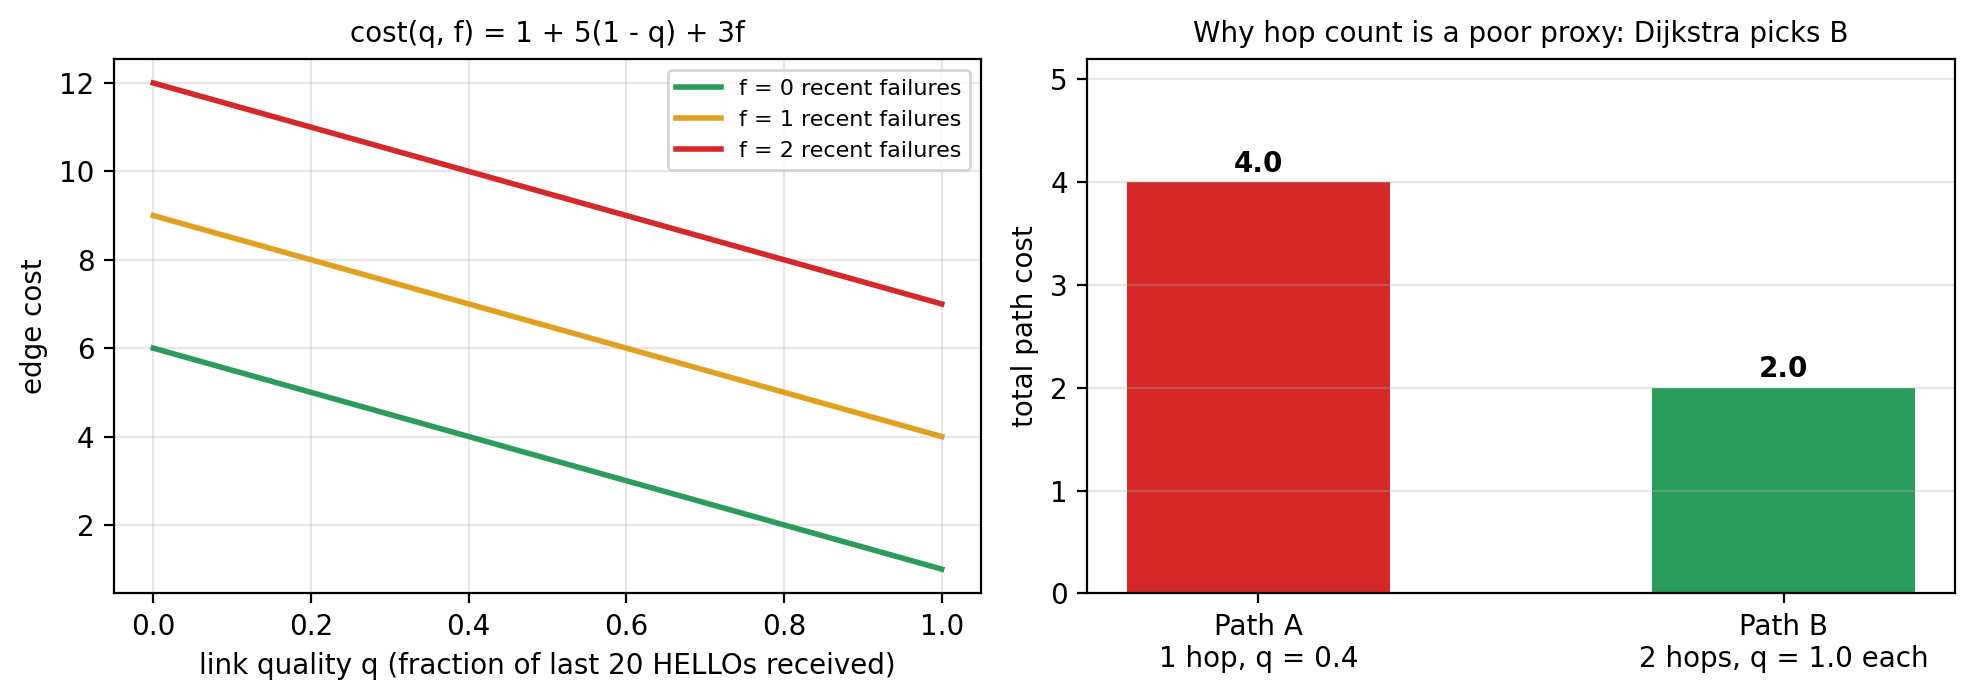
\includegraphics[width=0.5\textwidth]{figures/fig_cost.png}
\caption{The cost function, and why hop count is a poor proxy for delivery}
\label{fig:cost}
\end{figure}

\textbf{A4 Packet handling.}
\begin{lstlisting}
on packet p from link sender s:
    if not parse_ok(p) or p.type not in {DATA, ACK}: drop
    for_me <- p.dst = me or (p.dst = RESCUE__ and my role in {GATEWAY, RESCUE})
    key <- (type, msg_id) if for_me else (type, msg_id, attempt)     // a retry crosses relays that saw the original
    if dedup.seen_before(key): drop(duplicate); re-ACK if for_me; return
    if for_me: verify signature; decrypt; log; ACK if needs_ack; deliver
    elif ttl <= 0: drop(ttl_expired)   elif me in path: drop(loop)   elif no next_hop: drop(no_route)
    else: ttl--; hop_count++; path.append(me); queue.push(p, priority)            // A5
\end{lstlisting}
The key includes the \emph{type} because an ACK carries the id of the DATA it acknowledges (without it every ACK was dropped at the first relay the DATA had crossed, a bug found in integration), and the \emph{attempt} at relays so a retransmission is forwarded; at the destination the attempt is excluded so the application sees each message once. A relay with no route drops the packet and logs \texttt{no\_route}; only the originator retains (A8).

\textbf{A5 Priority scheduling.} \texttt{push} inserts (priority, timestamp, counter) into a binary heap and \texttt{pop} returns the highest priority, then the oldest; the counter prevents ties from comparing packets. Applied at \emph{every} hop, an SOS overtakes routine traffic repeatedly along the route. \textbf{A6 Dedup.} A hash map of keys to first-seen time, pruned after 300\,s. \textbf{A7 Send, ACK, retry.} Every 0.5\,s the tracker is polled; a timed-out packet with fewer than 3 attempts gets a failure recorded on its link (cost $+3$), a recomputed route and a resend; after 3 attempts it moves to store-and-forward (Figure~\ref{fig:flowsend}). \textbf{A8 Bounded store-and-forward.} \texttt{enqueue} evicts, when over 500 messages, the one with the largest (priority value, age), i.e.\ the lowest priority and oldest; \texttt{expire} drops anything older than 1800\,s regardless of priority; the flush (every 10\,s) sends each message whose destination now has a route. \textbf{A9 Security.} Send encrypts with a random nonce and signs the identity bytes; receive verifies against the sender's known key (an unknown signer is dropped) and then decrypts (a failed tag is dropped). \textbf{A10 \texttt{RESCUE\_\_}.} One Dijkstra run, then the nearest reachable node whose role is GATEWAY or RESCUE; none reachable means store-and-forward (Figure~\ref{fig:flowroute}).

\subsection{Flowcharts}
Figure~\ref{fig:flowsend} shows how a message is originated, acknowledged, retried and retained; Figure~\ref{fig:flowroute} shows how a next hop is chosen. The packet receive path is the activity diagram of Figure~\ref{fig:activity}.
\begin{figure}[!htbp]
\centering
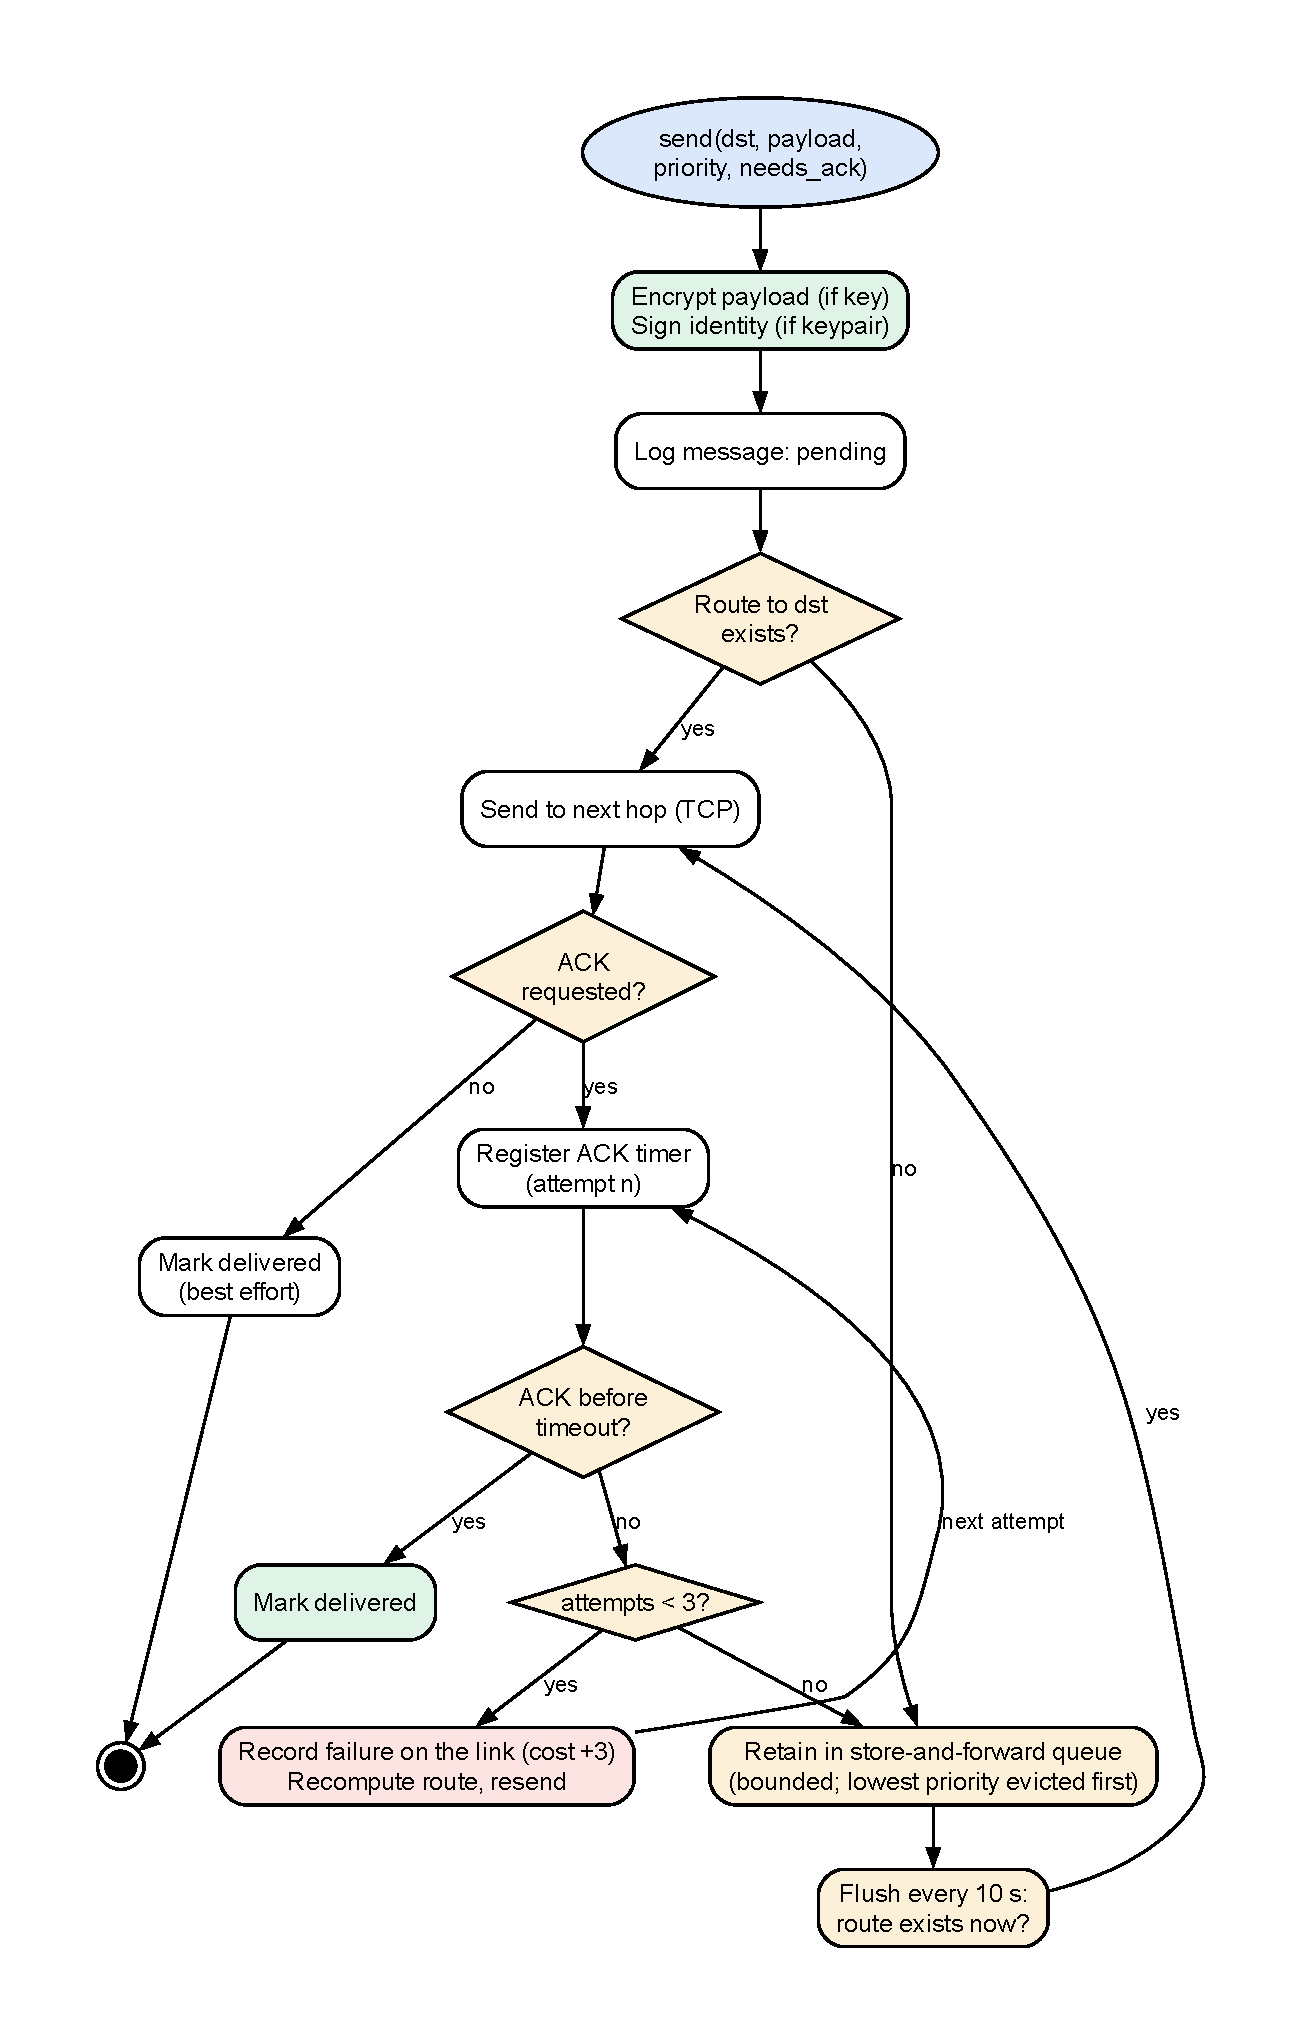
\includegraphics[height=0.36\textheight,keepaspectratio]{figures/fig_flow_send.pdf}
\caption{Flowchart: originate, acknowledge, retry and retain a message}
\label{fig:flowsend}
\end{figure}
\begin{figure}[!htbp]
\centering
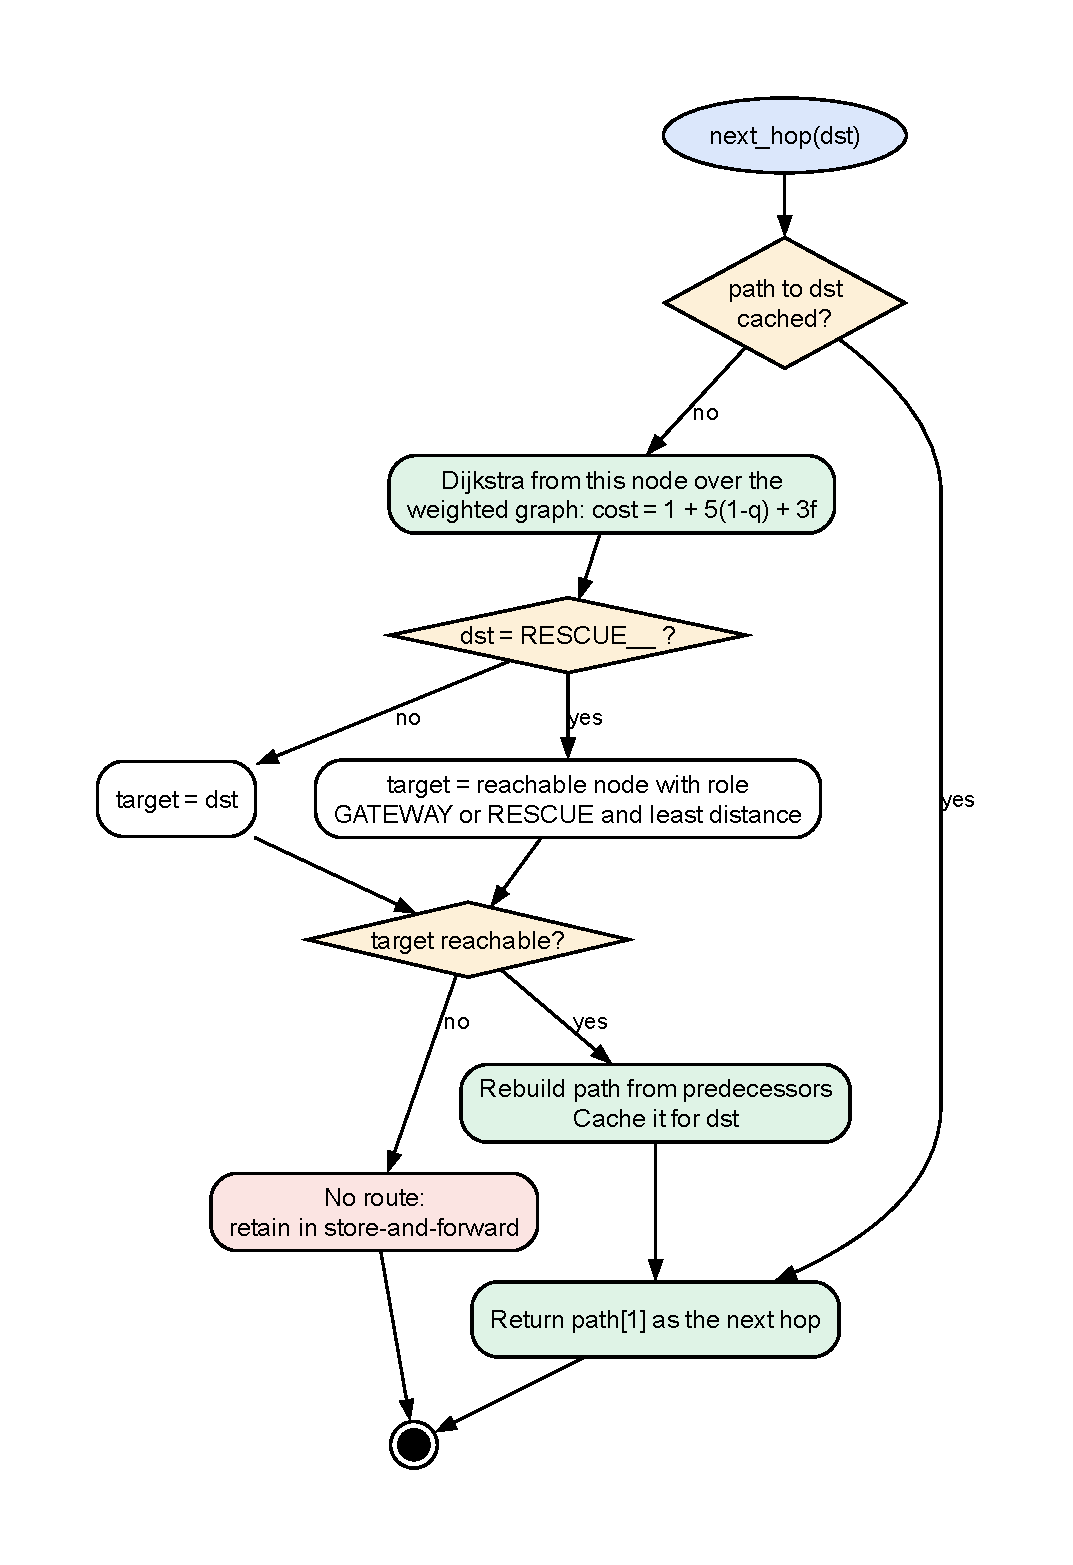
\includegraphics[height=0.32\textheight,keepaspectratio]{figures/fig_flow_route.pdf}
\caption{Flowchart: next-hop selection, including \texttt{RESCUE\_\_}}
\label{fig:flowroute}
\end{figure}

\subsection{Data Structure Selection}
\begin{table}[!htbp]
\caption{Data structures and why they were chosen}
\label{tab:ds}
\footnotesize
\begin{tabularx}{\textwidth}{@{}>{\raggedright\arraybackslash}p{4.2cm}>{\raggedright\arraybackslash}X@{}}
\toprule
\textbf{Structure and use} & \textbf{Reason}\\ \midrule
Adjacency dictionary of dictionaries: \texttt{MeshGraph} & $O(1)$ edge update and lookup, $O(\deg)$ iteration in Dijkstra; the mesh is sparse, so no matrix\\
Binary min-heap: Dijkstra frontier and the message priority queue & $O(\log n)$ insert and extract-min; ordering by (priority, timestamp, counter)\\
Hash map with timestamps: dedup set, neighbour table, route cache & $O(1)$ average membership; expiry by pruning\\
Fixed-capacity deque (20 slots) per neighbour & bounded sliding window for the link-quality estimate\\
Dictionary keyed by message id: ACK tracker, retention queue & $O(1)$ acknowledge and removal\\
Set: visited nodes in Dijkstra, reachable set & $O(1)$ membership\\
\bottomrule
\end{tabularx}
\end{table}

\subsection{Algorithm Selection and Justification}
Flooding delivers, but its message count grows with the square of the node count and it collapses a mesh under load. Bellman--Ford tolerates negative weights, which never occur here, at $O(VE)$; A* needs a geometric heuristic that a building mesh lacks. Dijkstra with a binary heap is correct for non-negative weights and runs in $O((V+E)\log V)$. Hop count, the default metric of the surveyed protocols, picks lossy shortcuts (Chapter~\ref{ch:perf} measures the difference). A sorted list would make insertion $O(n)$ and a FIFO cannot express priority; a hash set gives $O(1)$ duplicate checks where a list gives $O(n)$ on the hot path. The route cache is cleared on any topology change, which is simple and always correct.

\subsection{Time Complexity Analysis}
\begin{table}[!htbp]
\caption{Time complexity ($V$ nodes, $E$ links, $n$ queued packets, $q$ retained messages, $D$ distinct destinations, $|N|$ neighbours)}
\label{tab:complexity}
\footnotesize
\begin{tabularx}{\textwidth}{@{}>{\raggedright\arraybackslash}p{5.8cm}>{\raggedright\arraybackslash}X@{}}
\toprule
\textbf{Operation} & \textbf{Time}\\ \midrule
Dijkstra with the weighted cost & $O((V+E)\log V)$ in every case\\
Link-state merge on receiving a report & $O(\deg(v))$ plus $O(|N|)$ to re-flood\\
HELLO handling & $O(1)$ amortised\\
Priority enqueue / dequeue & $O(\log n)$; draining $n$ packets $O(n\log n)$\\
Duplicate detection & $O(1)$ average\\
Loop check & $O(|\text{path}|)$, at most 10 here\\
Store-and-forward flush & $O(D\,(V+E)\log V+q)$ with the route cache; worst case $O(q\,(V+E)\log V)$\\
Eviction & $O(q)$ scan, only when over the bound\\
Packet parse and validate & $O(1)$ for the fixed 52-byte header\\
\bottomrule
\end{tabularx}
\end{table}
Dijkstra's bound holds for every input. The cache makes repeated lookups to a destination $O(1)$ until a topology change clears it.

\subsection{Space Complexity Analysis}
Per node the graph needs $O(V+E)$ (a few hundred entries at 50 nodes), the dedup set is proportional to the traffic in the 300\,s window, the retention queue is bounded at 500 packets, and the neighbour windows hold $|N|\times 20$ timestamps. Dijkstra needs $O(V)$ extra for distances, predecessors and the heap. The SQLite log grows with the number of events and is the only unbounded structure; it lives on disk, not in memory.

\subsection{Optimization Opportunities}
\label{sec:opt}
Per-destination route-cache invalidation and incremental shortest paths instead of clearing the whole cache; multipoint relays to cut redundant copies of a report~\cite{rfc3626olsr}; short retention at relays (a relay with no route now drops the packet); batched SQLite commits (each event commits, which is safe but limits the logging rate); and the timer changes that the measurements point to (Chapter~\ref{ch:perf}).

\section{Subject-Wise Engineering Concepts and APNI Leap Alignment}
\label{ch:subjects}

\subsection{Concepts Applied, Subject by Subject}
\textbf{Software Engineering.} Seven layers live in separate modules joined only in \texttt{node.py}; the message lifecycle is an explicit state machine (Figure~\ref{fig:state}); every requirement has an identifier and acceptance tests (Table~\ref{tab:frsum}); bad input is dropped and logged, never raised; Git with phase branches and Conventional Commits (Section~\ref{sec:git}).
\textbf{Computer Networks.} Each node is both host and router. The custom binary protocol has a magic value, version and self-describing length, so a stream is framed without a prefix (Table~\ref{tab:header}); HELLO is a one-hop broadcast and DATA and ACK use TCP per hop with the previous hop's identity and 1.5\,s connect bounds. Errors are recovered by TCP, by ACK, retry and re-routing, and by store-and-forward. A central server is deliberately absent; each peer is a server to its neighbours and a client of them.
\textbf{DBMS.} Schema, keys, a deliberately denormalised \texttt{path}, two indexes, upserts and WAL (Section~\ref{sec:db}); every write commits at once; all metrics (delivery ratio, hop histogram, latency percentiles, retries, held and flushed counts) are SQL queries. Each node owns its file, so there is no shared database.
\textbf{Operating Systems.} One process per node; five processes communicate only over TCP and HTTP. A single cooperative \texttt{asyncio} thread needs no locks. Scheduling is \emph{priority scheduling} (SOS, NORMAL, STATUS, oldest first on ties) at every hop; Round-Robin was rejected because an emergency must not share a link fairly. A Windows cancellation race in \texttt{wait\_for} was fixed with a cancellation-safe helper (D5).
\textbf{Data Structures and Algorithms.} Adjacency dictionaries, binary heaps, hash maps and sets, and fixed-size deques (Table~\ref{tab:ds}); Dijkstra is correct because every edge weight is at least 1 and runs in $O((V+E)\log V)$; the cost coefficients are derived (Section~\ref{sec:cost}) and tested against hop count (Chapter~\ref{ch:perf}).
\textbf{Cloud Computing.} Not applicable by design: there is no server, hosted database or autoscaling, and no recurring cost.

\subsection{Mapping of Subjects to Project Implementation}
Table~\ref{tab:subjmap} maps each subject to the concept applied, its module and the evidence.
\begin{table}[!htbp]
\caption{Subjects, concepts applied, modules and evidence}
\label{tab:subjmap}
\footnotesize
\begin{tabularx}{\textwidth}{@{}>{\raggedright\arraybackslash}p{2.6cm}>{\raggedright\arraybackslash}X>{\raggedright\arraybackslash}p{3.4cm}>{\raggedright\arraybackslash}p{3.5cm}@{}}
\toprule
\textbf{Subject} & \textbf{Concept applied} & \textbf{Project module} & \textbf{Evidence}\\ \midrule
Software Engineering & modularity, state machine, error policy, traceability, version control & all; \texttt{node.py} & Table~\ref{tab:frsum}; Section~\ref{sec:git}\\
Computer Networks & binary protocol, framing, per-hop TCP, timeouts, failure detection & \texttt{packet.py}, \texttt{lan\_transport.py} & \texttt{test\_packet}, \texttt{test\_lan\_transport}\\
DBMS & schema, keys, indexes, upserts, WAL, query metrics & \texttt{store.py}, \texttt{api/metrics.py} & \texttt{test\_store}; Section~\ref{sec:db}\\
Operating Systems & process per node, event loop, priority scheduling, bounded memory & \texttt{node.py}, \texttt{reliability.py} & concurrency tests; priority scenario\\
Data Structures & heap, hash map and set, adjacency dictionary, deque & \texttt{routing.py}, \texttt{reliability.py} & \texttt{test\_reliability}, \texttt{test\_dijkstra}\\
Algorithms, Graphs & Dijkstra, cost derivation, link-state flooding & \texttt{routing.py} & weighted vs hop count\\
Cloud Computing & not applicable (no server by design) & -- & --\\
\bottomrule
\end{tabularx}
\end{table}

\section{Implementation and Module-Wise Coding}
\label{ch:impl}

\subsection{Development Environment}
The system is written in Python~3.10 with \texttt{asyncio}, the \texttt{cryptography} library and SQLite; the API uses FastAPI, uvicorn and pydantic; the web application uses React~18, Vite and Tailwind; testing uses pytest and pytest-asyncio; version control is Git on GitHub. The source is about 6\,500 lines of Python (\texttt{mesh/}, \texttt{api/}, \texttt{sim/}, \texttt{story/}), 4\,500 lines of tests and 3\,100 lines of React.

\subsection{Overall Implementation Strategy}
The build order followed what blocks what. \textbf{Phase~1:} the 52-byte packet and the \texttt{Transport} interface, so every track could work against a stable boundary. \textbf{Phase~2:} discovery, single-hop relay and the simulated transport, so that routing and reliability could be tested in one process. \textbf{Phase~3:} routing, reliability, security and storage, wired into \texttt{Node}. \textbf{Phase~4:} the API and React application, the scenario runner and metrics, engine fixes found by integration, and the multi-device deployment.

\subsection{Module-Wise Implementation}
\label{sec:modules}
Table~\ref{tab:impl} gives, for each module, its code reference (file and size), its purpose, input and output, processing logic, dependencies and test evidence.
\begin{table}[!htbp]
\caption{Modules: code reference, logic, dependencies and tests}
\label{tab:impl}
\footnotesize
\begin{tabularx}{\textwidth}{@{}>{\raggedright\arraybackslash}p{3.55cm}>{\raggedright\arraybackslash}X>{\raggedright\arraybackslash}p{2.25cm}>{\raggedright\arraybackslash}p{1.8cm}@{}}
\toprule
\textbf{Module (lines)} & \textbf{Purpose, input $\rightarrow$ output, processing, details} & \textbf{Depends on} & \textbf{Tests}\\ \midrule
\texttt{mesh/core/packet.py} (362) & wire format, \texttt{Packet} $\leftrightarrow$ bytes. \texttt{struct} format asserted to be 52 bytes; every field range-checked; \texttt{unpack} rejects bad magic and truncation of each region; \texttt{remaining\_length} frames stream reads; \texttt{identity\_bytes} is the signed content & -- & 47 + 4\,000 fuzz\\
transports (461) & bytes between neighbours: simulated (seeded loss, latency), multicast/TCP, and the multi-device \texttt{LanTransport} (Section~\ref{sec:lan}) & \texttt{packet} & 15 + 6\\
\texttt{discovery.py} (292) & HELLOs $\rightarrow$ neighbour table, peer events, link quality over a 20-slot window reported only when it moves by 0.1; \texttt{visible\_neighbours} range emulation & \texttt{transport} & 15 + 12\\
\texttt{relay.py} (153) & received packets $\rightarrow$ deliver, forward or drop (algorithm A4); one drain task over a priority queue & \texttt{reliability} & 18 + 3\\
\texttt{routing.py} (546) & reports $\rightarrow$ graph, next hop. \texttt{MeshGraph}, \texttt{edge\_cost}, sequence-numbered gossip with quality, failures, role and key, cached Dijkstra, \texttt{RESCUE\_\_} terminals, hop-count switch for the comparison & \texttt{discovery} & 14 + 14 + 33\\
\texttt{reliability.py} (240) & \texttt{DedupSet} (300\,s), \texttt{MessagePriorityQueue}, \texttt{AckTracker} (3 attempts), \texttt{StoreForwardQueue} (500 messages, 1800\,s) & \texttt{packet} & 18 + 20\\
\texttt{crypto.py} (131) & AES-256-GCM with nonce prefix and associated data; Ed25519 sign and non-raising verify; one exception type & \texttt{cryptography} & 19\\
\texttt{store.py} (258) & tables, WAL, upserts, event queries, \texttt{events\_since}, listing and counting for metrics & \texttt{sqlite3} & 23\\
\texttt{node.py} (513) & composition root: \texttt{send()} encrypts, signs, logs, dispatches; receive verifies, decrypts, logs, ACKs; ACK loop records the failure, recomputes, resends; flush loop expires and retries & all above & 27\\
\texttt{sim/}, \texttt{api/lab.py}, \texttt{api/metrics.py} (3\,000) & simulator with a virtual clock and seven scenarios; metrics read from node logs & \texttt{node} & 5 + 12\\
\bottomrule
\end{tabularx}
\end{table}

\subsection{Front-End Implementation}
The front end is one app: the \textbf{device screen} (\texttt{story/node.html}), a single page served by every device that becomes a \emph{survivor phone}, a \emph{gateway} view or a \emph{rescue console} according to the device's role. A phone is only a screen: the engine runs on the laptop and the phone opens the page over the same Wi-Fi or hotspot. The survivor screen is built to be read under stress: a plain status line, need buttons (need help, trapped, injured, fire or smoke, water or food), a location field, an SOS button held about 1.2\,s to prevent accidental sends, an ``I am safe'' check-in that never delays an SOS, a form to send a text message to a named device, the rescue team's reply shown above a plain-language progress tracker, and the nearby phones with signal strength. The rescue console shows each request with its need, location, route and age; a separate Marked safe list; filters by type and need; a reply action with quick replies; message history with priority and direction filters; CSV export of the received requests; counters; and a network map that shows link quality and highlights the route of a new message. Every screen also has a live panel, ``What this device is doing'', that words the device's own event log in plain English, so discovery and routing can be watched happening. Screens are shown in Section~\ref{sec:shots}. The \textbf{simulation lab} (\texttt{ui/}, a React PWA served by \texttt{api/server.py}) is no longer part of the demonstration. It stays in the repository because it produced the experiments: it runs many real nodes over the simulated radio, switches nodes off and on, edits links, and offers pages for routing, reliability, the wire protocol, security and the simulator.

\subsection{Back-End Implementation}
The back end is FastAPI with a WebSocket. The engine server (\texttt{api/server.py}) exposes the simulation lab (snapshot, reset, kill and revive, link edits, bursts), a node's view, graph and route (weighted and hop-count), \texttt{send} and \texttt{sos}, the rescue view, statistics, one message's full story, the event log, a protocol inspector, a security playground and attack drill, background scenario jobs, and \texttt{/ws}, which streams every logged event. Each device server (\texttt{story/node.py}) exposes \texttt{/api/me} (everything its screen needs), \texttt{/api/sos} (the need and location travel as structured fields), \texttt{/api/send} (a text message to a named device), \texttt{/api/safe} (an ``I am safe'' check-in at the lowest priority), \texttt{/api/events} (the event log in plain English), \texttt{/api/history} (messages filtered by priority and direction), \texttt{/api/export.csv} (the received requests, rescue device only) and \texttt{/api/power}; started with \texttt{--phone} it serves its screen on every network interface so a phone on the same Wi-Fi can open it. Request bodies are validated with pydantic, and engine errors map to clear HTTP errors.

\subsection{Database Implementation}
The three tables of Section~\ref{sec:db} are created with \texttt{CREATE TABLE IF NOT EXISTS}, WAL mode is set at connection time, and the two indexes are created with the schema. Queries used include retained messages by status (\texttt{SELECT * FROM messages WHERE status = ?}), a message's timeline (\texttt{SELECT * FROM events WHERE msg\_id = ? ORDER BY ts\_ms}), event counters (\texttt{SELECT COUNT(*) FROM events WHERE kind = ?}), and the upsert \texttt{INSERT \ldots ON CONFLICT(msg\_id) DO UPDATE}. Every write commits immediately.

\subsection{Communication and Concurrency Implementation}
\label{sec:lan}
The original \texttt{UdpTcpTransport} could not carry a complete \texttt{Node}: it never learned a HELLO sender's address, and it reported the packet's \emph{original} source instead of the previous hop, which breaks link-state flooding. \texttt{lan\_transport.py} fixes both. A JSON \textbf{topology file} lists every device (role, host, port) and the links (who can hear whom); a device talks only to its configured neighbours, which is the range emulation of the honest statement and satisfies DIS-7, so no multicast is needed. Each connection starts with the previous hop's identity followed by the unmodified packet. A \textbf{power switch} makes a device neither send nor hear, like a dead radio. \texttt{python -m story.node --id L1} starts one device (engine plus a small web server); five of them, started together on one machine or one per laptop, form the mesh, each with its own SQLite log, port and screen. In the two-laptop demonstration L1--L3 ran on one laptop and L4--L5 on the other, joined through a phone hotspot (Figure~\ref{fig:deploy}). Recovery is layered: TCP per hop; ACK, retry and re-route end to end; store-and-forward when retries run out.

\subsection{Git Repository Setup}
\label{sec:git}
\textbf{Repository:} \url{\RepoURL}. \textbf{Structure:} \texttt{mesh/core/} (engine), \texttt{api/}, \texttt{sim/}, \texttt{story/}, \texttt{ui/}, \texttt{tests/}, \texttt{docs/}, \texttt{config/}, with README, CONTRIBUTING and requirements from the first phase. \textbf{Branching strategy:} one branch per phase, each inheriting the previous and never merged back (\texttt{develop}, \texttt{develop\_2}, \texttt{develop\_3}, \texttt{develop\_4}, \texttt{develop\_5}). \textbf{Commit conventions:} Conventional Commits (\texttt{feat(routing): \ldots}, \texttt{fix(reliability): \ldots}). \textbf{Contribution of members:} Miti Shah built discovery, the relay, the node skeleton and the simulated transport in Phase~2 and, in Phase~3, Dijkstra pathfinding with gateway and rescue handling and route caching, the dedup set and priority queue, ACK tracking with retry and the store-and-forward queue, AES-256-GCM encryption with Ed25519 signing, and the SQLite log; Twissha Shah built the weighted cost function and link-state gossip, the wiring of routing, reliability, crypto and storage into the node, the multi-device program and device screens, the robustness and socket tests, and the evidence scripts; Tanvi Sheth built the packet format, transports, the API, the React application and the scenario runner, and the Phase~4 engine fixes found by integration. Nine of Miti's Phase~3 commits were made from Twissha's laptop and were first recorded under Twissha's Git account; they were re-attributed to Miti on 24 October 2026 with the agreement of all three members, and the correction is recorded in \texttt{docs/contribution-log.md}. \textbf{Evidence of development history:} Table~\ref{tab:commits}.

\begin{table}[H]
\caption{Commits per team member, read from \texttt{git log --all} (45 commits)}
\label{tab:commits}
\small
\begin{tabular}{@{}lrr@{}}
\toprule
\textbf{Member} & \textbf{Commits} & \textbf{Share}\\ \midrule
Twissha Shah & 24 & 53\,\%\\
Tanvi Sheth & 19 & 42\,\%\\
Miti Shah & 2 & 4\,\%\\
\bottomrule
\end{tabular}
\end{table}
\textbf{Conventional Commits.} 40 of 45 commits (89\,\%) follow the \texttt{type(scope): subject} convention of \texttt{CONTRIBUTING.md}.

\textbf{Branches:} \texttt{main}, \texttt{develop}, \texttt{develop\_2}, \texttt{develop\_3}, \texttt{develop\_4}. \textbf{Tags:} \texttt{v0.3-phase3}.


\subsection{Integration of Modules}
\texttt{Node} registers one dispatcher on the transport that feeds each packet to discovery (HELLO), gossip (LINK\_STATE) and relay (DATA, ACK); each ignores types it does not own. Callbacks connect the pieces: peer-up sets a one-hop route and a graph edge and logs the event; a topology change invalidates cached routes; relay hooks write the message and event log; the ACK loop reports failures to gossip so the cost reacts at once. The API reads the same objects and database, so nothing on screen is computed separately from the engine.

\subsection{Implementation Challenges and Resolutions}
The significant difficulties (Table~\ref{tab:defects} gives each cause and retest) were: a single receive callback that let only one of discovery and relay hear packets; topology known only two hops out, with dead nodes still routable; signatures that failed after the first relay (fixed by signing identity fields only); ACKs and retries lost at relays; a hostile packet raising \texttt{UnicodeDecodeError}; a hang in \texttt{Node.stop()} on Windows; and a transport that could not run a full node (fixed by \texttt{LanTransport}).

\section{Scalability, Performance and Resource Management}
\label{ch:perf}
\providecommand{\CollN}{50}\providecommand{\CollDel}{92.6}\providecommand{\CollDelMin}{76}\providecommand{\CollDelMax}{100}\providecommand{\CollRecMean}{8.1}\providecommand{\CollRecMax}{10.25}\providecommand{\CollRecN}{50}\providecommand{\CollRecOK}{23}\providecommand{\CollConvMean}{9.6}\providecommand{\CollConvMax}{15.2}

\providecommand{\HopW}{99.2}\providecommand{\HopH}{57.4}\providecommand{\HopWins}{20}\providecommand{\HopRuns}{20}

\providecommand{\SosAdv}{4.4}

\providecommand{\ThrMaxN}{2000}\providecommand{\ThrMaxRate}{4686}\providecommand{\ThrMidRate}{7029}\providecommand{\ThrMaxAck}{1.0}


Every number here is generated from stored measurements by \texttt{docs/report/evidence/}. The \emph{simulator} (real nodes over an in-memory transport with seeded loss on a virtual clock) and \emph{live devices} (real processes, TCP and timers) are never mixed.

\subsection{Scalability Requirements}
The SRS requires 50 nodes, 90\,\% delivery on 40 nodes at 20\,\% loss, convergence within 15\,s and recovery within 10\,s (Section~\ref{sec:kpi}); sizes above five exist only in the simulator.
\subsection{Workload and Load Model}
Each scenario fixes a topology, per-link loss, 5--40\,ms latency, 10--90 messages and a failure script, repeated over seeds so routing modes see identical traffic. Sweeps vary loss 0--50\,\% (21 nodes) and size 10--65 nodes; throughput uses 100--2\,000 sends; the live run sent 30 SOS with 8 relay failures and 4 gateway outages.

\subsection{Resource Utilization}
\textbf{Simulator:} 65 nodes used about 13\,MB of heap (Table~\ref{tab:scale}). \textbf{Live:} about 55\,MB and 0.2--1.0\,\% of a core per idle process (Table~\ref{tab:live}). \textbf{Storage:} one log row per event; at most 500 held messages. \textbf{Network:} transmissions per delivery in Table~\ref{tab:scale}.
\subsection{Concurrent Processing}
A node is single-threaded and cooperative with no locks. On a three-node line with ACKs, \ThrMidRate\ messages per second were delivered at 1\,000 simultaneous sends and \ThrMaxRate\ per second at \ThrMaxN\ (all ACKed within \ThrMaxAck\,s); the concurrency tests (Chapter~\ref{ch:test}) confirm exactly-once delivery.

\subsection{Scheduling and Synchronization Analysis}
Scheduling is by priority, oldest first on ties, at every hop; its metric is the SOS latency advantage under congestion (Section~\ref{sec:perfresults}), since an idle network has nothing to overtake. No synchronisation primitive is needed: shared state lives on the event-loop thread.

\subsection{Performance Measurement}
One Windows~11 laptop, Python~3.10; live runs used five loopback processes with shortened timers. Memory and CPU come from OS counters, live latency from polling every 20\,ms, and simulator metrics from SQL over the node logs.
\subsection{Performance Results}
\label{sec:perfresults}
\textbf{Reliability under loss} (Figure~\ref{fig:results}a, 21-node grid, 8 seeded runs per point). Delivery stays at or above 98\,\% to 20\,\% loss and falls to 61\,\% at 50\,\%; each lost ACK costs a 4\,s timeout, so median latency goes from tens of milliseconds at 0\,\% to seconds at 20--30\,\%.

\textbf{Scenarios.}
\begin{table}[htbp]
\caption[Results of the seven simulator scenarios]{Results of the seven simulator scenarios (weighted routing; delivery ratio shown as mean (min--max) over the runs)}
\label{tab:scenarios}
\footnotesize
\setlength{\tabcolsep}{4pt}
\begin{tabular}{@{}>{\raggedright\arraybackslash}p{0.148\textwidth}>{\raggedleft\arraybackslash}p{0.063\textwidth}>{\raggedleft\arraybackslash}p{0.057\textwidth}>{\raggedleft\arraybackslash}p{0.057\textwidth}>{\raggedleft\arraybackslash}p{0.194\textwidth}>{\raggedleft\arraybackslash}p{0.051\textwidth}>{\raggedleft\arraybackslash}p{0.068\textwidth}>{\raggedleft\arraybackslash}p{0.068\textwidth}>{\raggedleft\arraybackslash}p{0.137\textwidth}@{}}
\toprule
\textbf{Scenario} & \textbf{Nodes} & \textbf{Loss} & \textbf{Runs} & \textbf{Delivery} & \textbf{Hops} & \textbf{Conv. (s)} & \textbf{Recov. (s)} & \textbf{S\&F flushed / queued} \\ \midrule
baseline\_\allowbreak{}10 & 10 & 5\% & 20 & 100.0\,\% (100--100) & 1 & 5.5 & -- & 7/7 \\
collapse\_\allowbreak{}40 & 40 & 20\% & 50 & 92.6\,\% (79--100) & 4 & 9.6 & 8.1 & 2919/3117 \\
no\_\allowbreak{}gateway & 12 & 5\% & 20 & 100.0\,\% (100--100) & 2 & 5.2 & -- & 207/207 \\
high\_\allowbreak{}loss & 20 & 35\% & 20 & 89.3\,\% (74--100) & 2 & 17.7 & -- & 1045/1076 \\
chain\_\allowbreak{}10hop & 11 & 5\% & 20 & 100.0\,\% (100--100) & 9 & 14.4 & -- & 87/90 \\
hopcount\_\allowbreak{}vs\_\allowbreak{}weighted & 5 & 45\% & 20 & 99.2\,\% (90--100) & 2 & 5.2 & -- & -- \\
priority\_\allowbreak{}load & 16 & 0\% & 20 & 100.0\,\% (100--100) & 2 & 7.6 & -- & 1356/1356 \\
\bottomrule
\end{tabular}
\par\smallskip\footnotesize Hops = median hop count of delivered messages. Conv. = mean seconds until every node's graph contains every node. Recov. = mean seconds from relay death until the sender has a route avoiding it. S\&F counts are event counts summed over all runs: a message re-queued after a failed retry is counted each time, and messages still held when a run ends are not flushed.
\end{table}

The 40-node collapse scenario (20\,\% loss, a relay on the active path killed at $t=10$\,s, the gateway killed at 25\,s and revived at 60\,s) delivered \CollDel\,\% on average over \CollN\ seeded runs (worst \CollDelMin\,\%, best \CollDelMax\,\%). At 35\,\% loss (outside the specified condition) delivery was 89.1\,\%.
\begin{figure}[!tb]
\centering
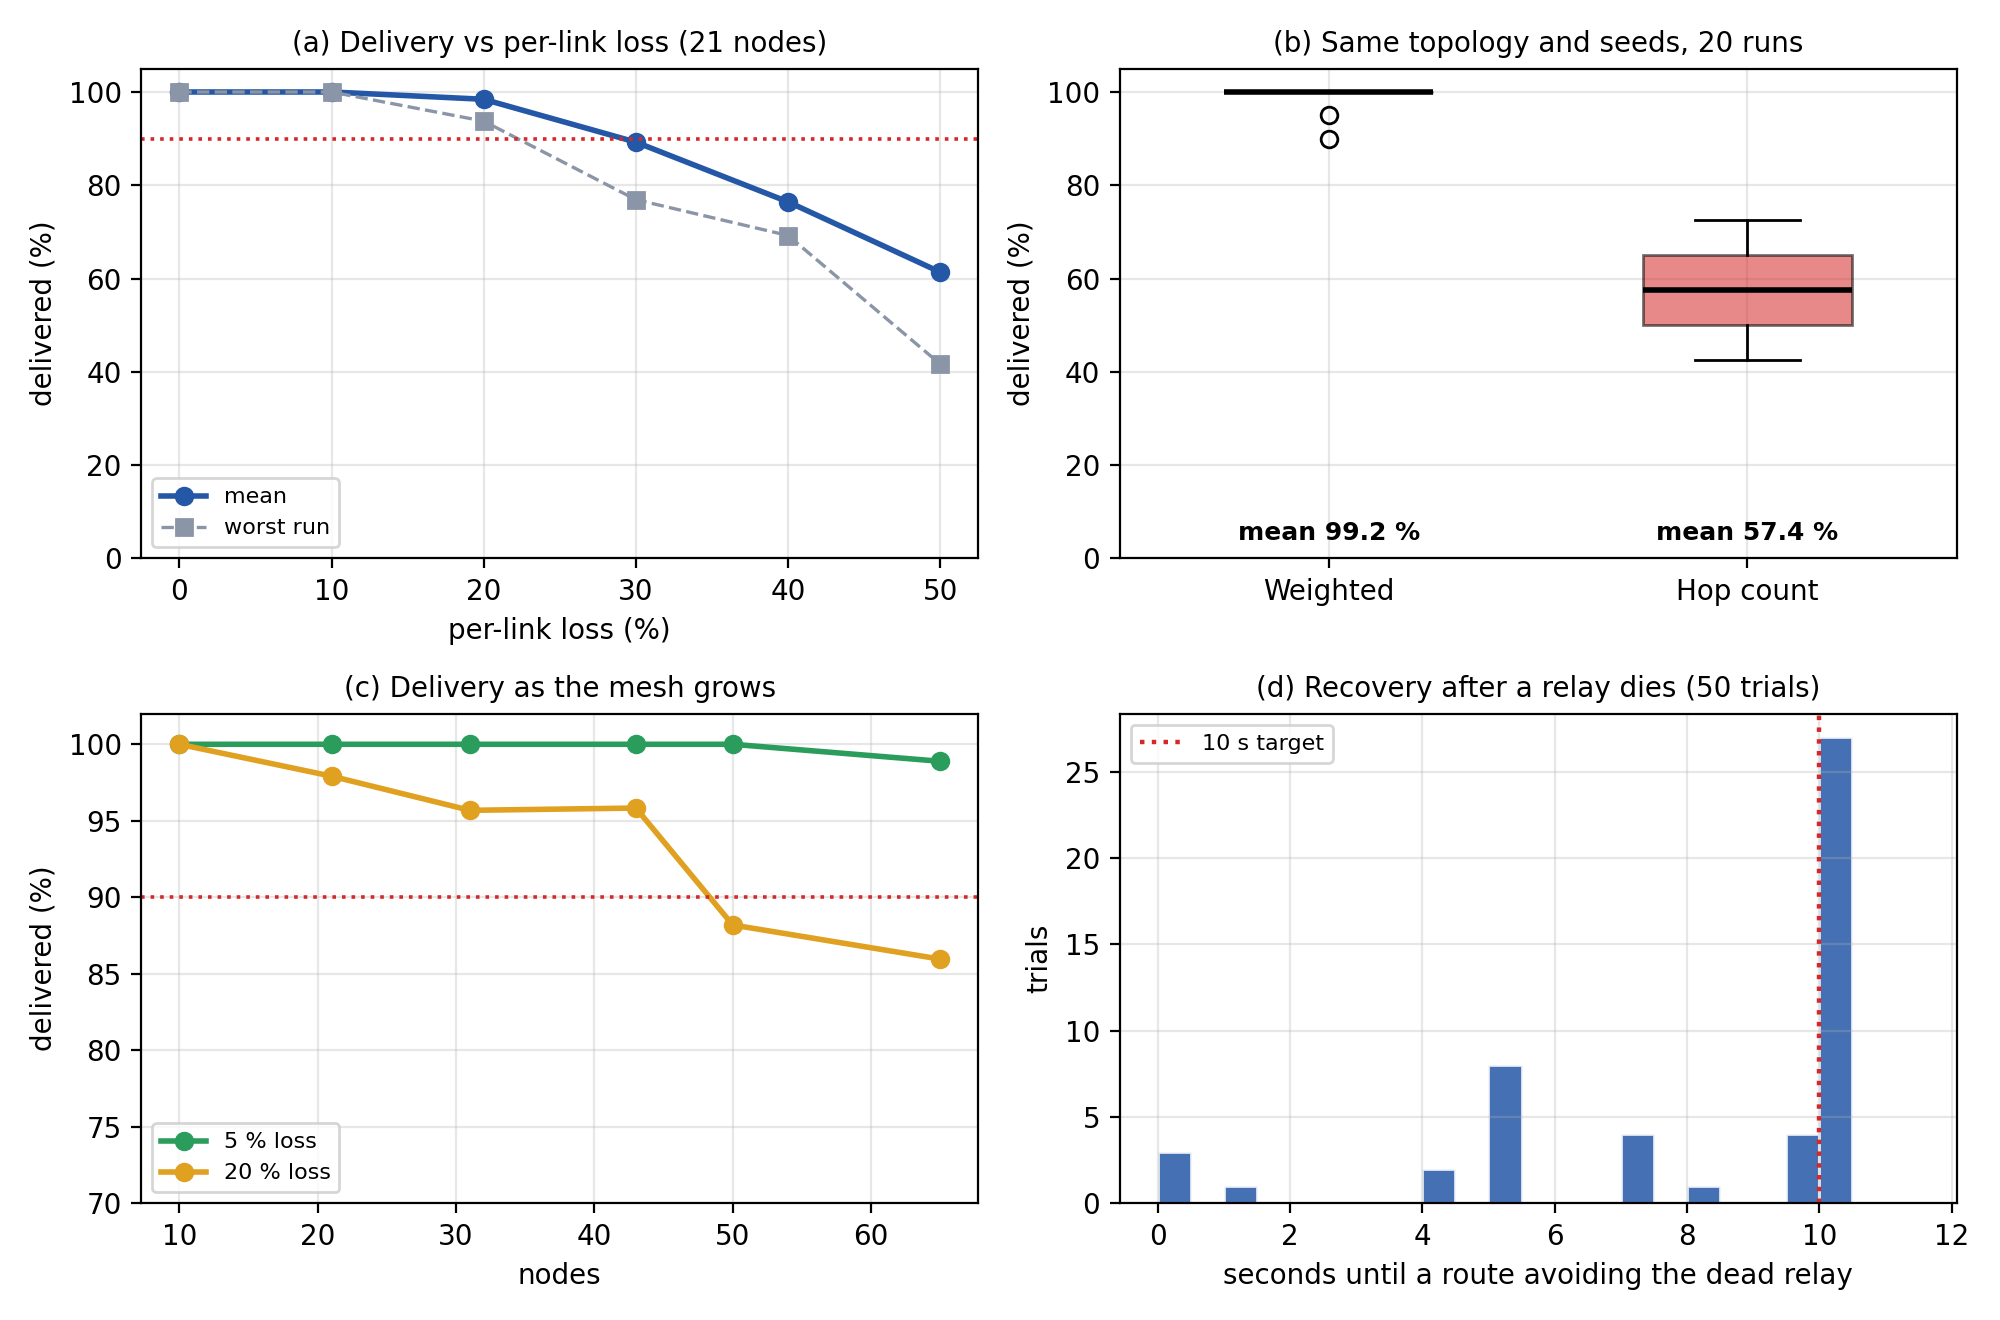
\includegraphics[width=0.86\textwidth]{figures/fig_results.png}
\caption[Delivery, routing comparison, scale and recovery results]{(a) Delivery against per-link loss. (b) Weighted versus hop-count routing on identical seeds. (c) Delivery as the mesh grows. (d) Recovery time after a relay death, 50 trials.}
\label{fig:results}
\end{figure}
\textbf{Weighted versus hop-count routing (Figure~\ref{fig:results}b).} A 2-hop shortcut crosses a link with 45\,\% loss while a 3-hop path is clean, and messages are best-effort, so a poor route shows directly as loss. Weighted routing delivered \HopW\,\% and hop count \HopH\,\%, weighted winning on \HopWins\ of \HopRuns\ identical seeds. The topology is \emph{designed} to expose hop count, so it shows that the cost avoids a lossy shortcut, not that every mesh has this gap.

\textbf{Priority under load.} The congested scenario (16 nodes, 90 messages to the same destination, 15\,\% SOS) gives an SOS a median latency \SosAdv$\times$ lower than routine traffic. Only here do both take the same trip, so the comparison is fair.

\textbf{Scalability.}
\begin{table}[htbp]
\caption[Scalability, 10 to 65 simulated nodes]{Scalability, 10 to 65 simulated nodes (10 runs per size and loss rate)}
\label{tab:scale}
\footnotesize
\setlength{\tabcolsep}{4pt}
\begin{tabular}{@{}>{\raggedleft\arraybackslash}p{0.077\textwidth}>{\raggedleft\arraybackslash}p{0.077\textwidth}>{\raggedleft\arraybackslash}p{0.100\textwidth}>{\raggedleft\arraybackslash}p{0.100\textwidth}>{\raggedleft\arraybackslash}p{0.100\textwidth}>{\raggedleft\arraybackslash}p{0.100\textwidth}>{\raggedleft\arraybackslash}p{0.115\textwidth}>{\raggedleft\arraybackslash}p{0.084\textwidth}>{\raggedleft\arraybackslash}p{0.092\textwidth}@{}}
\toprule
\textbf{Nodes} & \textbf{Links} & \textbf{Delivery at 5\% loss} & \textbf{Delivery at 20\% loss} & \textbf{Tx per delivered (5\%)} & \textbf{Tx per delivered (20\%)} & \textbf{Conv. max at 20\% (s)} & \textbf{CPU (s, 5\%)} & \textbf{Heap (MB, 5\%)} \\ \midrule
10 & 13 & 100.0\,\% & 100.0\,\% & 5.0 & 8.9 & 15.2 & 3 & 0.7 \\
21 & 32 & 100.0\,\% & 98.8\,\% & 7.4 & 16.1 & 15.2 & 13 & 1.7 \\
31 & 50 & 100.0\,\% & 96.2\,\% & 10.6 & 26.5 & 15.2 & 43 & 3.0 \\
43 & 72 & 100.0\,\% & 96.2\,\% & 12.2 & 24.8 & 20.2 & 91 & 5.3 \\
50 & 85 & 100.0\,\% & 92.9\,\% & 14.2 & 31.9 & 15.2 & 110 & 6.5 \\
65 & 113 & 98.0\,\% & 83.1\,\% & 20.6 & 39.4 & 15.2 & 188 & 9.8 \\
\bottomrule
\end{tabular}
\par\smallskip\footnotesize Nodes and links include the gateway and rescue post added to the grid. Tx = hop-by-hop data transmissions. CPU and heap are for the whole simulated mesh in one process on a virtual clock, not the cost of one real device.
\end{table}

At 5\,\% loss delivery is 100\,\% to 50 nodes and 98.0\,\% at 65; at 20\,\% loss it is 92.9\,\% at 50 and 83.1\,\% at 65. Transmissions per delivery grow about linearly with size, not quadratically as with flooding.

\textbf{Recovery and convergence} follow the timers (Figure~\ref{fig:results}d): convergence comes in multiples of the 5\,s gossip interval, and recovery took under 10\,s in 24 of 50 trials and 10.2--10.25\,s in the rest, bounded by the 10\,s heartbeat timeout.

\textbf{Live devices.} Table~\ref{tab:live} gives five real processes over real TCP.
\begin{table}[H]
\caption{Live devices: 5 operating-system processes, real TCP sockets, real timers, on one laptop (loopback)}
\label{tab:live}
\footnotesize
\setlength{\tabcolsep}{4pt}
\begin{tabular}{@{}>{\raggedright\arraybackslash}p{0.482\textwidth}>{\raggedright\arraybackslash}p{0.482\textwidth}@{}}
\toprule
\textbf{Measurement} & \textbf{Result} \\ \midrule
Process start \textrightarrow{} every device knows every device & 3.8 s \\
SOS arrives at the rescue device (30/30 delivered) & median 47 ms, 95th pct 102 ms, max 281 ms \\
ACK back at the sender & median 63 ms, 95th pct 149 ms \\
Relay switched off \textrightarrow{} sender re-routes (8 trials) & median 4.0 s, max 4.5 s; every later SOS delivered \\
Gateway down, 5 SOS held; gateway back (4 trials) & 100\% flushed, median 4.5 s, max 6.1 s \\
Device API response (200 requests) & median 16 ms, 95th pct 31 ms \\
Per-process memory and CPU, idle & 53--54 MB; 0.4--1.9\% of one core \\
Per-process CPU while sending SOS (includes the harness polling every 20 ms) & up to 19\% of one core \\
\bottomrule
\end{tabular}
\par\smallskip\footnotesize Timer settings: HELLO 1 s, neighbour timeout 4 s, link-state 2 s, ACK timeout 3 s. Latency is measured by polling each device's own API every 20 ms (up to 20 ms of error). Wireless delay and loss are not included.
\end{table}


\subsection{Bottleneck Identification}
The 10\,s heartbeat timeout (which bounds recovery), the 4\,s ACK timeout under loss, the 5\,s link-state interval, one SQLite commit per event and whole-cache route invalidation.
\subsection{Optimization and Improvement}
No optimisation followed these measurements, so there is no before-and-after comparison; the data point to a shorter, adaptive neighbour timeout, an immediate link-state report on change, an adaptive ACK timeout and per-destination invalidation.
\subsection{Cloud Deployment and Resource Utilization}
Not applicable: there is no server and no cloud deployment.
\subsection{Scalability Limitations}
Tested to 65 simulated nodes and 5 live devices; larger meshes, wireless interference and mobility were not tested.

\section{Testing and Validation}
\label{ch:test}
\providecommand{\NTests}{334}\providecommand{\NRuns}{3}\providecommand{\NClean}{3}

\providecommand{\NFR}{68}\providecommand{\NAuto}{52}\providecommand{\NAutoUI}{10}\providecommand{\NPartial}{2}\providecommand{\NInspect}{2}\providecommand{\NManual}{2}


\subsection{Testing Strategy}
Testing is layered, and each layer answers a different question: unit (does a module behave in isolation), integration (do modules work together in a node, between nodes, through the API and over real sockets), functional (does each SRS requirement hold), non-functional (reliability, scalability, performance, availability, security, usability), boundary and invalid-input, concurrency and stress, and live-device tests. The key design choice is the simulated transport: routing and reliability run on a deterministic in-memory network, so a failure reproduces from a seed. The suite has \NTests\ automated test cases, run completely \NRuns\ times for the results below.
Complete suite runs: 3; fully green: 2. Inconsistent test(s): \texttt{test\_\allowbreak{}api::test\_\allowbreak{}node\_\allowbreak{}view\_\allowbreak{}reports\_\allowbreak{}peers\_\allowbreak{}with\_\allowbreak{}hop\_\allowbreak{}distance}.


\subsection{Unit Testing}
Unit tests cover each module on its own: the packet format (47 tests: round trips, every field's range, null padding, truncation of each region, bad magic, signable and identity bytes, retransmission counter); the cost function and graph; Dijkstra including caching and \texttt{RESCUE\_\_}; gossip encoding and merging; discovery and link quality; the dedup set, priority queue, ACK tracker and store-and-forward bounds; AES-GCM and Ed25519; the SQLite log; the relay; and the simulated transport.

\subsection{Integration Testing}
\texttt{test\_node} (27 tests) runs discovery and relay on one transport, auto-relaying, role propagation, multi-hop origination via re-flooded reports, ACK, the whole message lifecycle in the database, encryption and signing end to end, retry exhaustion into retention, eviction and expiry. \texttt{test\_ack\_multihop} checks that the ACK returns over the data's path, that a lost ACK is re-sent and that a retry crosses relays that saw the original. \texttt{test\_api} drives front end, back end and engine through FastAPI's test client, including the WebSocket: a converged snapshot, an SOS reaching the rescue queue, node views, kill and revive, the event stream, the protocol inspector and the security drill. \texttt{test\_lan\_transport} checks previous-hop identity, range emulation, the power switch, hostile bytes, a dead peer failing fast, and a full three-node mesh over TCP. The React interface and device screens have no automated browser tests; they were inspected by running them (Section~\ref{sec:shots}).

\subsection{Functional Testing}
\label{sec:func}
Table~\ref{tab:fr} lists every requirement with its acceptance criterion, the tests that must pass. 68 functional requirements: 52 verified by automated tests alone, 10 by automated tests plus a manual check of the screen, 2 partially implemented, 2 by code inspection, 2 by manual check only.
 All mapped tests passed in every complete run except one timing-sensitive test that failed once (Section~\ref{sec:defects}). Two requirements are only partly met and are reported as such: SNF-3 (an immediate delivery attempt when a new neighbour appears; retained messages are instead retried every flush interval) and LOG-5 (the history filter exists in the store but the screens have no filter control).

\subsection{Non-Functional Testing}
\label{sec:nonfunc}
\textbf{Reliability:} delivery at 0--50\,\% injected loss (Table~\ref{tab:loss}). \textbf{Scalability:} 10 to 65 nodes at 5\,\% and 20\,\% loss (Table~\ref{tab:scale}). \textbf{Performance:} latency by priority (Table~\ref{tab:priority}), throughput, and live latency (Table~\ref{tab:live}). \textbf{Availability:} recovery over 50 simulated trials and 8 live failovers (Figure~\ref{fig:results}). \textbf{Security:} a relay without the session key never sees the plaintext (\texttt{test\_relay\_never\_sees\_plaintext\_payload}); a tampered ciphertext or a wrong key is detected and dropped; a forged-signature SOS and an unknown signer are rejected; signatures verify across multi-hop relays; and the API's attack drill checks that every attack is defended. \textbf{Usability:} the SOS control is a single hold of about 1.2\,s on one prominent button with plain-language status; a timed study with participants was not carried out (Section~\ref{sec:limits}).

\subsection{Boundary and Invalid-Input Testing}
\label{sec:boundary}
Tests cover empty and header-only input; a bad magic value; truncated header, path, payload and signature; TTL out of range; a payload over the 16-bit length; a path that is too long; node ids over 8 bytes or not ASCII; a wrong-length signature; the signed flag without a signature; a wrong key size; ciphertext shorter than the nonce; an empty payload (valid); and a send to an unknown destination (held, not an exception). \texttt{test\_robustness} also feeds 3\,000 random byte strings and 1\,000 bit-flipped valid packets to the parser and 200 garbage buffers to a running node, requiring only ``parsed'' or ``rejected with \texttt{PacketError}'' and that the node still delivers a normal message afterwards.

\subsection{Concurrency and Stress Testing}
\label{sec:stress}
200 simultaneous sends over two hops with ACKs: all 200 delivered exactly once and every ACK returned. Two senders sending 50 SOS and 50 routine messages simultaneously to one gateway: all 100 arrive intact. One packet replayed five times: delivered once, four duplicates dropped. Throughput up to 2\,000 simultaneous sends (Section~\ref{sec:perfresults}) and the congested priority scenario complete the stress tests. Because shared state lives on one thread, races and deadlocks cannot occur by construction; the tests confirm exactly-once delivery and stability under load.

\subsection{Test Case Specification}
\label{sec:tcs}
\begin{table}[!htbp]
\caption{Representative test cases (every requirement's tests are in Table~\ref{tab:fr})}
\label{tab:tcs}
\scriptsize
\begin{tabularx}{\textwidth}{@{}>{\raggedright\arraybackslash}p{0.8cm}>{\raggedright\arraybackslash}p{1.1cm}>{\raggedright\arraybackslash}X>{\raggedright\arraybackslash}X>{\raggedright\arraybackslash}X>{\raggedright\arraybackslash}p{0.9cm}@{}}
\toprule
\textbf{ID} & \textbf{Req.} & \textbf{Scenario, input and preconditions} & \textbf{Expected result} & \textbf{Actual result and evidence} & \textbf{Result}\\ \midrule
TC-01 & RTE-3, 4 & short path over a lossy link, long path over clean links & Dijkstra takes the clean path & as expected; \texttt{test\_dijkstra} & Pass\\
TC-02 & RTE-8 & report from a node two hops away & re-flooded; graph complete beyond the neighbour & as expected; \texttt{test\_link\_state} & Pass\\
TC-03 & PRI-3 & SOS reaches a relay with routine packets queued & SOS forwarded first & as expected; \texttt{test\_relay} & Pass\\
TC-04 & REL-5, 6 & ACK lost; sender times out & route recomputed, resent, destination sees it once & as expected; \texttt{test\_ack\_multihop} & Pass\\
TC-05 & SNF-1, 2 & no route; a route later appears & held, then flushed and delivered & as expected; live: 4 of 4 outages flushed (Table~\ref{tab:live}) & Pass\\
TC-06 & SNF-5 & retention queue full & lowest priority evicted; an SOS is never displaced & as expected; \texttt{test\_ack\_retry} & Pass\\
TC-07 & SEC-5 & forged-signature packet & rejected and logged & as expected; \texttt{test\_node} & Pass\\
TC-08 & FWD-6 & 3\,000 random byte strings & only \texttt{PacketError}; node survives & one defect found and fixed (D4); \texttt{test\_robustness} & Pass\\
TC-09 & DIS-7 & three nodes over real TCP, neighbour-restricted & routes learned; message and ACK delivered & as expected; \texttt{test\_lan\_transport} & Pass\\
TC-10 & K1 & 40 nodes, 20\,\% loss, relay and gateway failures, 50 seeds & delivery $\ge$ 90\,\% & \CollDel\,\% (worst run \CollDelMin\,\%); Table~\ref{tab:scenarios} & Pass\\
TC-11 & K3 & kill the relay on the active path, 50 trials & re-route $\le$ 10\,s & mean \CollRecMean\,s; \CollRecOK\ of \CollRecN\ within 10\,s; worst \CollRecMax\,s; Figure~\ref{fig:results} & Partial\\
TC-12 & K4, K6 & congested radio; weighted versus hop count on identical seeds & SOS $\ge$ 3$\times$ faster; weighted delivers more & \SosAdv$\times$; \HopW\,\% vs \HopH\,\%; Table~\ref{tab:priority} & Pass\\
\bottomrule
\end{tabularx}
\end{table}

\subsection{Defect Identification and Resolution}
\label{sec:defects}
\begin{table}[!htbp]
\caption{Significant defects, causes, corrective actions and retesting}
\label{tab:defects}
\scriptsize
\begin{tabularx}{\textwidth}{@{}>{\raggedright\arraybackslash}p{0.6cm}>{\raggedright\arraybackslash}p{2.4cm}>{\raggedright\arraybackslash}X>{\raggedright\arraybackslash}X@{}}
\toprule
\textbf{ID} & \textbf{Found by} & \textbf{Defect and cause} & \textbf{Fix and retest}\\ \midrule
D1 & integration test of two components on one node & only one of discovery and relay received packets: one receive callback, the last registrant won & single dispatcher registered last; regression test\\
D2 & Phase~4 integration & multi-hop ACK and retry failed: dedup keyed on message id dropped every ACK at the first relay and swallowed retries & key on type, id and attempt; retransmission counter in the reserved byte; re-ACK duplicates; new tests\\
D3 & Phase~4 integration & dead nodes stayed routable: newer reports merged with old ones & a newer report replaces the origin's edges; tests\\
D4 & fuzz test & a non-ASCII byte in a node-id field made \texttt{Packet.unpack} raise \texttt{UnicodeDecodeError} instead of \texttt{PacketError}; every receiver catches only \texttt{PacketError}, so one damaged packet could raise inside the receive path & decode and encode failures raise \texttt{PacketError}; both fuzz tests pass\\
D5 & repeated runs of the socket tests & \texttt{Node.stop()} hung intermittently (in about a quarter of runs) on Windows with Python~3.10: \texttt{wait\_for} swallowed a cancellation, so a background loop survived & helper built on \texttt{asyncio.wait}; 15 of 15 test-file runs and 40 of 40 standalone iterations clean\\
D6 & repeated full-suite runs & timing-sensitive tests fail occasionally under load: \texttt{test\_api::\allowbreak test\_node\_view\_reports\_peers\_with\_hop\_distance} in 2 of 6 runs and \texttt{test\_ack\_multihop::\allowbreak test\_ack\_returns\_over\_the\_path\_the\_data\_took} in 1 of 6; both pass alone (8 of 8) & open: the fixed sleeps in these tests should become condition polling\\
\bottomrule
\end{tabularx}
\end{table}
D4 and D5 were found and fixed before the measurements in Chapter~\ref{ch:perf} were taken, so those results include the fixes.

\subsection{Validation Against KPIs}
\label{sec:kpival}
\begin{table}[htbp]
\caption[Validation of the key performance indicators of Table~\ref{tab:kpi} against measured data]{Validation of the key performance indicators of Table~\ref{tab:kpi} against measured data}
\label{tab:kpival}
\scriptsize
\begin{tabularx}{\textwidth}{@{}>{\raggedright\arraybackslash}p{2.5cm}>{\raggedright\arraybackslash}p{3.0cm}>{\raggedright\arraybackslash}X>{\raggedright\arraybackslash}p{2.3cm}@{}}
\toprule
\textbf{KPI} & \textbf{Target} & \textbf{Measured} & \textbf{Verdict} \\ \midrule
K1 Delivery & $\ge$ 90\,\% (40 nodes, 20\,\% loss, failures injected) & 92.6\,\% mean over 50 runs (worst run 79\,\%). Without failures, a 43-node grid at 20\,\% loss: 96.2\,\%. & Met \\
K2 Convergence & $\le$ 15\,s & collapse\_40: mean 9.6\,s; 47 of 50 runs $\le$ 15\,s; worst 15.25\,s. Mean 17.7\,s in the 35\,\% loss scenario. Values come in multiples of the 5\,s gossip interval. Live devices (2\,s gossip): 4.4\,s from process start. & Met in 47/50 runs; not at 35\,\% loss \\
K3 Recovery & $\le$ 10\,s & mean 8.1\,s, median 10.2\,s; 24 of 50 trials $\le$ 10\,s; the other 26 took 10.2--10.25\,s, i.e. the 10\,s heartbeat timeout plus the 0.25\,s sampling step. Live devices (4\,s timeout): median 4.1\,s, max 4.4\,s over 8 trials, every message delivered & Mean met; 26/50 trials miss by $\le$ 0.25\,s \\
K4 SOS advantage & $\ge$ 3$\times$ & 4.4$\times$ (median routine $/$ median SOS) & Met \\
K5 Store-and-forward & 100\,\% flushed & 207/207 in the no-gateway scenario; 100\,\% of live trials & Met \\
K6 Weighted vs hop count & Weighted better & 99.2\,\% vs 57.4\,\% & Met \\
K7 Scale & $\ge$ 50 nodes within the targets & 50 nodes at 5\,\% loss: 100.0\,\% delivery; 50 nodes at 20\,\% loss: 92.9\,\%; largest tested 65 nodes: 98.0\,\% (5\,\%) and 83.1\,\% (20\,\%) & Met \\
K8 UI freshness & $\le$ 2\,s & API response median 16\,ms; screens poll every 0.7\,s & Met \\
K9 Correctness & 100\,\% passed & 332/332 passed in all 3 runs & Met \\
K10 Security & All hold & relay cannot decrypt, forged signature rejected, tampered payload rejected: automated tests pass & Met \\
\bottomrule
\end{tabularx}
\end{table}

K4, K5, K6 and K10 are met with margin; K1 is met in the specified condition; K2 and K3 are met on average but not in every run, by a fraction of a second, because of timer constants; K7 holds at 5\,\% loss but not at 20\,\% above about 43 nodes; K9 has one timing-sensitive test that failed once.

\subsection{Limitations and Untested Scenarios}
\label{sec:limits}
\textbf{No radio hardware:} the link is a neighbour-restricted LAN; interference, fading and mobility were not tested. \textbf{Live timing is loopback:} the five measured processes shared one machine, and the two-laptop run over a hotspot was a functional demonstration that was not timed. \textbf{No usability study:} the timed ``screen-on to SOS-sent'' test with five participants was not performed. \textbf{No automated UI tests.} \textbf{Scale:} nothing above 65 nodes and no long soak test. \textbf{Relays do not retain:} a relay with no route drops the packet (logged); only the originator retains, and its ACK timer covers the loss at the cost of a timeout. \textbf{Security:} one pre-shared key serves the mesh, so a node that holds it could read what it forwards (per-pair key agreement would remove this); no external review.

\section{Results, Demonstration and Discussion}
\label{ch:results}

\subsection{Implemented Features}
Table~\ref{tab:features} lists what was implemented, what is partial and what was not built, with the evidence for each.
\begin{table}[!htbp]
\caption{Feature status}
\label{tab:features}
\footnotesize
\begin{tabularx}{\textwidth}{@{}>{\raggedright\arraybackslash}p{6.0cm}>{\raggedright\arraybackslash}p{2.2cm}>{\raggedright\arraybackslash}X@{}}
\toprule
\textbf{Feature} & \textbf{Status} & \textbf{Evidence}\\ \midrule
Discovery, link-state gossip, weighted Dijkstra, priority, TTL and dedup, ACK and retry, store-and-forward, AES-GCM, Ed25519, SQLite log & Implemented & \NTests\ tests; Chapters~\ref{ch:perf}, \ref{ch:test}\\
Simulator, metrics, API, engine web application, survivor and rescue screens & Implemented & 7 scenarios to 65 nodes; 12 API tests; Section~\ref{sec:shots}\\
Multi-device deployment over real sockets & Implemented & 5 processes measured; two-laptop demonstration\\
Immediate flush on a new neighbour; history filter & Partial & SNF-3, LOG-5\\
BLE or Wi-Fi Direct radio; per-pair key agreement; timed usability study & Not implemented & out of scope or future work\\
\bottomrule
\end{tabularx}
\end{table}

\subsection{Screenshots and Demonstration Evidence}
\label{sec:shots}
All screenshots are from the running system. Figures~\ref{fig:survivor} and~\ref{fig:console} come from the five-process live deployment in the demonstrated story: an SOS is delivered over a relay; the gateway fails and the next SOS is held; the gateway returns and the held message is delivered.
\begin{figure}[!htbp]
\centering
\begin{minipage}[t]{0.22\textwidth}\centering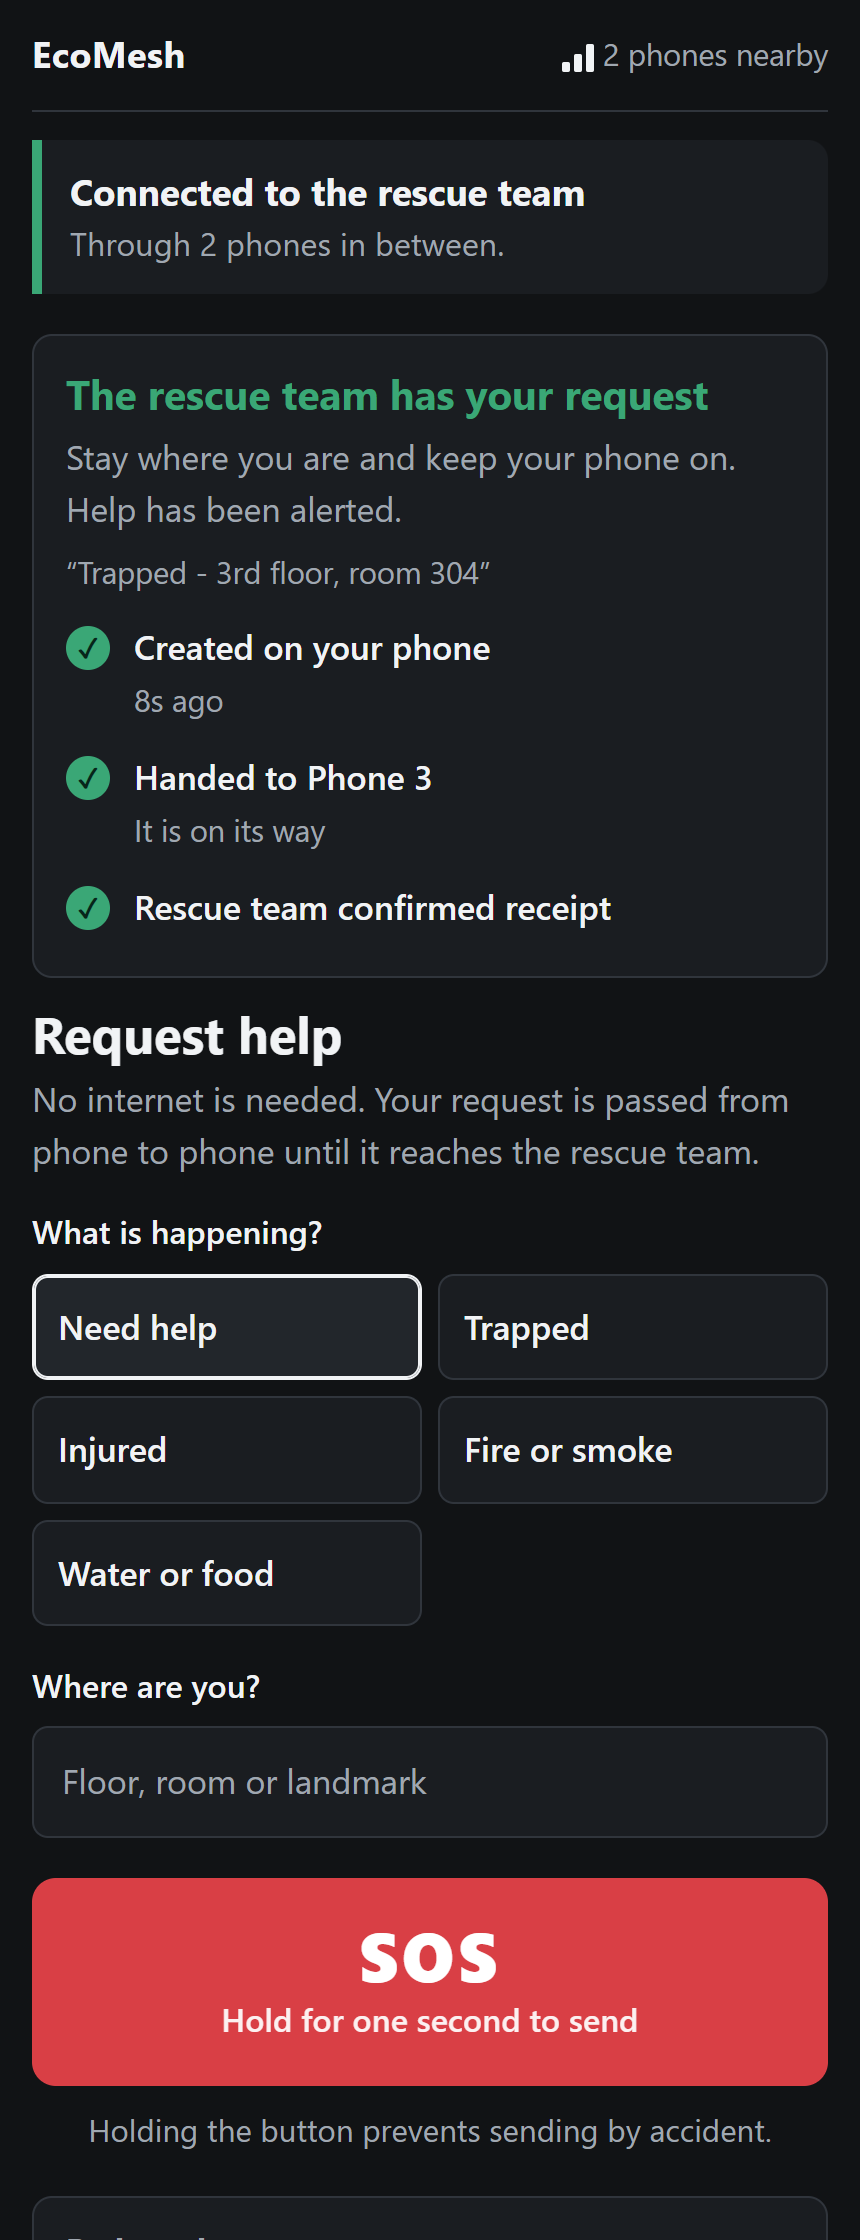
\includegraphics[width=\textwidth]{figures/story_survivor_delivered.png}\end{minipage}\hfill
\begin{minipage}[t]{0.22\textwidth}\centering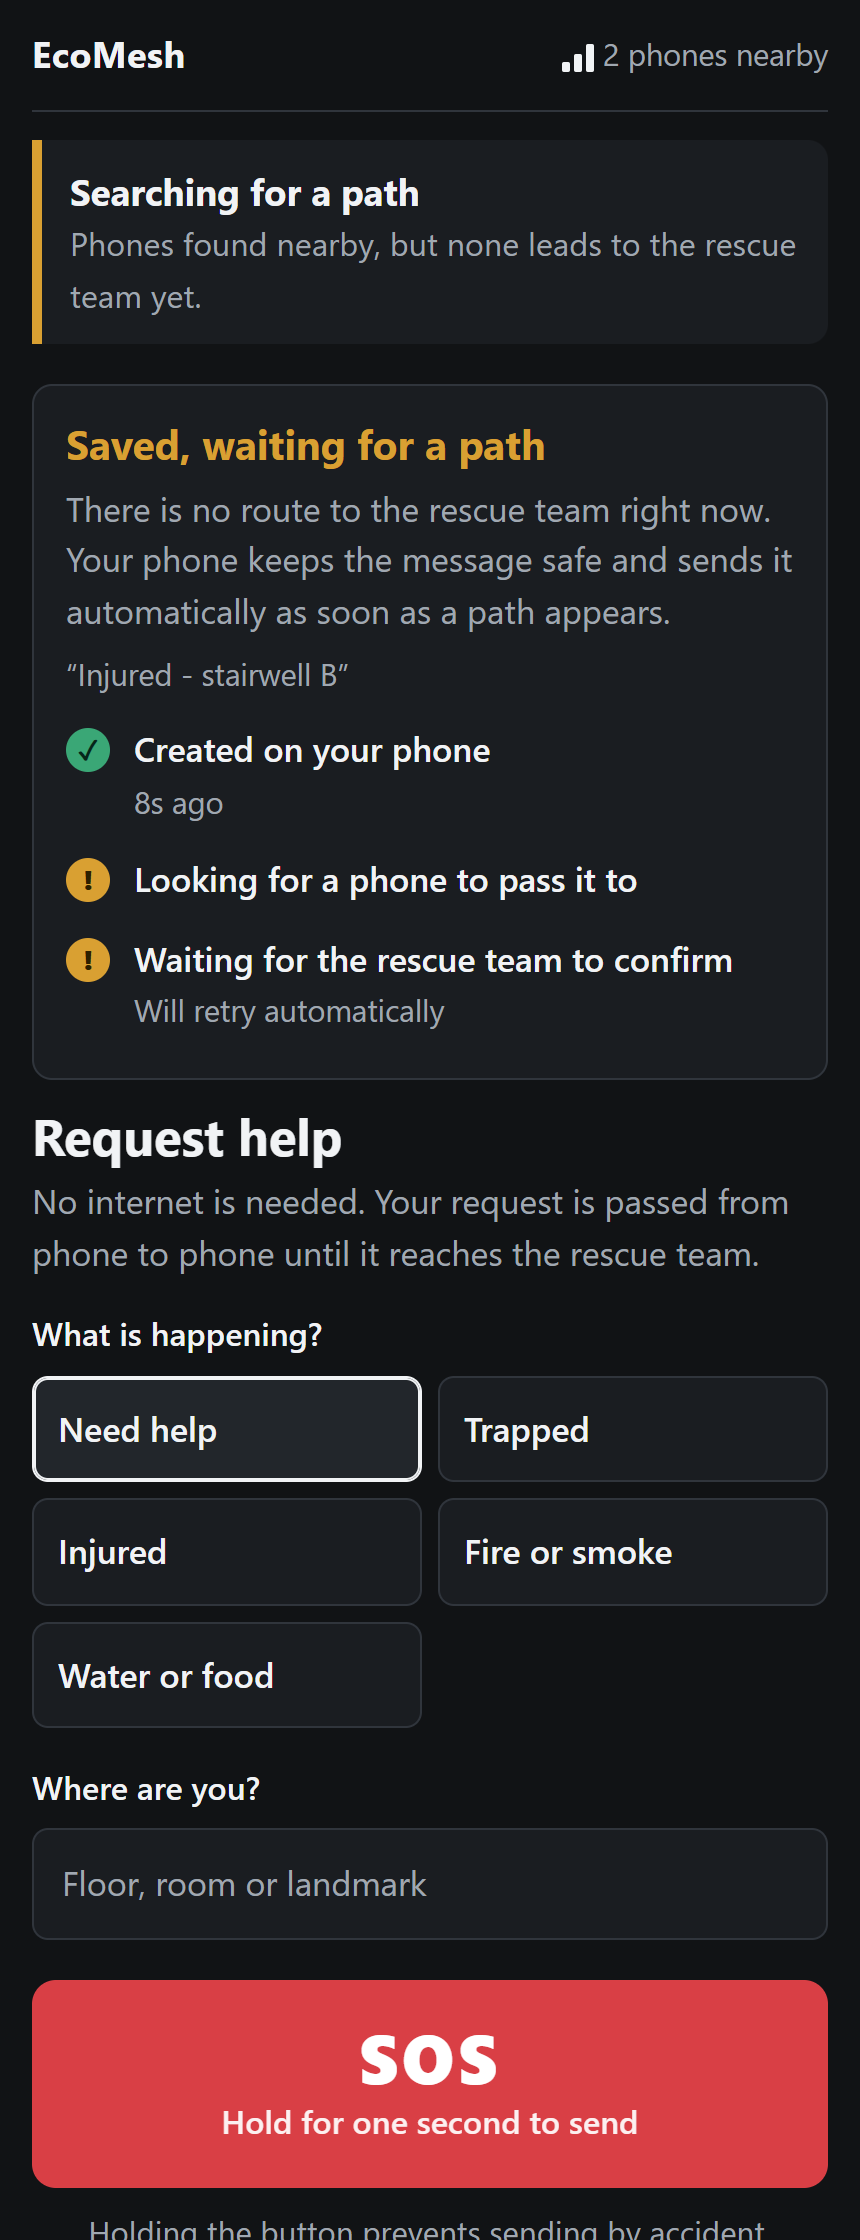
\includegraphics[width=\textwidth]{figures/story_survivor_held.png}\end{minipage}\hfill
\begin{minipage}[t]{0.22\textwidth}\centering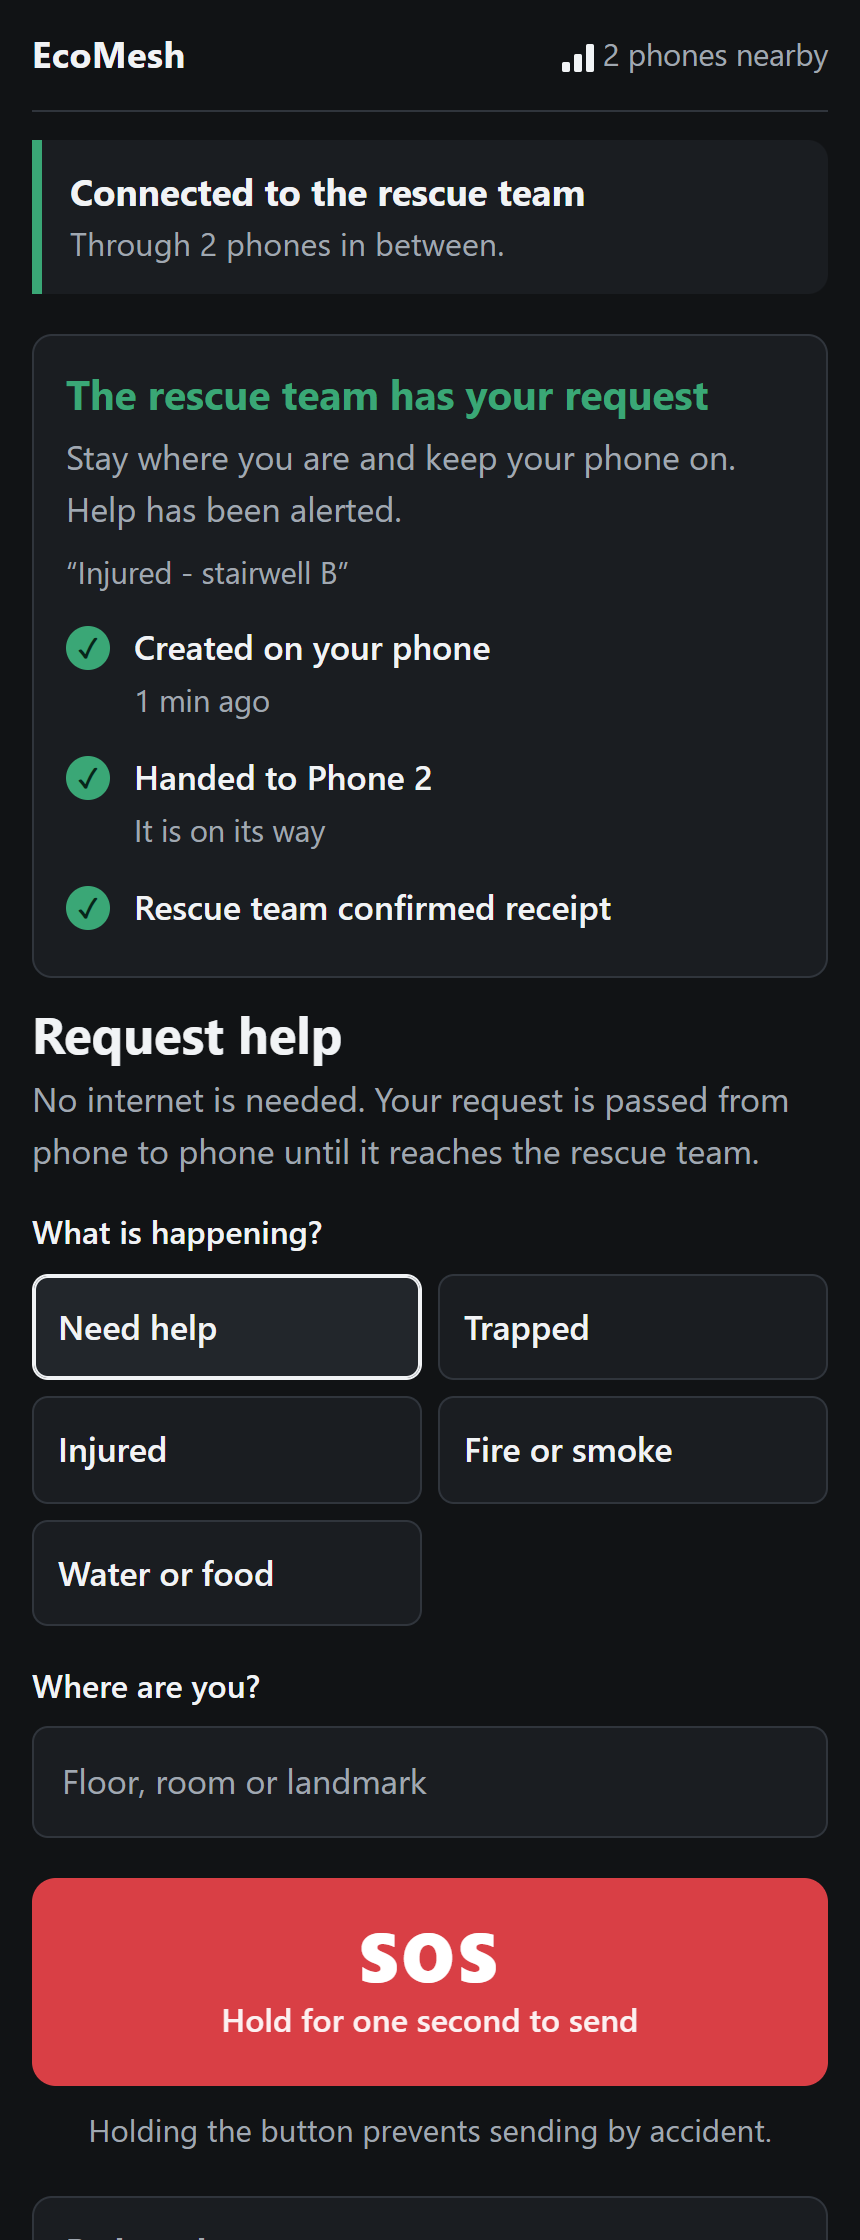
\includegraphics[width=\textwidth]{figures/story_survivor_flushed.png}\end{minipage}
\caption[The survivor's screen: delivered, held and flushed]{The survivor's screen. Left: SOS delivered over a relay phone and the Gateway. Centre: the gateway has failed; the screen says ``Searching for a path'' and the message is ``Saved, waiting for a path''. Right: the gateway is back and the held message is delivered.}
\label{fig:survivor}
\end{figure}
\begin{figure}[!htbp]
\centering
\begin{minipage}[t]{0.43\textwidth}\centering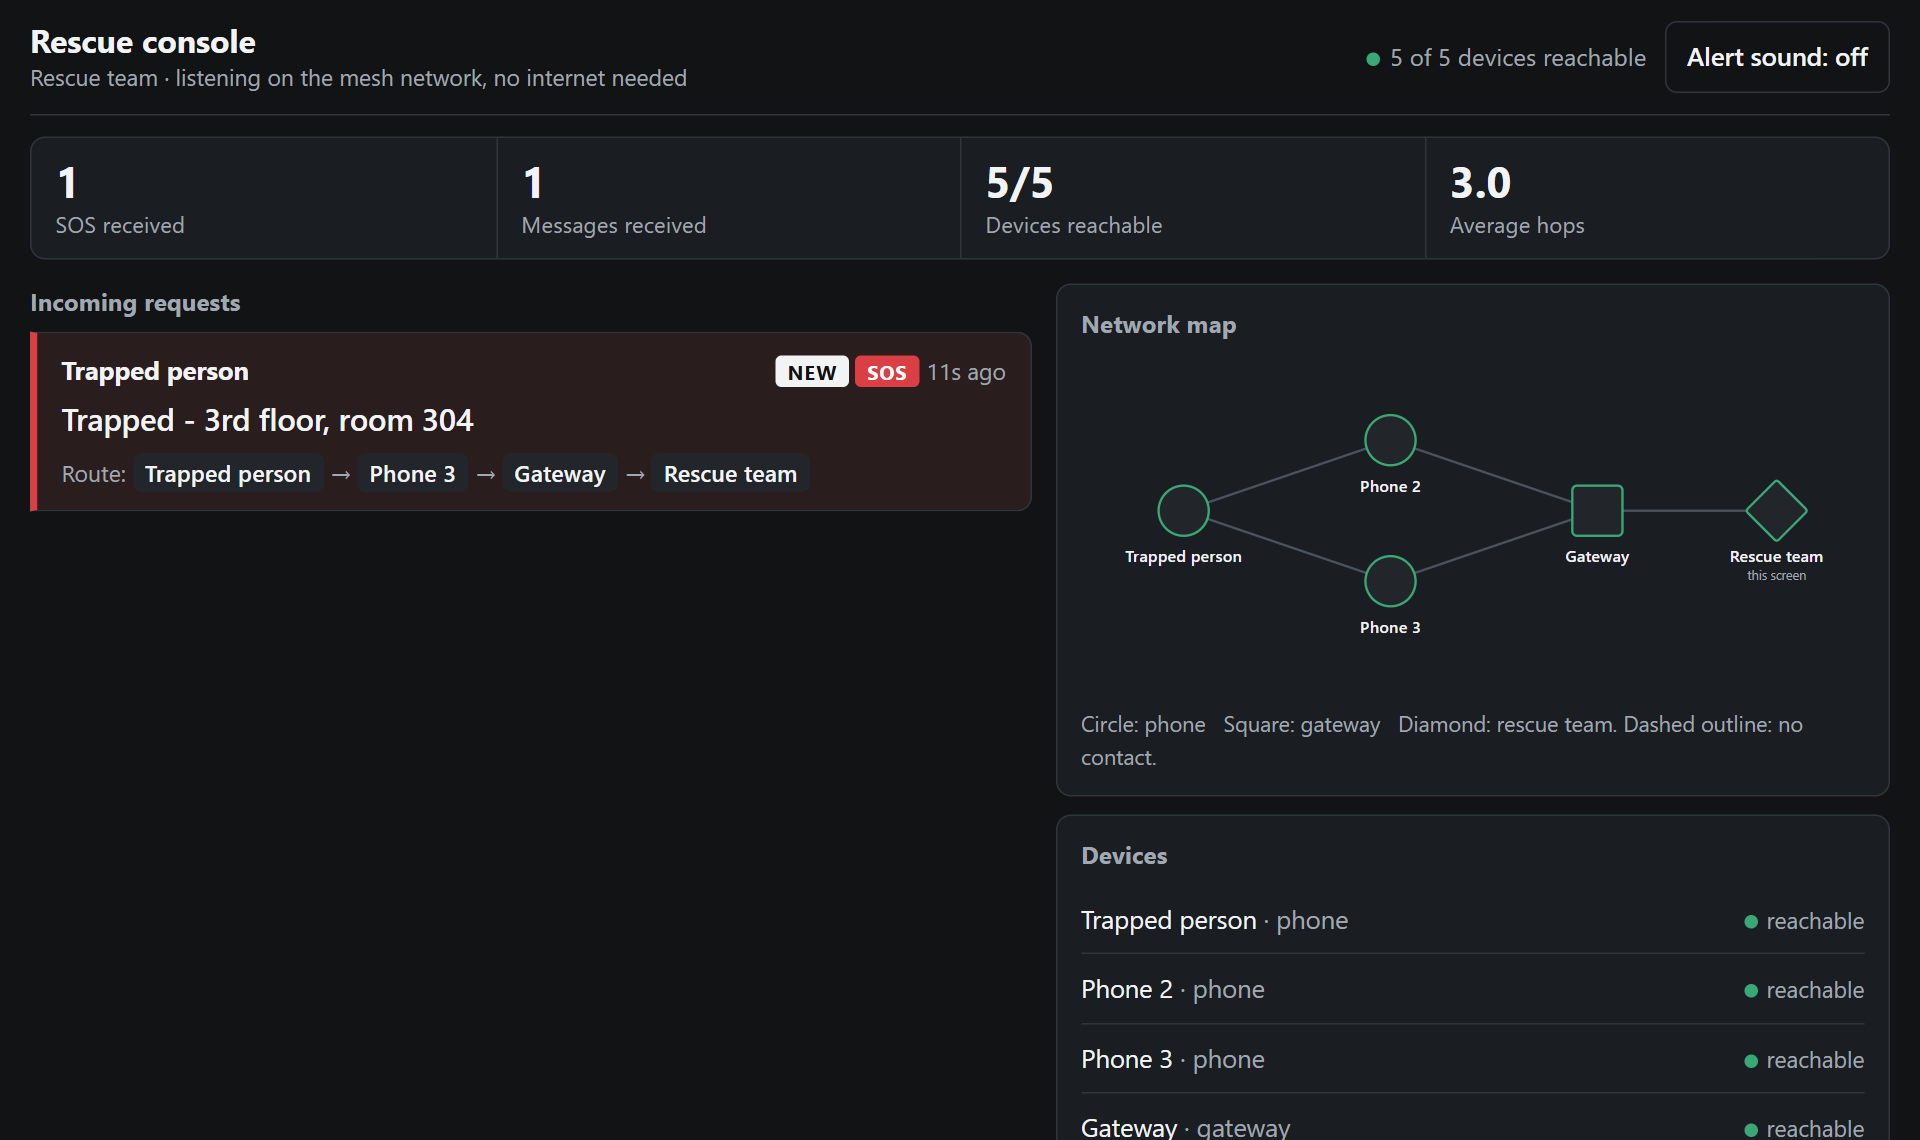
\includegraphics[width=\textwidth]{figures/story_rescue_console.png}\end{minipage}\hfill
\begin{minipage}[t]{0.43\textwidth}\centering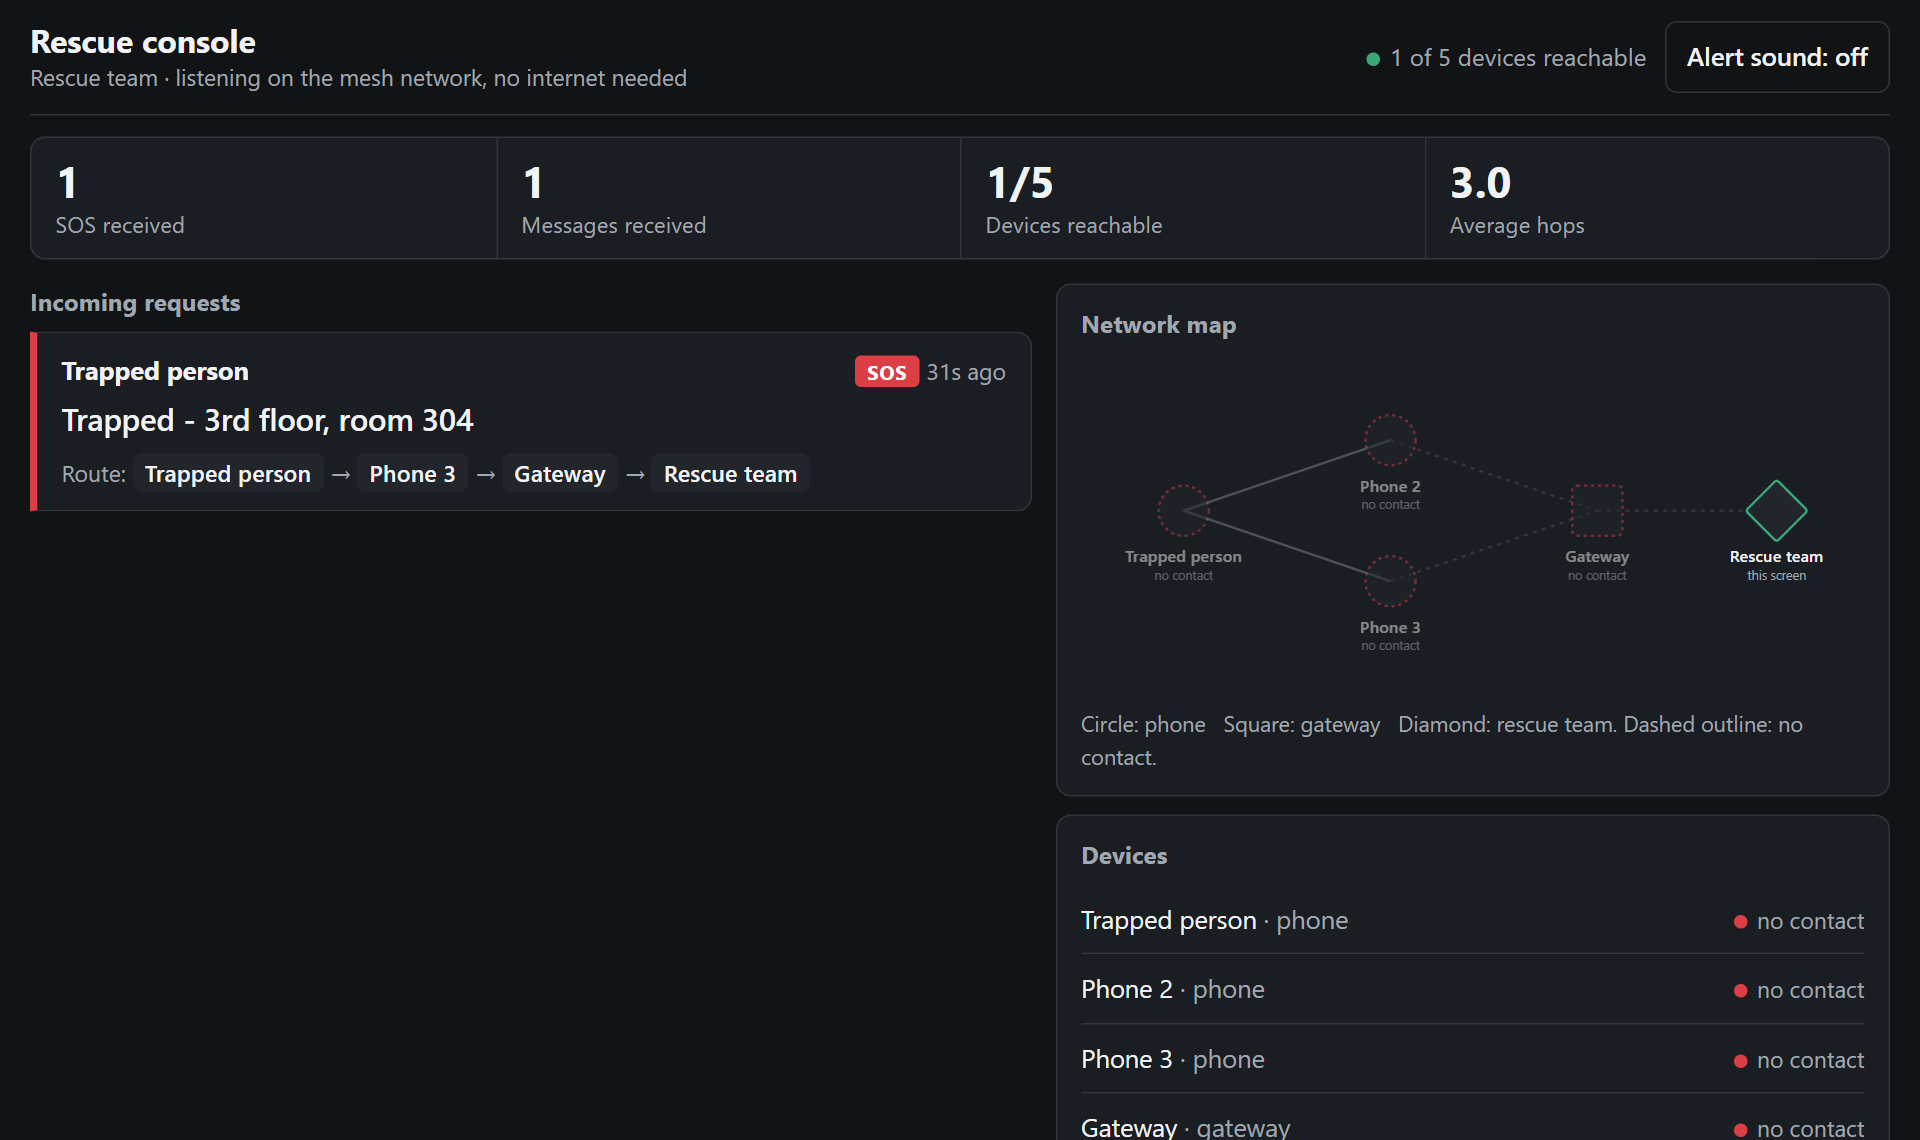
\includegraphics[width=\textwidth]{figures/story_rescue_console_gwdown.png}\end{minipage}
\caption[The rescue console, before and during a gateway outage]{The rescue console. Left: SOS cards with sender, text, age and route, counters, network map and device list. Right: with the gateway down the rescue device hears nobody (``1 of 5 devices reachable''); earlier messages remain visible.}
\label{fig:console}
\end{figure}
\begin{figure}[!htbp]
\centering
\begin{minipage}[t]{0.42\textwidth}\centering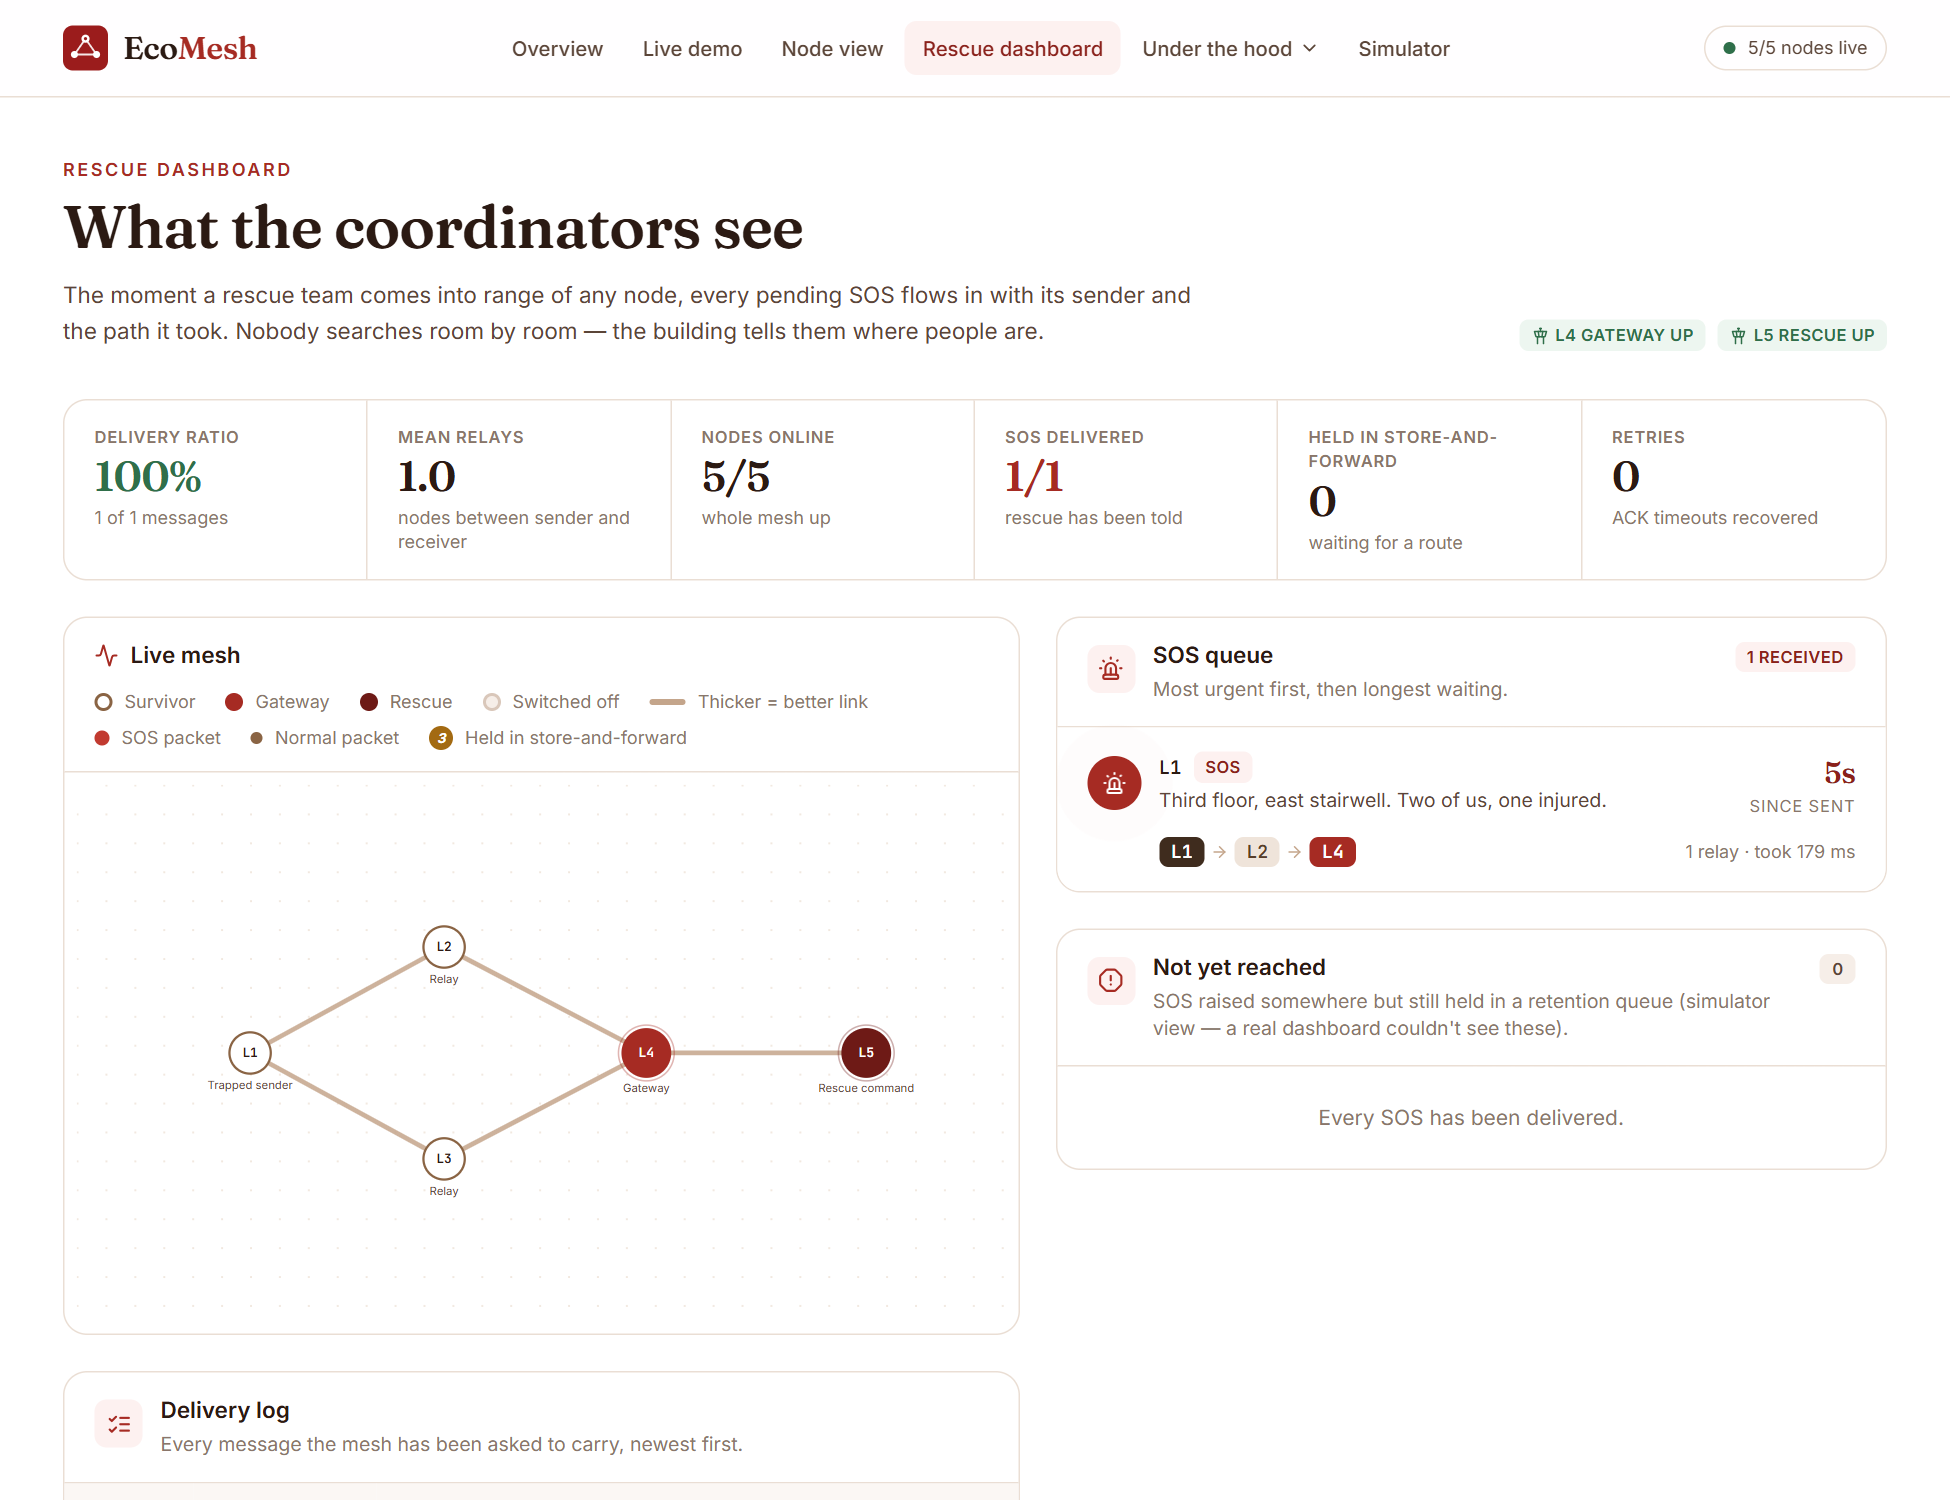
\includegraphics[width=\textwidth]{figures/ui_rescue.png}\end{minipage}\hfill
\begin{minipage}[t]{0.42\textwidth}\centering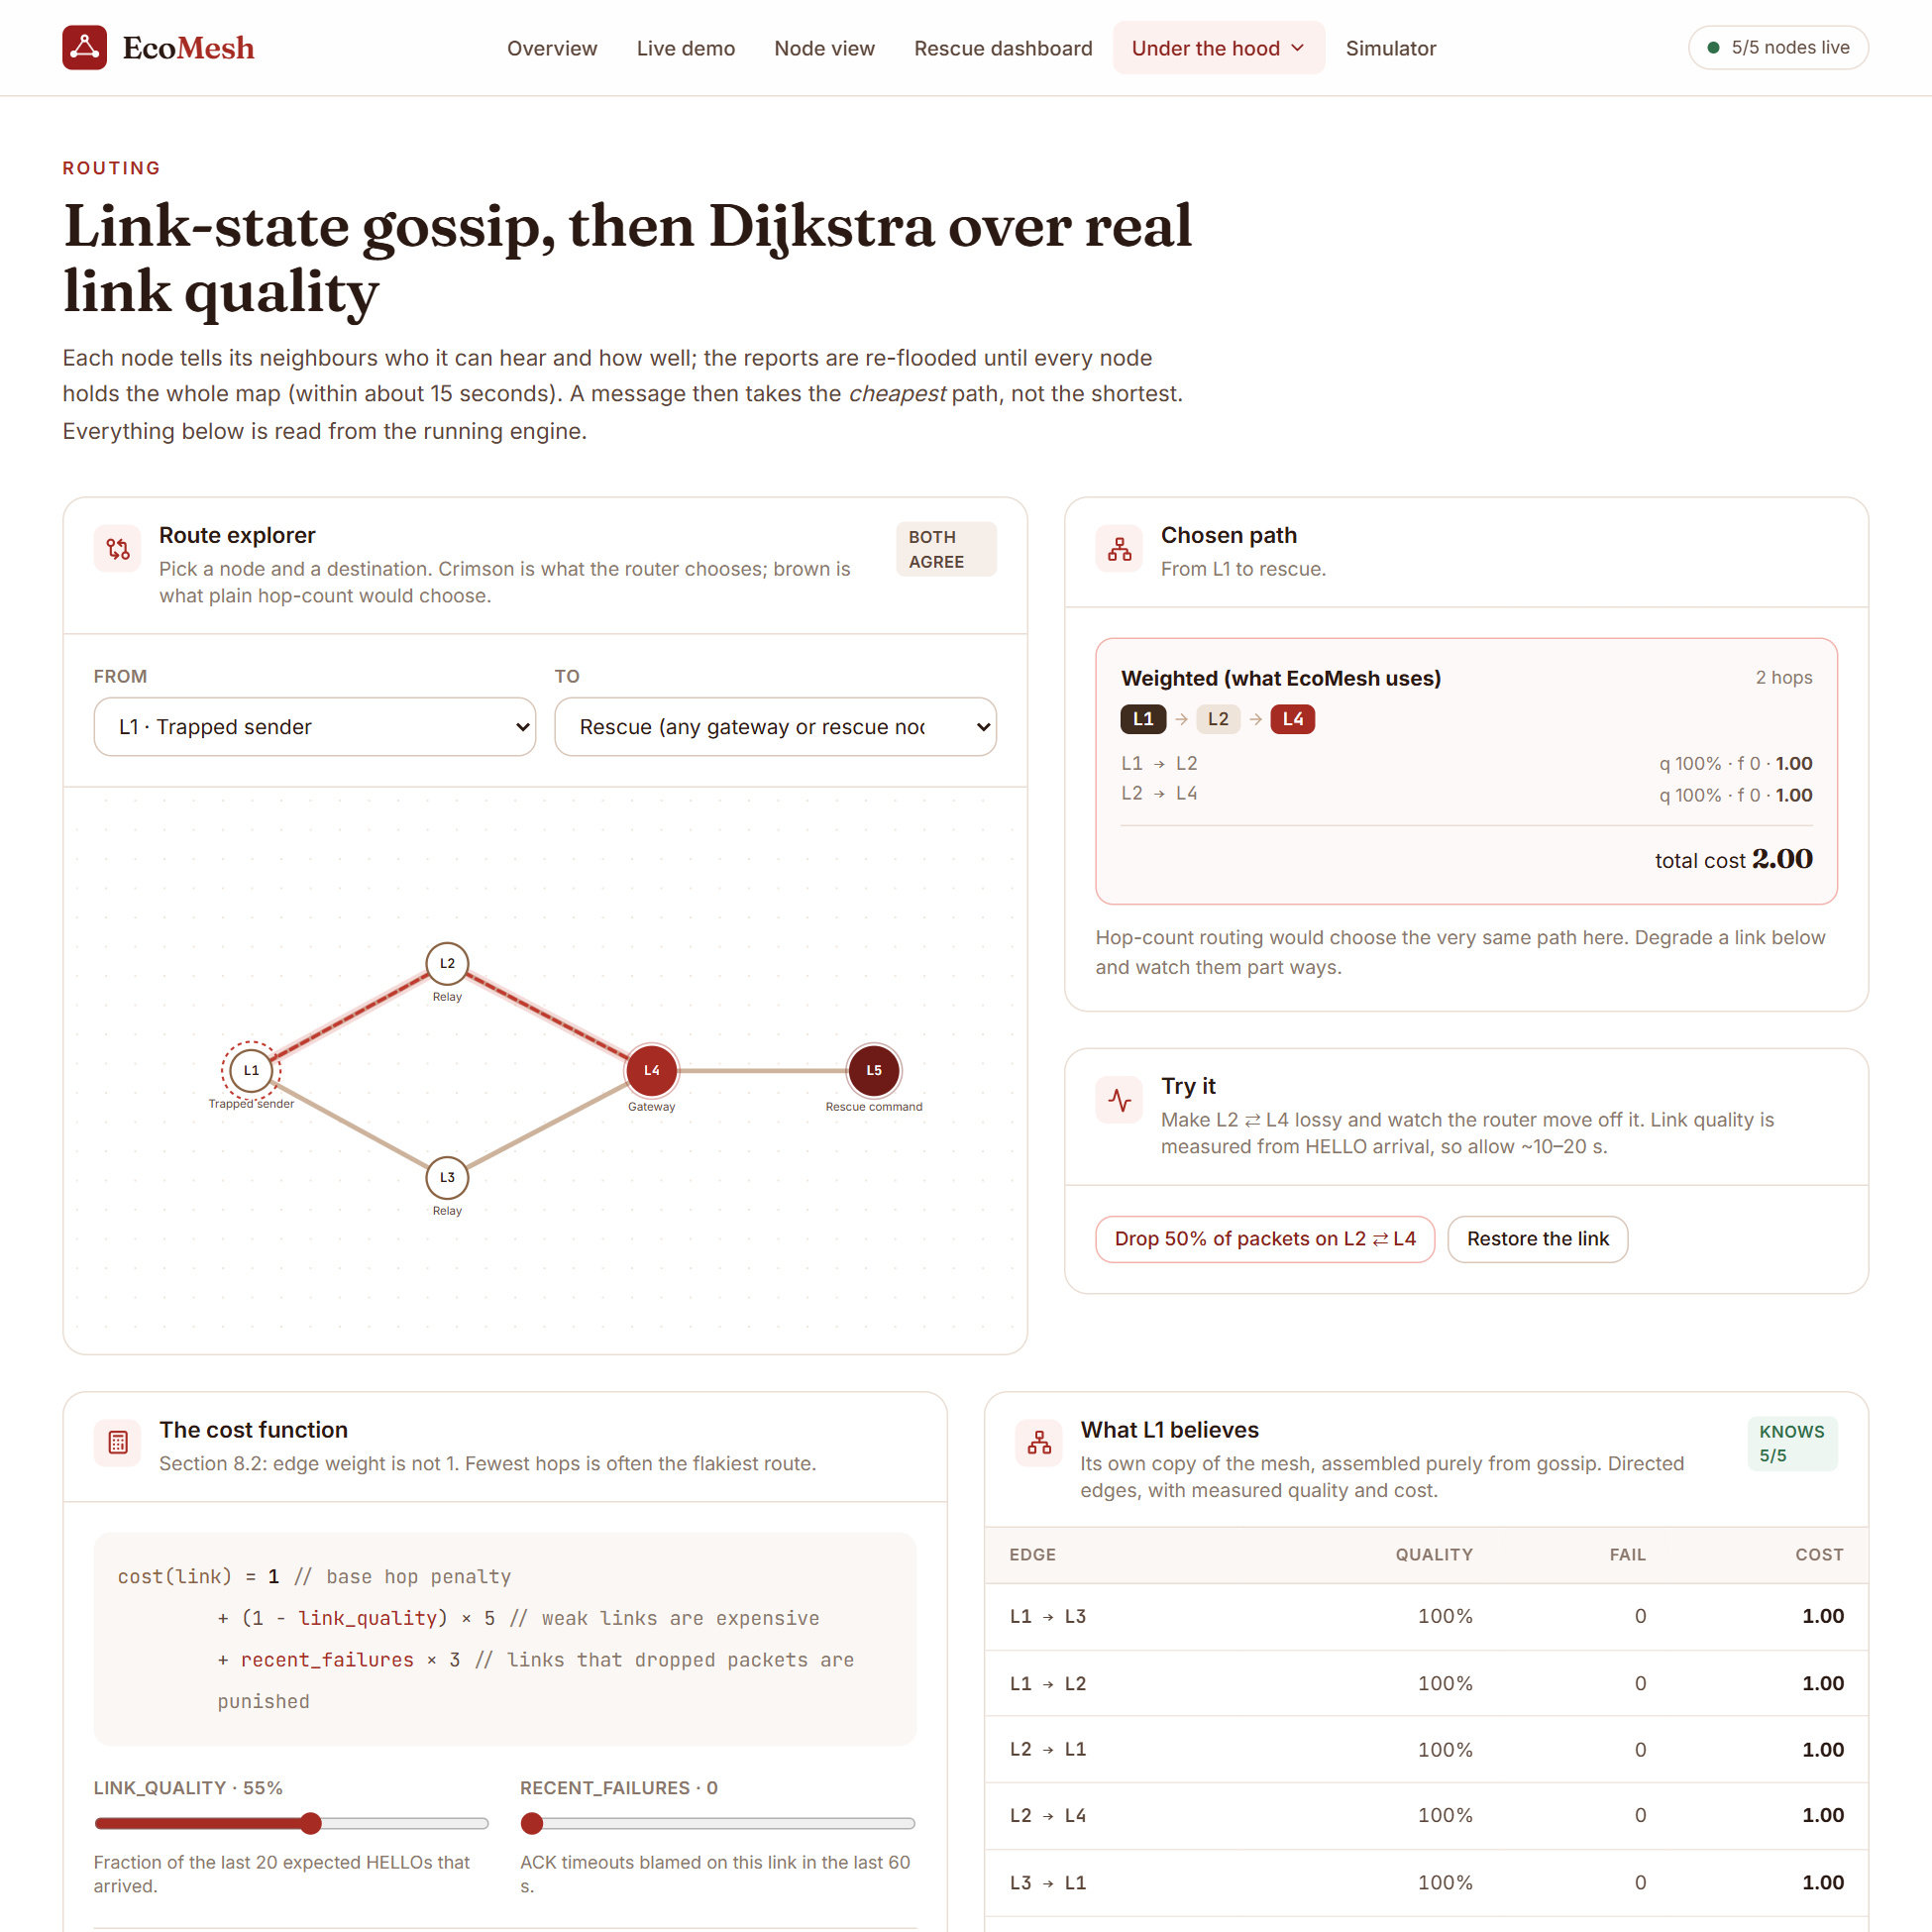
\includegraphics[width=\textwidth]{figures/ui_routing.png}\end{minipage}
\caption[The engine web application: rescue dashboard and routing page]{The engine web application. Left: rescue dashboard (delivery ratio, nodes online, live mesh, SOS queue). Right: routing page (weighted versus hop-count route, cost function, a node's view of the graph). A six-beat live demonstration page drives the same API.}
\label{fig:uishots}
\end{figure}
The mesh was also run on two physical laptops joined by a phone hotspot (Figure~\ref{fig:deploy}): an SOS was delivered across both machines, the route changed when a relay was switched off, and a message held while the gateway was off was delivered when it returned. This run was a functional demonstration and was not timed.

\subsection{Functional Results}
Of the 68 requirements, \NAuto\ are verified by automated tests alone, \NAutoUI\ with a manual screen check, \NInspect\ by inspection, \NManual\ manually, and \NPartial\ are partial (Table~\ref{tab:frsum}). The three key stories ran on real devices: an SOS reaches rescue over several hops, the mesh re-routes around a failed relay, and a message with no route is held and later delivered.
\subsection{Performance Results}
Table~\ref{tab:kpival} collects the measured KPIs: \CollDel\,\% delivery on 40 nodes at 20\,\% loss with failures, an SOS \SosAdv$\times$ faster under load, live SOS delivery in a median 47\,ms, relay failover in about 4\,s and held messages flushed in about 4.5\,s.
\subsection{Comparison with Existing Systems}
Other systems were not run, so the comparison uses documented properties (Table~\ref{tab:compare1}) and the one fair measurable baseline, hop-count routing on identical seeds (\HopW\,\% against \HopH\,\%). No claim is made about the delivery of Bridgefy, Briar, Meshtastic or Serval, which publish no comparable measurements.
\subsection{Achievement of Objectives}
Table~\ref{tab:objectives} maps each objective of Section~1.4 to its evidence and status.
\begin{table}[!htbp]
\caption{Objectives, supporting evidence and status}
\label{tab:objectives}
\footnotesize
\begin{tabularx}{\textwidth}{@{}>{\raggedright\arraybackslash}p{0.9cm}>{\raggedright\arraybackslash}X>{\raggedright\arraybackslash}p{3.4cm}@{}}
\toprule
\textbf{Obj.} & \textbf{Evidence} & \textbf{Status}\\ \midrule
O1 & live convergence 3.8\,s; simulator 5--15\,s in multiples of the gossip interval & Achieved (47 of 50 runs $\le$ 15\,s)\\
O2 & \HopW\,\% vs \HopH\,\% on \HopRuns\ identical seeds (Figure~\ref{fig:results}b) & Achieved\\
O3 & \SosAdv$\times$ lower median latency under load (Section~\ref{sec:perfresults}) & Achieved\\
O4 & \CollDel\,\% at 40 nodes and 20\,\% loss; recovery mean \CollRecMean\,s, \CollRecOK\ of \CollRecN\ trials within 10\,s & Partly achieved\\
O5 & 201 of 201 flushed in simulation; 4 of 4 live outages & Achieved\\
O6 & security tests (Section~\ref{sec:nonfunc}) & Achieved with a pre-shared key\\
O7 & every metric is a query over per-node logs & Achieved\\
O8 & web application, device screens, API tests, five processes, two laptops & Achieved\\
\bottomrule
\end{tabularx}
\end{table}

\subsection{Discussion of Findings}
Hop count is a poor proxy for delivery: a weak shortcut loses almost half the traffic under hop count and almost none under the weighted cost. Timer constants, not algorithms, set recovery and convergence (they cluster at the heartbeat timeout and the gossip interval), which shows exactly what to tune. Loss is paid for in tail latency, and priority matters only once a link queues, which is the disaster condition. Testing found real defects in code we believed finished (Section~\ref{sec:defects}).

\subsection{Practical Applicability}
A deployment needs devices running the node program, a topology file (or multicast discovery), a gateway or rescue device and a shared network segment. It is usable today as a campus, hospital or building safety system on laptops; a Bluetooth LE or Wi-Fi Direct transport would make it phone-to-phone.

\section{Conclusion and Future Scope}
\label{ch:concl}
\providecommand{\HopW}{99.2}\providecommand{\HopH}{57.4}\providecommand{\HopWins}{20}\providecommand{\HopRuns}{20}

\providecommand{\SosAdv}{4.4}

\providecommand{\CollN}{50}\providecommand{\CollDel}{92.6}\providecommand{\CollDelMin}{76}\providecommand{\CollDelMax}{100}\providecommand{\CollRecMean}{8.1}\providecommand{\CollRecMax}{10.25}\providecommand{\CollRecN}{50}\providecommand{\CollRecOK}{23}\providecommand{\CollConvMean}{9.6}\providecommand{\CollConvMax}{15.2}


\subsection{Conclusion}
Every mainstream messaging tool fails when its infrastructure fails, although devices in a stricken building can still reach each other. We built EcoMesh, a peer-to-peer mesh in which every device is an endpoint and a relay, with a complete engine, a simulator that measures it, a REST/WebSocket interface, two front ends and a multi-device deployment over TCP. Weighted routing delivered \HopW\,\% of messages where hop-count routing delivered \HopH\,\% on identical seeds; an SOS had a \SosAdv$\times$ lower median latency under load; a 40-node mesh at 20\,\% loss with injected failures delivered \CollDel\,\% over 50 runs; and on five live processes an SOS arrived in a median of 32\,ms, the sender re-routed around a failed relay in about 4.1\,s, and every message held during a gateway outage was delivered when the gateway returned.

\subsection{Achievement of Objectives}
Objectives O1--O3 and O5--O8 were achieved. O4 was achieved for delivery but only partly for recovery time, where 26 of 50 trials exceeded 10\,s by at most 0.25\,s, the heartbeat timeout (Table~\ref{tab:objectives}).

\subsection{Major Engineering Contributions}
A transport-agnostic engine that runs unchanged on a simulator and on real sockets; a derived link-quality cost function with an immediate failure penalty and network-wide re-flooding; per-hop priority with a bounded queue that never evicts an SOS for routine traffic; signatures that survive multi-hop relaying; and a measurement framework in which every number in this report is generated from per-node logs and stored results.


\subsection{Current Limitations}
As detailed in Section~\ref{sec:limits}: a neighbour-restricted LAN stands in for a radio; one pre-shared key serves the mesh; relays do not retain; timer constants quantise recovery and convergence; there is no usability study with participants, and the browser checks are scripts run by hand rather than part of the automated suite; there is no phone application, only a web page that a phone opens over the same Wi-Fi; and scale was tested to 65 simulated nodes.


\subsection{Future Enhancements}
(1) A Bluetooth LE or Wi-Fi Direct transport and an Android client speaking the same protocol. (2) Adaptive timers: a shorter fixed neighbour timeout (about 7\,s) was tried and dropped because it lowered delivery at 20\,\% loss, so the next step is a timeout adapted to each link, an immediate report on topology change and an ACK timeout derived from the measured round-trip time. (3) X25519 per-pair key agreement. (4) Short retention at relays, so that a relay does not lose a message it has accepted. (5) Per-destination route invalidation. (6) A usability study, running the browser checks inside the automated suite, a stable ordering for messages created in the same millisecond (D7), and tests beyond 65 nodes.

\subsection{Lessons Learned}
Build the simulator first and draw the transport boundary before the layers: it paid for itself in testing and in deployment. Integration finds what unit tests do not (the multi-hop ACK bug survived every single-node test). Look at distributions as well as means: recovery clustered at the heartbeat timeout, which the mean hid. Record who built what from the first week, with consistent Git identities.



% thebibliography starts its own page (main.tex: every \section begins one),
% so the contents entry is added inside it, on the References page itself.
\footnotesize
\begin{thebibliography}{99}
\phantomsection\addcontentsline{toc}{section}{References}
\setlength{\itemsep}{0.5pt}
\bibitem{albrecht2021bridgefy}
M.~R. Albrecht, J.~Blasco, R.~B. Jensen and L.~Mare\v{k}ov\'a, ``Mesh Messaging in Large-scale Protests: Breaking Bridgefy,'' in \emph{Topics in Cryptology -- CT-RSA 2021}, Lecture Notes in Computer Science, vol.~12704, Springer, 2021, pp.~375--398.

\bibitem{perkins1994dsdv}
C.~E. Perkins and P.~Bhagwat, ``Highly dynamic Destination-Sequenced Distance-Vector routing (DSDV) for mobile computers,'' in \emph{Proc. ACM SIGCOMM}, 1994, pp.~234--244.

\bibitem{rfc4728dsr}
D.~Johnson, Y.~Hu and D.~Maltz, ``The Dynamic Source Routing Protocol (DSR) for Mobile Ad Hoc Networks for IPv4,'' RFC~4728, IETF, Feb. 2007.

\bibitem{rfc3561aodv}
C.~Perkins, E.~Belding-Royer and S.~Das, ``Ad hoc On-Demand Distance Vector (AODV) Routing,'' RFC~3561, IETF, July 2003.

\bibitem{rfc3626olsr}
T.~Clausen and P.~Jacquet (eds.), ``Optimized Link State Routing Protocol (OLSR),'' RFC~3626, IETF, Oct. 2003.

\bibitem{rfc2328ospf}
J.~Moy, ``OSPF Version 2,'' RFC~2328, IETF, Apr. 1998.

\bibitem{rfc8966babel}
J.~Chroboczek and D.~Schinazi, ``The Babel Routing Protocol,'' RFC~8966, IETF, Jan. 2021.

\bibitem{decouto2003etx}
D.~S.~J. De Couto, D.~Aguayo, J.~Bicket and R.~Morris, ``A high-throughput path metric for multi-hop wireless routing,'' in \emph{Proc. ACM MobiCom}, 2003, pp.~134--146.

\bibitem{vahdat2000epidemic}
A.~Vahdat and D.~Becker, ``Epidemic Routing for Partially-Connected Ad Hoc Networks,'' Technical Report CS-2000-06, Duke University, 2000.

\bibitem{fall2003dtn}
K.~Fall, ``A delay-tolerant network architecture for challenged internets,'' in \emph{Proc. ACM SIGCOMM}, 2003, pp.~27--34.

\bibitem{rfc4838}
V.~Cerf \emph{et al.}, ``Delay-Tolerant Networking Architecture,'' RFC~4838, IETF, Apr. 2007.

\bibitem{reina2015disaster}
D.~G. Reina, M.~Askalani, S.~L. Toral, F.~Barrero, E.~Asimakopoulou and N.~Bessis, ``A survey on multihop ad hoc networks for disaster response scenarios,'' \emph{International Journal of Distributed Sensor Networks}, vol.~11, no.~10, art.~647037, 2015.

\bibitem{nist80038d}
M.~Dworkin, ``Recommendation for Block Cipher Modes of Operation: Galois/Counter Mode (GCM) and GMAC,'' NIST Special Publication 800-38D, Nov. 2007.

\bibitem{bernstein2012ed25519}
D.~J. Bernstein, N.~Duif, T.~Lange, P.~Schwabe and B.-Y. Yang, ``High-speed high-security signatures,'' \emph{Journal of Cryptographic Engineering}, vol.~2, no.~2, pp.~77--89, 2012.

\bibitem{dijkstra1959}
E.~W. Dijkstra, ``A note on two problems in connexion with graphs,'' \emph{Numerische Mathematik}, vol.~1, pp.~269--271, 1959.

\bibitem{briar}
The Briar Project, ``Briar: secure messaging anywhere -- how it works,'' \url{https://briarproject.org}, accessed 2026.

\bibitem{meshtastic}
Meshtastic, ``Mesh Broadcast Algorithm'' and ``Why Meshtastic uses managed flood routing,'' documentation, \url{https://meshtastic.org/docs/overview/mesh-algo/}, accessed 2026.

\bibitem{serval}
The Serval Project, ``Serval: communications for disaster and remote areas'' (including the Rhizome data-distribution protocol), project documentation, \url{https://www.servalproject.org}, accessed 2026.
\end{thebibliography}

% The department Mini Project template ends with "Research Paper/ Poster" and
% "Plagiarism Report" after the conclusion; both are inserted at this page.
\section*{Appendix: Research Paper / Poster and Plagiarism Report}
\addcontentsline{toc}{section}{Appendix: Research Paper / Poster and Plagiarism Report}
\label{app:paper}\label{app:plag}
\noindent As the department template requires, the end-semester research paper or poster (with, if accepted for
publication, the acceptance receipt or certificate) and the plagiarism report of this report, generated with the
college-approved checker, are inserted after this page.

\vspace{8mm}
\noindent\fbox{\parbox{\dimexpr\textwidth-2\fboxsep-2\fboxrule}{\centering\vspace{6mm}
\textbf{[Insert the research paper or poster here]}\par\vspace{6mm}}}

\vspace{6mm}
\noindent\fbox{\parbox{\dimexpr\textwidth-2\fboxsep-2\fboxrule}{\centering\vspace{6mm}
\textbf{[Insert the plagiarism report here]}\par\vspace{6mm}}}


\end{document}
